\documentclass{muthesis2021}
\usepackage[authoryear,round]{natbib}
\setcounter{secnumdepth}{4}
\usepackage{graphicx}
\usepackage{latexsym}
\usepackage{amsmath}
\usepackage{amsthm}
\usepackage{url}
\urlstyle{same}
\usepackage{textcomp}

\usepackage{caption,setspace}
\captionsetup{font={stretch=1.5}}

\usepackage{tikz}
\usetikzlibrary{shapes.geometric, arrows.meta, positioning, calc}
\usepackage{pgfplots}
\pgfplotsset{compat=1.18}

\usepackage{booktabs}
\usepackage{multirow}
\usepackage{amssymb}

\usepackage{microtype}
\usepackage{hyphenat}
\emergencystretch=1em

\usepackage[flushleft]{threeparttable}
\newcommand\mathplus{+}

\makeatletter
\renewcommand{\@dotsep}{10000}
\setlength{\@fptop}{0pt}
\setlength{\@fpbot}{0pt plus 1fil}
\makeatother

\title{Explainable Feature Drift Detection for MLOps Monitoring}
\author{Nusrat Begum}

\input{preamble}

\begin{document}

\maketitle

\linespacing{1.5}
\input{acknowledgements}
\abstract{
Machine learning models in production suffer silent performance degradation from distribution drift. Existing unsupervised detectors signal \textit{that} drift occurred but not \textit{which} features drifted or \textit{what} corrective action to take. This thesis proposes Explainable Adversarial Drift Detection (EADD), integrating discriminative classification with an entropy-based Prediction Uncertainty Index for early warning, adaptive sequential permutation testing, SHAP interaction-aware drift localization, and a novel Drift Severity Index for automated remediation prescriptions. Evaluated against seven state-of-the-art detectors across synthetic and real-world benchmarks, EADD uniquely achieved complete drift-type coverage with near-zero false alarms while providing feature-level root-cause attribution ($P@k=R@k=1.0$). The adaptive permutation test reduced computational overhead by up to 70\% compared to fixed-budget approaches while maintaining statistical rigor.
}{
% ภาษาไทย (Thai Abstract Placeholder)
% โปรดใส่บทคัดย่อภาษาไทยที่นี่
}


\tableofcontents
\listoftables
\listoffigures

%\chapter{Introduction} \label{chap:intro}

\section{Motivation}
Machine learning models deployed in real-world environments frequently encounter evolving data distributions over time. According to \citet{Lu2018} and \citet{Gama2014}, these changes---collectively referred to as distribution shift or drift---can manifest as changes in input features (covariate drift) or in the relationship between inputs and labels (concept drift), causing model performance to deteriorate if left unmanaged. \citet{Lu2018} and \citet{WidmerKubat1996} emphasize that detecting such changes early is essential for maintaining reliable model performance, reducing operational risk, and avoiding the accumulation of technical debt in production systems \citep{Bayram2022, Sculley2015}.

Conventional model monitoring strategies react to drift only after observable performance degradation, which by design means that the system has already suffered from poor predictions on new data \citep{WidmerKubat1996}. In production contexts where ground-truth labels may be delayed, unavailable, or costly to obtain, this post-hoc reactive approach is often inadequate \citep{Lu2018, Souza2020}. According to \citet{Lu2018} and \citet{Bayram2022}, early drift detection that anticipates distribution changes before significant performance loss is therefore a practical priority in dynamic machine learning systems.

The consequences of undetected covariate drift are severe. \citet{Vela2022} demonstrated empirically that AI model performance degrades significantly over time as a direct consequence of temporal distribution shift, with clinical prediction models showing measurable accuracy losses within months of deployment. \citet{NestorEtAl2019} reinforced this finding by showing that machine learning models for common clinical tasks failed to maintain performance when applied to temporally shifted patient cohorts, even within the same hospital system. In these high-stakes environments, a simple ``drift detected'' alarm is insufficient; practitioners and engineers require immediate root-cause explanations to determine whether the degradation stems from specific feature pipelines, population-level shifts, or systemic data quality issues \citep{Sculley2015}.

Current drift detection methods vary considerably in their assumptions and approach. Traditional statistical methods employ hypothesis tests---such as the Kolmogorov--Smirnov test, chi-squared test, or Kullback--Leibler divergence---to detect distribution changes by comparing incoming and reference data \citep{Rabanser2019, Raab2020}. \citet{BifetGavalda2007} developed adaptive windowing methods like ADWIN that dynamically adjust how much historical data is retained for comparison. Supervised error-based detectors like DDM and EDDM monitor model performance metrics over time, but require access to ground-truth labels \citep{Gama2004, BaenaGarcia2006}. Prediction-based detectors track model outputs for changes in confidence, entropy, or prediction distributions without necessarily requiring labels \citep{Sethi2017}. Despite this diversity, several challenges remain: statistical tests can be sensitive to noise and may struggle in high-dimensional settings; supervised methods depend on label availability; prediction-based methods may be confounded by model calibration issues; and hybrid approaches often require engineered context variables that may not generalize across domains \citep{Lu2018, Webb2016}.

To address these gaps, we build on the insight of recasting distribution comparison as a discriminative learning problem. \citet{LopezPazOquab2017} formalized this as the \textit{classifier two-sample test} (C2ST): if an auxiliary classifier can reliably separate data from two sources based solely on features, the distributions differ significantly. This principle has been applied in data science for dataset shift detection \citep{Pan2020, Qian2021} and was adapted for streaming drift detection by \citet{Gozuacik2019} as the Discriminative Drift Detector (D3). However, existing implementations provide only a binary drift signal without explaining \textit{which} features drifted or \textit{what corrective action} is appropriate---a critical limitation for production MLOps systems.

According to \citet{LopezPazOquab2017}, the discriminative approach offers several key advantages: it is label-independent, model-agnostic, makes no assumptions about which features are important, and can detect complex high-dimensional, non-linear distributional shifts that evade univariate statistical tests. What remains missing is the integration of this detection capability with \textit{explainability}---the ability to attribute drift to specific features and map those attributions to actionable remediation strategies.

\section{Objectives}
The primary objective of this thesis is to develop \textbf{Explainable Adversarial Drift Detection (EADD)}, a framework that integrates adversarial validation, permutation-based significance testing, and SHAP-based feature attribution into a unified streaming drift detection pipeline. Specifically, this work aims to:

\begin{enumerate}
    \item Extend the discriminative drift detection approach of D3 \cite{Gozuacik2019} with a non-linear adversarial classifier (LightGBM) and \textbf{reservoir sampling} for representative reference windows, broadening detection coverage to gradual and incremental drift patterns where linear classifiers fail.
    
    \item Adapt the classifier two-sample test framework of \citet{LopezPazOquab2017} to streaming drift detection by integrating \textbf{permutation testing} for statistically principled threshold calibration, replacing the arbitrary fixed thresholds used in existing discriminative detectors.
    
    \item Develop a \textbf{SHAP-based root cause analysis} module that extracts feature-level drift attribution from the adversarial classifier, transforming the binary detection signal into a diagnostic report identifying \textit{which} features drive detected drift \citep{Lundberg2017}.
    
    \item Design an \textbf{automated prescription system} that maps SHAP importance patterns to actionable MLOps remediation strategies (univariate fix, partial retrain, or full retrain).
    
    \item Systematically benchmark EADD against state-of-the-art unsupervised drift detectors on the real-world datasets from the \citet{Lukats2025} benchmark, evaluating both detection accuracy and the practical value of explainability.
\end{enumerate}

\section{Expected Contributions}
This thesis contributes:

\begin{enumerate}
    \item \textbf{EADD Framework:} An integrated streaming drift detection pipeline that unifies adversarial validation (extending D3 \citep{Gozuacik2019}), permutation-based significance testing (adapting \citet{LopezPazOquab2017} for streaming contexts), and SHAP-based root cause analysis \citep{Lundberg2017} into a single coherent system. While individual components exist in isolation, no prior work has combined them into an end-to-end framework that provides statistically rigorous drift confirmation \textit{with} feature-level attribution.
    
    \item \textbf{Root Cause Analysis for Drift Detection:} Application of TreeSHAP feature attribution to the adversarial classifier to identify which specific features drive detected drift. This addresses the ``black box'' limitation of existing discriminative detectors \citep{Gozuacik2019, Lukats2025} and bridges the gap between detection and remediation.
    
    \item \textbf{Automated Prescriptions:} A systematic classification of drift patterns (univariate, feature-subset, multivariate) based on SHAP importance distributions, with corresponding actionable remediation recommendations for MLOps teams.
    
    \item \textbf{Benchmark Evaluation:} Comprehensive comparison with seven state-of-the-art unsupervised detectors on 13 real-world data streams from the \citet{Lukats2025} benchmark, demonstrating that explainability can be achieved without sacrificing detection accuracy.
    
    \item \textbf{Practical Guidelines:} Deployment recommendations for production MLOps pipelines, including window sizing, monitoring frequency, and computational efficiency trade-offs.
\end{enumerate}


\chapter{Literature Review} \label{chap:literature}

\begin{figure}[!htpb]
    \centering
    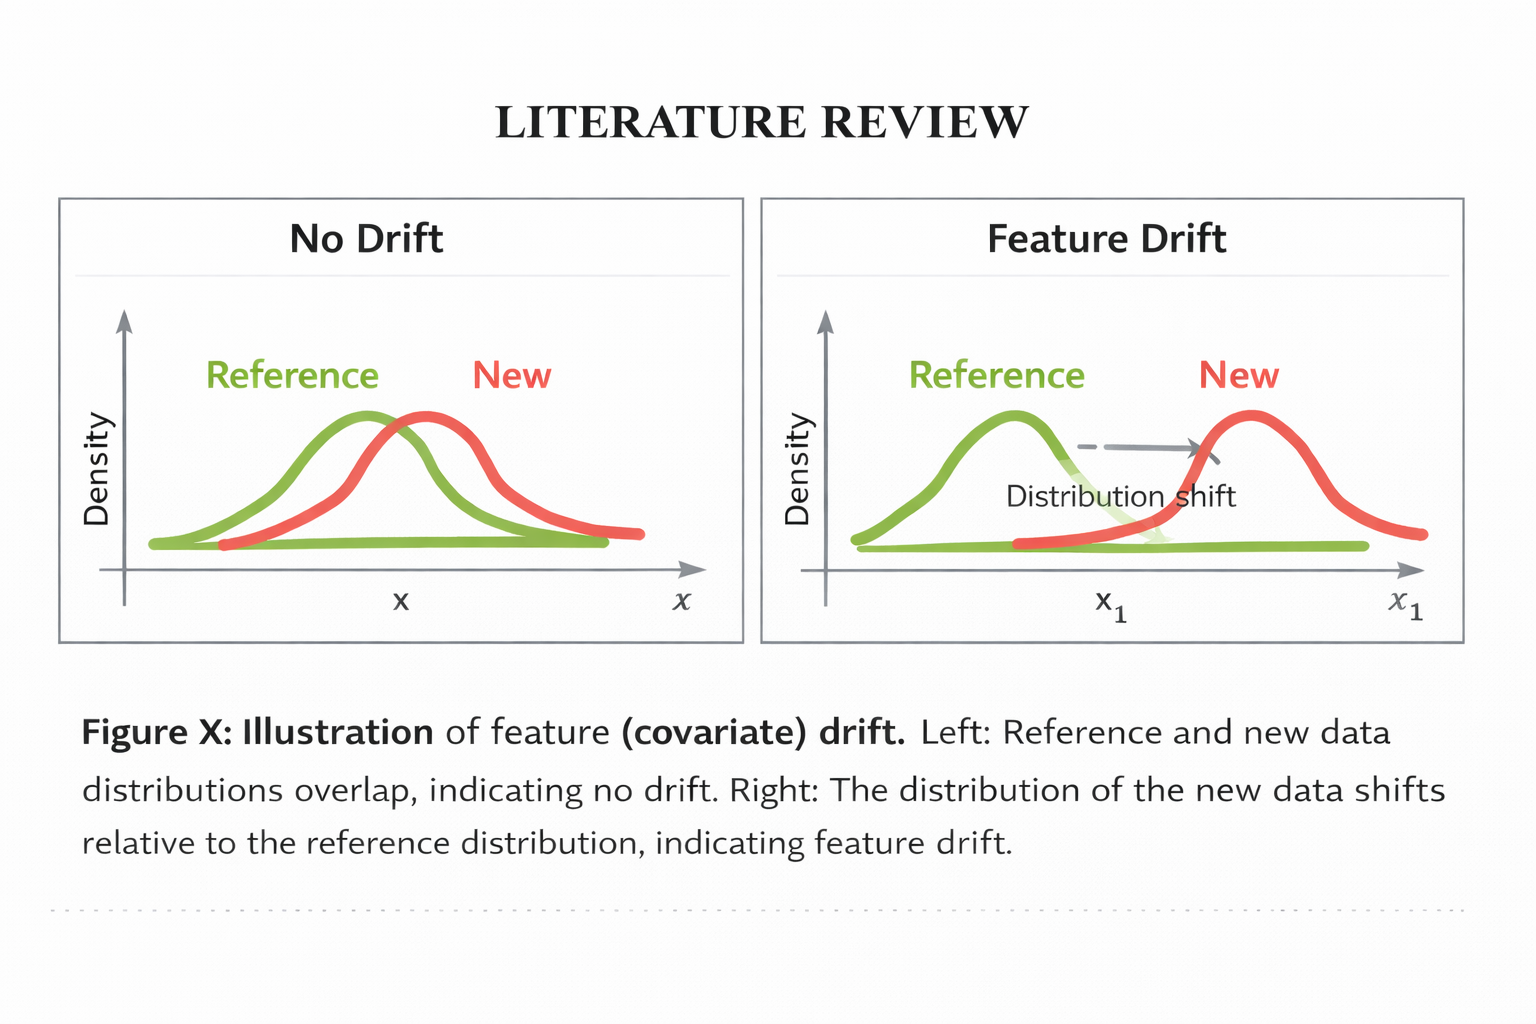
\includegraphics[width=.95\textwidth,keepaspectratio]{figures/figure-1.png}
    \caption{Comparison of no drift versus drift scenarios. Left: When distributions overlap, the adversarial classifier cannot distinguish data sources (AUC $\approx$ 0.5). Right: When drift occurs, distributions shift and the classifier can distinguish sources (AUC $>>$ 0.5).}
    \label{fig:feature-drift}
\end{figure}

\section{Overview}
Drift detection addresses the challenge that arises when the statistical characteristics of data evolve over time in a manner that impacts the validity of a machine learning model \citep{Lu2018, Gama2014}. According to \citet{Bayram2022}, when users, environments, data sources, or the relationships between labels and features change, model accuracy can diminish. \citet{Gama2014} and \citet{Sculley2015} emphasize that drift detection identifies such modifications early, allowing practitioners to adapt, retrain, or update the model accordingly. A robust understanding of drift types and detection methods is essential for designing effective monitoring systems.

\section{Types of Drift}
Drift can be categorized along two main dimensions: by the nature of the change (what component of the data-generating process is affected) and by the temporal pattern of the change (how the drift manifests over time) \citep{Lu2018, Gama2014}.

\subsection{Drift by Nature of Change}
Based on which component of the joint distribution $P(X, y)$ changes, the literature \citep{Lu2018, Gama2014, Tsymbal2004} classifies drift into the following types:

\textbf{Concept Drift (Real Drift):} The conditional distribution $P(y|X)$ changes over time while the feature distribution $P(X)$ may or may not change \citep{Lu2018, Zliobaite2010}. This represents a change in the underlying relationship between inputs and outputs---the ``concept'' the model has learned becomes invalid. For example, the factors that determine creditworthiness may evolve due to economic shifts, even if the applicant characteristics (features) remain similar \citep{Gama2014}. Concept drift directly degrades model performance because the learned decision boundaries no longer reflect the true input-output relationship \citep{Lu2018}.

\textbf{Covariate Drift (Feature Drift / Virtual Drift):} The marginal distribution of input features $P(X)$ changes over time while the conditional relationship $P(y|X)$ remains stable \citep{Tsymbal2004, Shimodaira2000}. The ground-truth concept does not change, but the model may encounter inputs outside its training distribution. For example, a fraud detection model trained on transaction patterns from one demographic may receive data from a different user population, even though the definition of fraud remains unchanged \citep{Tsymbal2004}. Covariate drift can degrade model performance because the model is exposed to feature regions where it may not generalize well \citep{Shimodaira2000}.

\textbf{Prior Probability Drift (Label Shift):} The marginal distribution of labels $P(y)$ changes over time while $P(X|y)$ remains stable \citep{Tsymbal2004}. This occurs when the prevalence of different classes changes---for instance, a seasonal increase in a particular disease affecting the class balance in medical diagnosis. This is sometimes called class imbalance shift \citep{Lu2018}.

\textbf{Note on Terminology:} The literature uses varied terminology \citep{Lu2018}. The term ``concept drift'' is sometimes used as an umbrella term for any distribution change affecting model performance \citep{Gama2014}, while some reserve it specifically for changes in $P(y|X)$ \citep{Tsymbal2004}. This thesis focuses primarily on covariate (feature) drift detection, as it enables early warning without requiring labels.

\subsection{Drift by Temporal Pattern}
Based on how drift manifests over time, the literature \citep{Lu2018, Gama2014, Zliobaite2010} categorizes drift as follows:

\begin{itemize}
    \item \textbf{Abrupt (Sudden) Drift:} A rapid, discrete change where the data distribution shifts quickly from one state to another within a short time period \citep{Gama2014}.
    
    \item \textbf{Gradual Drift:} A new distribution progressively replacing the old one over an extended duration, with samples from both distributions interleaved during the transition period \citep{Lu2018}.
    
    \item \textbf{Incremental Drift:} Small but continuous changes accumulating over time, eventually resulting in a significant distributional shift \citep{Zliobaite2010}.
    
    \item \textbf{Recurring (Seasonal) Drift:} Previously observed distributions reappearing periodically due to cyclical patterns, such as seasonal effects in retail or recurring user behavior patterns \citep{Lu2018, Gama2014}.
\end{itemize}

Understanding drift patterns is important for detector design: abrupt drift requires rapid response, gradual drift requires sustained sensitivity, and recurring drift benefits from mechanisms that can recognize previously seen distributions \citep{Gama2014}.

\section{Classification of Drift Detection Methods}
Based on comprehensive surveys of drift detection literature \citep{Lu2018, Gama2014, Tsymbal2004, Hinder2024}, drift detection methods can be classified by multiple dimensions. According to \citet{Lu2018}, the most fundamental distinction is based on label availability: whether the method requires access to ground-truth labels (supervised) or operates without them (unsupervised).

\subsection{Supervised Drift Detection Methods}
According to \citet{Gama2014} and \citet{Gama2004}, supervised drift detection methods require access to ground-truth labels and primarily monitor model performance or prediction errors to detect distributional changes. \citet{Gama2004} and \citet{BaenaGarcia2006} explain that these methods operate under the assumption that unexpected changes in error characteristics---such as increases in error rate, loss magnitude, variance, or cumulative deviation---are indicative of underlying drift.

Key supervised drift detection algorithms include:

\textbf{Drift Detection Method (DDM):} According to \citet{Gama2004}, DDM monitors the online error rate and its standard deviation. When these statistics exceed predefined thresholds derived from binomial distribution bounds, DDM signals a warning or drift state. \citet{Gama2004} note that DDM is effective for abrupt drift but may be slow to detect gradual changes.

\textbf{Early Drift Detection Method (EDDM):} EDDM extends DDM by tracking the distance between consecutive classification errors rather than just the error rate \citep{BaenaGarcia2006}. This modification improves sensitivity to gradual drift by detecting when errors cluster more closely together.

\textbf{Page--Hinkley Test:} This sequential analysis technique uses cumulative sums to detect changes in the mean of a monitored signal \citep{Page1954}. When cumulative deviation exceeds a threshold, drift is indicated.

\textbf{Hoeffding Drift Detection Methods (HDDM-A, HDDM-W):} These methods use Hoeffding's inequality to provide statistically grounded drift decisions with theoretical guarantees \citep{FriasBlanco2015}. HDDM-A detects abrupt changes using moving averages, while HDDM-W is designed for gradual drift using window-based statistics.

\textbf{Limitations:} Supervised methods fundamentally require labeled data, which may be delayed, expensive, or unavailable in many production scenarios \citep{Lu2018, Sethi2017}. They also react to drift after it has already caused performance degradation, rather than detecting distributional change proactively.

\subsection{Unsupervised Drift Detection Methods}
Unsupervised drift detection methods do not require ground-truth labels and instead monitor changes in data distribution, model outputs, or internal representations \citep{Tsymbal2004, Hinder2024}. These methods enable earlier detection of distributional shifts---before performance degradation becomes observable---making them particularly valuable in production environments with label delays \citep{Sethi2017}.

\subsubsection{Statistical Distribution-Based Methods}
Statistical test--based methods detect drift by directly examining changes in data distributions through hypothesis testing or distance-based measures \citep{Rabanser2019, Raab2020}. A common strategy compares a reference data window against a current data window to test whether they originate from the same distribution \citep{BifetGavalda2007}.

Key statistical drift detection methods include:

\textbf{Adaptive Windowing (ADWIN):} ADWIN dynamically maintains a sliding window and automatically shrinks it when statistically significant distributional change is detected \citep{BifetGavalda2007}. It provides theoretical guarantees on false positive and false negative rates and adapts its window size based on observed change.

\textbf{KSWIN:} This method applies the Kolmogorov--Smirnov two-sample test over sliding windows to detect changes in one-dimensional feature distributions \citep{Raab2020}. KSWIN is non-parametric and makes minimal assumptions about the data distribution.

\textbf{Chi-Squared Test-Based Detectors:} These use the chi-squared test to compare categorical feature distributions or discretized continuous features between time periods \citep{Lu2018}.

\textbf{Kullback--Leibler (KL) Divergence and Other Divergence Measures:} Methods that quantify the ``distance'' between probability distributions, including KL divergence, Jensen--Shannon divergence, and Hellinger distance, can all be used to measure distributional shift \citep{Dasu2006}.

\textbf{Maximum Mean Discrepancy (MMD):} MMD is a kernel-based two-sample test that compares distributions by mapping them into a reproducing kernel Hilbert space, capable of capturing complex multivariate distributional differences \citep{Gretton2012}.

\textbf{Strengths and Limitations:} Statistical tests are interpretable, theoretically grounded, and label-free \citep{Rabanser2019}. However, they can be sensitive to noise (causing false alarms), may struggle in high-dimensional spaces due to the curse of dimensionality, and typically test marginal distributions rather than joint distributions \citep{Lu2018, Webb2016}.

\textbf{Comparison of Statistical Methods with Adversarial Validation:}

Table~\ref{tab:method-comparison} compares popular univariate statistical methods (PSI, KS) with the multivariate Adversarial Validation approach used in this thesis.

\begin{table}[!htbp]
\centering
\caption{Comparison of Drift Detection Approaches}
\label{tab:method-comparison}
\begin{tabular}{p{2.5cm}p{4cm}p{4cm}p{3cm}}
\hline
\textbf{Method} & \textbf{Approach} & \textbf{Strengths} & \textbf{Limitations} \\
\hline
\textbf{PSI (Population Stability Index)} & Compares binned distributions of single features; PSI $> 0.25$ indicates significant drift & Simple, interpretable, industry standard & Univariate only; requires binning; misses feature correlations \\
\hline
\textbf{KS Test (Kolmogorov-Smirnov)} & Non-parametric test comparing cumulative distributions per feature & No distributional assumptions; exact p-values & Univariate only; multiple testing problem with many features \\
\hline
\textbf{Adversarial Validation} & Trains classifier to distinguish old vs. new data; uses AUC as drift signal & Multivariate; captures feature interactions; single unified test & Requires classifier training; no built-in explainability (addressed by EADD) \\
\hline
\end{tabular}
\end{table}

The key distinction is that PSI and KS are \textbf{univariate} methods---they test each feature independently. When monitoring $d$ features, this requires $d$ separate tests, leading to the ``false alarm storm'' problem where the probability of at least one false positive increases with $d$. Adversarial Validation is inherently \textbf{multivariate}, testing the joint distribution $P(X_1, X_2, \ldots, X_d)$ in a single unified check.

\subsubsection{Model-Based Discriminative Methods}
According to \citet{Pan2020}, \citet{LopezPazOquab2017}, and \citet{Sethi2017}, discriminative drift detection methods train an auxiliary model to distinguish between reference and current data distributions. \citet{LopezPazOquab2017} explain that the core idea is to frame drift detection as a classification problem: if a classifier can accurately predict whether each instance originates from the reference or current distribution, the distributions must be distinguishably different.

Key approaches include:

\textbf{Domain Classifier / Adversarial Validation:} According to \citet{Pan2020} and \citet{Qian2021}, this approach trains a binary classifier (e.g., logistic regression, random forest, gradient boosting) to discriminate samples from reference vs. current windows. \citet{Pan2020} note that high discriminative performance (measured by accuracy, AUC, or similar metrics) indicates significant distributional shift.

\textbf{Discriminative Drift Detector (D3):} \citet{Gozuacik2019} developed this unsupervised method that trains a classifier (logistic regression) to distinguish between old and new data windows, using AUC as the drift signal. D3 has demonstrated strong performance in recent benchmarks \citep{Lukats2025} and represents the state-of-the-art in discriminative drift detection.

\textbf{Margin Density Drift Detection (MD3):} \citet{Sethi2017} proposed an alternative approach that monitors margin density---the proportion of samples near the decision boundary---to detect drift without requiring true labels.

\textbf{Margin-Based and Density-Based Discriminators:} According to \citet{DitzlerPolikar2011}, these methods monitor changes in classifier margin densities or decision boundary proximity to detect distributional shifts.

\textbf{Strengths:} Discriminative methods can capture high-dimensional, non-linear distributional shifts that marginal univariate tests may miss \citep{LopezPazOquab2017}. They require no labels for the drift detection task itself (only pseudo-labels indicating data source) and naturally aggregate information across all features \citep{Pan2020}.

\textbf{Limitations:} These methods require training a classifier at each monitoring step, which has computational cost; performance depends on classifier choice and hyperparameters; and interpretation of drift signals may be less intuitive than statistical test p-values \citep{Sethi2017}.

\subsubsection{Representation-Based Methods}
Representation-based methods detect drift by monitoring changes in learned representations or embeddings rather than raw feature distributions \citep{Rabanser2019, Liu2020}:

\textbf{Embedding Distribution Shift:} Computing statistical distances (cosine similarity, Wasserstein distance, MMD) between reference and current embedding distributions derived from neural network intermediate layers \citep{Rabanser2019}.

\textbf{Deep Learning Representation Monitoring:} This approach tracks stability of learned representations across time, leveraging insights from domain adaptation and transfer learning literature \citep{Long2016}.

These methods are particularly relevant for deep learning systems where raw feature distributions may not reflect semantically meaningful changes \citep{Liu2020}.

\subsubsection{Prediction-Based / Output-Based Methods}
Prediction-based methods detect drift by monitoring changes in model outputs over time without requiring evaluation of prediction correctness \citep{Sethi2017, Gozuacik2019}:

\textbf{Prediction Distribution Shift:} Monitoring changes in the distribution of model predictions (class probabilities, regression outputs) over time \citep{Gozuacik2019}.

\textbf{Uncertainty / Entropy Monitoring:} Tracking prediction entropy or uncertainty scores under the assumption that rising uncertainty reflects exposure to out-of-distribution data \citep{Guo2017}.

\textbf{Confidence Monitoring:} Tracking changes in model confidence levels and softmax output distributions \citep{Guo2017}.

\textbf{Limitations:} These methods depend on model calibration. If the model is poorly calibrated---which is common for modern deep learning models---changes in confidence may not reliably indicate drift \citep{Guo2017, Ovadia2019}.

\subsubsection{State-of-the-Art Unsupervised Detectors (2019--2025)}
Recent benchmarking by \citet{Lukats2025} provides a systematic evaluation of fully unsupervised drift detectors on real-world data streams. Their study tested numerous algorithms and identified seven that function reliably on messy, real-world data. This survey represents a critical ``reality check'' for the field, demonstrating that detecting change without ground-truth labels is possible but fragile.

\textbf{D3 (Discriminative Drift Detector):} According to \citet{Gozuacik2019}, D3 trains a logistic regression classifier to distinguish between old and new data windows, using AUC as the drift signal. \citet{Lukats2025} found D3 to be the overall winner---the most robust and accurate across different data types. However, D3 remains a ``black box'': it signals \textit{that} drift occurred but provides no insight into \textit{which} features drifted or \textit{why}.

\textbf{CSDDM (Clustered Statistical Drift Detection Method):} According to \citet{CSDDM2021}, this method uses PCA for dimensionality reduction followed by K-Means clustering, then applies statistical tests to detect cluster shifts. \citet{Lukats2025} report it performed exceptionally well on the ``lift-per-drift'' metric, catching drifts with minimal false alarms.

\textbf{SPLL (Semi-Parametric Log-Likelihood):} \citet{SPLL2013} developed this approach that fits probability density models to reference data and detects drift when new observations have anomalously low likelihood under the learned distribution. It is effective for sudden drift patterns.

\textbf{IBDD (Image-Based Drift Detector):} According to \citet{IBDD2020}, this creative approach converts numerical data streams into images and applies image comparison techniques to detect distributional changes. While highly accurate, \citet{Lukats2025} note it can be biased by its frequent reset strategy.

\textbf{OCDD (One-Class Drift Detector):} \citet{OCDD2021} proposed using one-class SVMs to define ``normal'' data boundaries and flag drift when incoming data falls outside these boundaries. While sound in principle, D3 generally outperformed OCDD in benchmarks \citep{Lukats2025}.

\textbf{NN-DVI (Nearest Neighbor Density Variation):} According to \citet{NNDVI2018}, this method monitors changes in local data density by tracking nearest-neighbor distances. Drift is signaled when density patterns shift significantly. It performs well for gradual density changes but can be sensitive to noise.

\textbf{UCDD (Unsupervised Concept Drift Detection):} \citet{UCDD2020} developed a clustering-based approach that assigns pseudo-labels based on cluster membership and monitors boundary shifts. It serves as a reliable baseline in unsupervised drift detection.

\textbf{BNDM (Bayesian Non-parametric Drift Monitor):} This method uses a Pólya tree test to detect distributional changes without parametric assumptions. However, \citet{Lukats2025} report that BNDM struggled with small sample sizes in their benchmark, limiting its practical applicability in streaming scenarios where window sizes are constrained.

\textbf{UDetect (Univariate Detection):} This approach monitors standard deviation changes using Shewhart control charts. While simple and computationally efficient, \citet{Lukats2025} found it had a high failure rate (45\%) in their benchmark, making it unreliable for production deployment.

\textbf{Industrial Drift Detection Libraries:}
Beyond research algorithms, several industrial libraries provide production-ready drift detection:
\begin{itemize}
    \item \textbf{Alibi Detect}: Open-source Python library (by Seldon) implementing multivariate drift detection via Kolmogorov--Smirnov tests, MMD, and learned kernel methods.
    \item \textbf{NannyML}: Open-source library providing Confidence-Based Performance Estimation (CBPE) for monitoring model performance without ground-truth labels.
    \item \textbf{Evidently AI}: Open-source ML monitoring framework with built-in statistical drift tests for tabular data.
\end{itemize}

\textbf{Gap Identified from Benchmark Analysis:} While these libraries and algorithms exist, according to \citet{Lukats2025}, they share a common limitation: they typically report only \textit{whether} drift occurred, not \textit{where} or \textit{why}. Statistical libraries often run separate univariate tests for each feature, causing ``false alarm storms'' when many features are monitored simultaneously. Although \citet{LopezPazOquab2017} proposed the classifier two-sample test (C2ST) framework with principled significance testing, existing streaming implementations such as D3 \citep{Gozuacik2019} use only fixed AUC thresholds and discard the learned classifier without exploiting it for explainability. The field lacks an integrated method that combines a statistically rigorous multivariate check with granular, feature-level explanations of drift sources.

\subsection{Hybrid and Ensemble Methods}
Hybrid approaches integrate multiple sources of information---both supervised and unsupervised signals---to improve drift detection robustness \citep{Gama2014, Krawczyk2017}:

\textbf{Context-Aware Drift Detection:} Combining model predictions, user context, operational signals, and metadata to compute context-weighted drift scores \citep{Krawczyk2017}.

\textbf{Multi-Signal Ensemble Methods:} Integrating predictions, embeddings, operational KPIs, and metadata into a unified drift score \citep{Krawczyk2017}.

\textbf{Drift Detection Ensembles:} Combining multiple base detectors using voting, weighting, or meta-learning to reduce both false alarms and missed detections \citep{Krawczyk2017}.

\section{Limitations of Existing Methods}
While the drift detection literature offers diverse approaches, each category has characteristic limitations:

\textbf{Supervised Methods (DDM, EDDM, HDDM):} These require timely labeled data, which is often delayed or unavailable in production \citep{Lu2018}. They detect drift reactively---only after performance degradation has already occurred \citep{Sethi2017}.

\textbf{Statistical Distribution Methods (ADWIN, KSWIN, KL-Divergence):} These can be sensitive to noise, leading to false alarms \citep{Rabanser2019}. They may struggle in high-dimensional or correlated feature spaces and typically test marginal distributions, potentially missing joint distribution changes \citep{Lu2018, Webb2016}.

\textbf{Prediction/Uncertainty-Based Methods:} These rely on model calibration. Modern ML models are often poorly calibrated, especially under distribution shift, causing these signals to be unreliable \citep{Guo2017, Ovadia2019}.

\textbf{Context-Aware Methods:} These require pre-specification of relevant context variables, which may be incomplete, noisy, or themselves drift over time \citep{Krawczyk2017}. Misspecified context can cause missed detections or spurious alarms.

\textbf{Fundamental Gap:} Critically, most existing methods do not directly test whether new data is statistically distinguishable from historical data in the original feature space \citep{LopezPazOquab2017}. Discriminative approaches offer a natural, model-agnostic signal of drift that does not depend on predefined contexts, labels, or calibrated uncertainties---yet this perspective has received limited systematic attention in the drift detection literature \citep{Pan2020}.

This thesis aims to bridge this gap by establishing adversarial validation as a viable, general-purpose drift detection technique through rigorous empirical evaluation and practical methodology development.

\section{Related Work: Adversarial Validation}

\subsection{Concept and Origins}
According to \citet{Pan2020}, adversarial validation was originally proposed as a practical technique for diagnosing dataset shift between training and evaluation data. \citet{Pan2020} and \citet{Qian2021} explain that the approach reframes the comparison of two datasets as a binary classification problem: train a classifier to predict whether each instance originates from the reference distribution (e.g., training data) or the target distribution (e.g., test or new data). \citet{LopezPazOquab2017} note that high discriminative performance indicates statistical separability---hence significant distributional shift---while near-random performance suggests the datasets are largely indistinguishable.

According to \citet{Pan2020}, the term ``adversarial'' reflects the insight that if an adversary (the classifier) cannot distinguish the data sources, the distributions must be similar. \citet{LopezPazOquab2017} note this is related to the discriminator component in Generative Adversarial Networks (GANs), though applied here for diagnostic rather than generative purposes.

\subsection{Industrial Applications}
\textbf{Uber's MaLTA System:} \citet{Pan2020} presented adversarial validation at Uber for their MaLTA (Machine Learning Targeting Automation) user targeting system. They trained a classifier to distinguish historical training data from newly observed targeting data. When the adversarial classifier exhibited strong separability, it signaled train-deployment mismatch, prompting feature filtering and retraining adjustments before deployment. Their results demonstrated improved robustness compared to naive retraining strategies that react only after observable performance degradation.

\textbf{Credit Scoring:} \citet{Qian2021} applied adversarial validation to manage dataset shift in credit scoring. They trained an adversarial classifier to distinguish historical credit applications from recent ones, using the classifier's predictions to filter training samples---keeping only those most similar to the current deployment distribution for model training.

\textbf{Image Classification and Operations:} Additional applications include using adversarial validation to quantify dataset complexity in image classification \cite{RenzaMoyaAlbor2024} and to detect when historical data is no longer representative in manufacturing/operations settings \cite{Senoner2023}.

\textbf{Feature Attribution Monitoring at Google:} In an industry report, \citet{TalySato2021} described how Google's Vertex AI platform uses feature attribution monitoring to detect model degradation in production. Their system computes feature attribution baselines during model training and continuously compares production attributions against these baselines, alerting engineers with diagnostic information about which features changed. According to the report, this approach detected a service degradation incident that traditional input-distribution monitoring missed, because the drift manifested in feature importance patterns rather than in raw input statistics. While this is industry-reported evidence rather than peer-reviewed research, the deployment at Google scale suggests that feature-level attribution analysis can provide superior drift diagnostics compared to aggregate distribution tests.

\textbf{Cloud Industry Standardization:} The necessity of feature attribution monitoring is rapidly becoming an industry standard across major cloud providers. As with Google's Vertex AI, Amazon Web Services (AWS) has integrated ``Feature Attribution Drift'' monitoring into Amazon SageMaker Clarify \citep{AWSSageMaker2025}. SageMaker automatically calculates a SHAP baseline during training and actively monitors production data for deviations in these attribution scores. This cross-platform adoption by leading cloud providers validates the core premise of EADD: MLOps drift detection is increasingly moving toward continuous, explainable feature attribution rather than basic distribution tracking.

\section{Gap in the Literature}
While discriminative methods like D3 have proven that adversarial validation can accurately detect drift \citep{Gozuacik2019, Lukats2025}, and \citet{LopezPazOquab2017} have established the theoretical foundation for classifier-based two-sample testing with significance calibration, significant gaps remain that limit practical utility in production MLOps environments:

\begin{enumerate}
    \item \textbf{The ``Black Box'' Problem:} According to \citet{Lukats2025}, existing discriminative detectors like D3 signal \textit{that} drift occurred but provide no insight into \textit{which} features drifted or \textit{why}. In complex ML systems, knowing that drift happened is insufficient---engineers need to understand \textit{what drifted} to take appropriate corrective action.
    
    \item \textbf{No Root Cause Analysis:} Current methods provide only a binary detection signal without identifying the specific source of the change \citep{Lukats2025, Gemaque2020}. Production systems require diagnostic capabilities that pinpoint drift sources and guide remediation.
    
    \item \textbf{False Alarm Storm Problem:} Industrial libraries often run separate univariate tests for each feature, causing multiple simultaneous alerts when features are correlated \citep{Rabanser2019}. This overwhelms operators rather than guiding them toward the actual drift source.
    
    \item \textbf{Threshold Calibration Challenges:} According to \citet{Lukats2025}, determining appropriate detection thresholds remains a major challenge. While \citet{LopezPazOquab2017} provide a principled statistical framework for significance testing, existing streaming implementations (D3, OCDD) rely on arbitrary fixed thresholds rather than adopting permutation-based calibration.
    
    \item \textbf{No Actionable Prescriptions:} Even when drift is detected, current methods provide no guidance on appropriate response strategies---whether to retrain fully, adjust specific features, or apply targeted corrections \citep{Bayram2022, Ditzler2015}.
\end{enumerate}

According to recent benchmarks \citep{Lukats2025}, D3 represents the state-of-the-art in detection accuracy. However, its lack of explainability severely limits practical deployment. This thesis proposes \textbf{Explainable Adversarial Drift Detection (EADD)}, which integrates adversarial validation with permutation-based significance testing (adapting the C2ST framework of \citealt{LopezPazOquab2017} for streaming contexts), SHAP-based root cause analysis \citep{Lundberg2017}, and automated remediation prescriptions---transforming drift detection from a binary alarm into an intelligent diagnostic tool.

This thesis aims to bridge this explainability gap by developing a framework that not only detects drift with high accuracy but also provides actionable insights about drift sources and appropriate remediation strategies.


\chapter{Methodology} \label{chap:methodology}

\begin{figure}[!htpb]
    \centering
    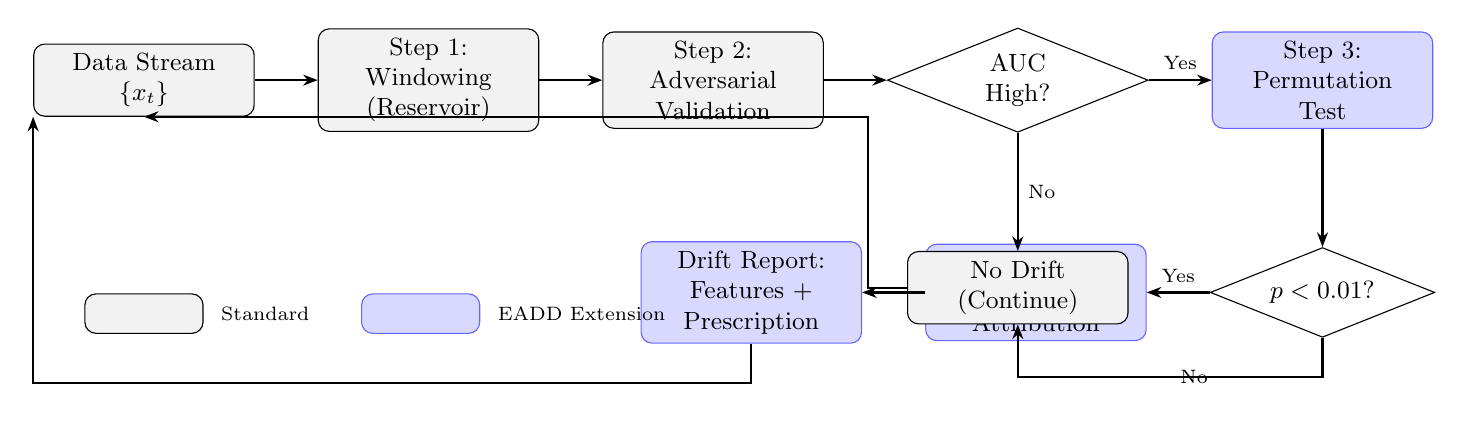
\begin{tikzpicture}[
        node distance=1.2cm and 0.8cm,
        box/.style={rectangle, draw, rounded corners, minimum width=2.8cm, minimum height=0.9cm, align=center, font=\small},
        decision/.style={diamond, draw, aspect=2.5, minimum width=2cm, align=center, font=\small},
        arrow/.style={-{Stealth[scale=0.8]}, thick},
        novel/.style={box, fill=blue!15, draw=blue!60},
        standard/.style={box, fill=gray!10}
    ]
    
    % Step 1: Data Stream
    \node[standard] (stream) {Data Stream\\$\{x_t\}$};
    
    % Step 2: Windowing
    \node[standard, right=of stream] (window) {Step 1:\\Windowing\\(Reservoir)};
    
    % Step 3: Adversarial Classifier
    \node[standard, right=of window] (adv) {Step 2:\\Adversarial\\Validation};
    
    % Decision 1: AUC High?
    \node[decision, right=of adv] (dec1) {AUC\\High?};
    
    % Step 4: Permutation Test (Novel)
    \node[novel, right=of dec1] (perm) {Step 3:\\Permutation\\Test};
    
    % Decision 2: p < 0.01?
    \node[decision, below=1.5cm of perm] (dec2) {$p < 0.01$?};
    
    % Step 5: SHAP (Novel)
    \node[novel, left=of dec2] (shap) {Step 4:\\SHAP Feature\\Attribution};
    
    % Output
    \node[novel, left=of shap] (output) {Drift Report:\\Features +\\Prescription};
    
    % No Drift
    \node[standard, below=1.5cm of dec1] (nodrift) {No Drift\\(Continue)};
    
    % Arrows
    \draw[arrow] (stream) -- (window);
    \draw[arrow] (window) -- (adv);
    \draw[arrow] (adv) -- (dec1);
    \draw[arrow] (dec1) -- node[above, font=\scriptsize] {Yes} (perm);
    \draw[arrow] (dec1) -- node[right, font=\scriptsize] {No} (nodrift);
    \draw[arrow] (perm) -- (dec2);
    \draw[arrow] (dec2) -- node[above, font=\scriptsize] {Yes} (shap);
    \draw[arrow] (dec2.south) -- ++(0,-0.5) -| node[near start, right, font=\scriptsize] {No} (nodrift.south);
    \draw[arrow] (shap) -- (output);
    
    % Loop back
    \draw[arrow] (nodrift.west) -- ++(-0.5,0) |- (stream.south);
    \draw[arrow] (output.south) -- ++(0,-0.5) -| (stream.south west);
    
    % Legend
    \node[standard, minimum width=1.5cm, minimum height=0.5cm] at ($(stream.south)+(0,-2.5)$) (leg1) {};
    \node[right=0.1cm of leg1, font=\scriptsize] {Standard};
    \node[novel, minimum width=1.5cm, minimum height=0.5cm, right=2cm of leg1] (leg2) {};
    \node[right=0.1cm of leg2, font=\scriptsize] {EADD Extension};
    
    \end{tikzpicture}
    \caption{Overview of Explainable Adversarial Drift Detection (EADD) methodology. Blue boxes indicate EADD-specific extensions beyond D3: Permutation Test (Step~3, adapting \citealt{LopezPazOquab2017} for streaming detection) and SHAP Feature Attribution (Step~4). The framework integrates adversarial validation with statistical rigor and root cause analysis.}
    \label{fig:methodology-overview}
\end{figure}

\section{Overview: Explainable Adversarial Drift Detection (EADD)}
This thesis proposes \textbf{Explainable Adversarial Drift Detection (EADD)}, a framework designed specifically for \textbf{Feature Drift} ($P(X)$ shift). The fundamental insight is that \textbf{Adversarial Validation} and \textbf{Feature Drift Detection} are mathematically equivalent---both ask: \textit{``Can a model distinguish between old data and new data based solely on features?''}

While existing methods like D3 \citep{Gozuacik2019} successfully employ adversarial validation to flag distributional changes, and \citet{LopezPazOquab2017} have established the theoretical framework for classifier-based two-sample testing with significance calibration, no prior work has combined these established techniques with post-hoc feature attribution to create an end-to-end explainable drift detection pipeline for streaming data.

EADD integrates three components that collectively address the limitations identified in Chapter~\ref{chap:literature}:
\begin{enumerate}
    \item \textbf{Permutation-Based Statistical Validation:} Adapting the classifier two-sample test framework of \citet{LopezPazOquab2017} to streaming drift detection, replacing D3's fixed AUC threshold with a principled hypothesis test
    \item \textbf{SHAP-Based Root Cause Analysis:} Extracting feature-level drift attribution from the adversarial classifier via TreeSHAP \citep{Lundberg2017}, transforming the binary detection signal into a diagnostic report
    \item \textbf{Automated Prescriptions:} Mapping SHAP importance patterns to actionable MLOps remediation strategies
\end{enumerate}

\section{Problem Formulation}
According to \citet{Pan2020} and \citet{LopezPazOquab2017}, this research formalizes feature (covariate) drift detection as a problem of discriminating between historical reference data and newly arriving observations in a streaming or windowed setting. \citet{Shimodaira2000} explains that the objective is to detect when the underlying feature distribution $P(X)$ changes substantially over time, providing an early indication of distributional drift before observable degradation in task performance occurs.

\textbf{Formal Definition:} Let $\{x_t\}_{t=1}^{T}$ denote a stream of feature vectors arriving over time. At each monitoring point $t$, a drift detector produces a binary decision $d_t \in \{\text{no-drift}, \text{drift}\}$ based on comparison between:
\begin{itemize}
    \item A reference window $W_{ref}$ containing historical samples presumed to represent the stable/baseline distribution
    \item A current window $W_{cur}$ containing the most recent observations under test
\end{itemize}

\textbf{Extended Objective:} Unlike existing detectors that output only a binary drift decision, EADD additionally produces:
\begin{itemize}
    \item A ranked list of features contributing to the drift
    \item Feature importance scores quantifying each feature's contribution
    \item An automated prescription for appropriate remediation action
\end{itemize}

According to \citet{Lu2018} and \citet{Gama2014}, the detection task must balance:
\begin{itemize}
    \item \textbf{Promptness:} Low detection delay (lag between true drift and detection)
    \item \textbf{Reliability:} Low false positive rate (false alarms when no drift exists)
    \item \textbf{Sensitivity:} High true positive rate (detecting drift when it occurs)
    \item \textbf{Efficiency:} Bounded computational and memory requirements suitable for production
    \item \textbf{Explainability:} Clear attribution of drift to specific features (novel contribution)
\end{itemize}

\section{EADD Framework Components}
The EADD methodology maps directly to the thesis requirements:

\begin{table}[!htbp]
\centering
\caption{Alignment of EADD Components with Research Requirements}
\label{tab:eadd-alignment}
\begin{tabular}{p{4.5cm}p{9cm}}
\hline
\textbf{Requirement} & \textbf{EADD Solution} \\
\hline
``Based on Adversarial Validation'' & Step 2: Train classifier to distinguish $W_{ref}$ vs $W_{cur}$ \\
``Based on Permutation Test'' & Step 3: Shuffle labels $B{=}50$ times to calculate p-value \\
``Like D3'' & Foundation: Same discriminative logic, upgraded classifier (LightGBM) \\
``Focus on Feature Drift'' & Step 4: SHAP identifies which $P(X)$ components shifted \\
\hline
\end{tabular}
\end{table}

The methodology consists of four integrated steps:

\textbf{Step 1: Adaptive Reference Windowing} --- Reservoir sampling for representative baseline

\textbf{Step 2: Adversarial Validation (Detector)} --- Train discriminative classifier on $W_{ref}$ vs $W_{cur}$

\textbf{Step 3: Permutation Test (Significance)} --- Statistical validation via label shuffling

\textbf{Step 4: Feature Drift Explainability (SHAP)} --- Identify which features drifted (novel contribution)

\subsection{Step 1: Adaptive Reference Windowing}
To detect Feature Drift, we must compare the current data stream against a stable baseline. EADD maintains two windows consistent with established methodologies \citep{BifetGavalda2007, Tsymbal2004}:

\textbf{Reference Window ($W_{ref}$):} A buffer containing $N_{ref}$ historical samples representing the stable feature distribution $P_{ref}(X)$. Unlike fixed sliding windows that ``forget'' normal data too quickly, EADD uses \textbf{Reservoir Sampling} \citep{Vitter1985} to ensure the reference captures the global distribution of features, not just the most recent batches.

\textbf{Current Window ($W_{cur}$):} A buffer containing the $N_{cur}$ most recent observations representing the current feature distribution $P_{cur}(X)$. As new data arrives, older samples are discarded to maintain responsiveness to recent changes.

\textbf{Update Mechanism:} At each monitoring step:
\begin{itemize}
    \item New samples enter $W_{cur}$
    \item Oldest samples exit $W_{cur}$ 
    \item Reservoir sampling maintains representative $W_{ref}$
    \item Upon confirmed drift, $W_{ref}$ may be reset to current distribution
\end{itemize}

According to \citet{Lu2018}, window sizes represent a bias-variance tradeoff: larger windows provide more stable estimates but slower response; smaller windows enable faster detection but higher variance.

\subsection{Step 2: Adversarial Validation (The Detector)}
This step implements the core \textbf{Adversarial Validation} logic that forms the foundation of both D3 \citep{Gozuacik2019} and EADD. The insight is that Feature Drift detection reduces to a binary classification problem: \textit{can a model tell the difference between old and new data?}

\textbf{Construct Binary Classification Dataset:}
\begin{itemize}
    \item Label all samples from $W_{ref}$ as class 0 (``old'' / reference)
    \item Label all samples from $W_{cur}$ as class 1 (``new'' / current)
    \item Combined dataset: $X = W_{ref} \cup W_{cur}$, $y = \{0\}^{N_{ref}} \cup \{1\}^{N_{cur}}$
\end{itemize}

\textbf{Train Adversarial Classifier:}
Train a binary classifier $f_\theta$ to predict data source from features alone. EADD uses \textbf{LightGBM} \citep{Ke2017} as the default classifier.

\textit{Why LightGBM over D3's Logistic Regression?} D3 \citep{Gozuacik2019} uses logistic regression, which is linear. LightGBM captures \textbf{non-linear feature interactions}, enabling detection of complex Feature Drifts where multiple features shift in correlated ways that linear models miss.

\textbf{Measure Discriminative Performance:}
Evaluate classifier performance using stratified cross-validation:
\begin{itemize}
    \item \textbf{AUC-ROC:} Primary metric---Area under the ROC curve
    \item AUC $\approx$ 0.5: Classifier cannot distinguish $W_{ref}$ from $W_{cur}$ $\rightarrow$ \textbf{No Feature Drift}
    \item AUC $>>$ 0.5: Classifier separates windows $\rightarrow$ $P_{ref}(X) \neq P_{cur}(X)$ $\rightarrow$ \textbf{Feature Drift detected}
\end{itemize}

\textbf{Objective:} If the adversarial classifier achieves high AUC, the feature distributions $P(X)$ have diverged---this is the definition of Feature Drift.

\subsection{Step 3: Statistical Significance via Permutation Test}
A raw AUC score (e.g., 0.65) is inconclusive, as it may reflect genuine distributional change or statistical noise. D3 \citep{Gozuacik2019} and standard adversarial validation approaches \citep{Pan2020} rely on fixed thresholds (e.g., AUC $> 0.7$), which lack principled justification and are sensitive to dataset characteristics. \citet{LopezPazOquab2017} proposed the classifier two-sample test (C2ST) framework, which provides a principled significance testing approach using the binomial null distribution. EADD adapts this framework for streaming drift detection by implementing a \textbf{Permutation Test} \citep{LopezPazOquab2017} that constructs a data-specific null distribution at each monitoring step.

\textbf{The Permutation Test Procedure:}
\begin{enumerate}
    \item \textbf{Generate Null Distribution:} Randomly shuffle the labels (0 and 1) of the combined dataset $B=50$ times
    \item \textbf{Retrain:} For each permutation, retrain the adversarial classifier and compute AUC
    \item \textbf{Build Null:} The $B$ permuted AUCs form the ``Null Distribution'' of AUC scores where \textit{no drift exists}
    \item \textbf{Compare:} Compare the \textit{actual} adversarial AUC against this Null Distribution
\end{enumerate}

\textbf{Drift Confirmation Rule:}
\begin{itemize}
    \item Compute empirical p-value: $p = \frac{\#\{\text{AUC}_{perm} \geq \text{AUC}_{actual}\}}{B}$
    \item Drift is confirmed \textbf{only} if $p < 0.01$ (99th percentile)
\end{itemize}

\textbf{Benefit:} This prevents false alarms caused by small sample sizes or random fluctuations---a common failure mode in standard adversarial validation. The permutation test provides statistical guarantees that the detected drift is real, not noise.

\subsection{Step 4: Feature Drift Explainability via SHAP}
Once the Permutation Test confirms drift (p $<$ 0.01), the next objective is to determine \textit{which features drifted}. This is the core contribution of EADD relative to prior discriminative detectors. A key limitation of D3 \citep{Gozuacik2019} is that it discards the trained classifier after computing AUC. However, the adversarial classifier has already learned to discriminate between the two distributions, encoding precisely \textit{which} features differentiate the reference data from the current data.

\textbf{The SHAP Extraction Method:}
EADD applies \textbf{SHAP (SHapley Additive exPlanations)} \citep{Lundberg2017} to the adversarial classifier:
\begin{enumerate}
    \item Compute SHAP values using TreeSHAP (efficient for LightGBM)
    \item Calculate mean absolute SHAP value per feature: $\text{Importance}_i = \frac{1}{n} \sum_{j=1}^{n} |\text{SHAP}_{ij}|$
    \item Normalize to percentages: $\text{Contribution}_i = \frac{\text{Importance}_i}{\sum_k \text{Importance}_k} \times 100\%$
    \item Rank features by contribution
\end{enumerate}

\textbf{Interpretation---The Core Insight:}
\begin{quote}
A feature with a high SHAP value is a feature that \textbf{heavily helped the model distinguish ``new'' data from ``old'' data}. Therefore: \textbf{High SHAP = High Feature Drift}.
\end{quote}

\textbf{Output Format:}
The system outputs a ranked list of ``Drifting Features'' with contribution percentages:
\begin{itemize}
    \item Example: ``Drift Detected (AUC=0.85, p$<$0.01). Primary Driver: \textbf{Age} (contribution: 45\%), Secondary Driver: \textbf{Income} (contribution: 25\%), Other: Location (15\%), Tenure (10\%), Balance (5\%)''
\end{itemize}

This transforms the drift detector from a binary alarm into an \textbf{intelligent diagnostic tool} that pinpoints exactly which features require attention.

\textbf{Theoretical Justification for Attribution over Distribution:}
The choice of SHAP-based feature attribution over traditional distribution-based monitoring is supported by industry adoption. Google's Vertex AI platform reportedly uses feature attribution monitoring that detected model degradation missed by input-distribution monitoring alone \citep{TalySato2021}, and AWS SageMaker Clarify \citep{AWSSageMaker2025} integrates SHAP-based attribution drift monitoring as a standard capability. This convergence across major platforms suggests attribution-based approaches capture model-relevant drift more effectively. Specifically:
\begin{enumerate}
    \item \textbf{Attribution captures model-relevant drift:} Distribution tests may flag statistically significant but model-irrelevant changes, while attribution methods focus on changes that actually affect model predictions.
    \item \textbf{Attribution provides actionable diagnostics:} Knowing which features' \textit{importance} changed (rather than which features' distributions shifted) directly maps to remediation actions.
    \item \textbf{Attribution handles feature interactions:} SHAP values account for feature interactions through the Shapley value framework, capturing multivariate drift patterns that univariate tests miss.
\end{enumerate}

\subsection{Automated Drift Prescription}
Beyond diagnosis, EADD provides actionable remediation recommendations based on the drift pattern identified:

\textbf{Scenario A: Univariate Drift (Single Feature Dominant)}

\textit{Condition:} One feature contributes $>$50\% of total importance.

\textit{Prescription:} ``Univariate drift detected on [Feature]. Recommended actions:
\begin{itemize}
    \item Investigate data pipeline for [Feature] (sensor failure, data source change)
    \item Consider feature-specific preprocessing adjustment
    \item If persistent: Retrain with reduced weight on [Feature] or exclude temporarily''
\end{itemize}

\textbf{Scenario B: Multivariate Concept Shift (Distributed Importance)}

\textit{Condition:} No single feature exceeds 30\% importance; drift is spread across multiple features.

\textit{Prescription:} ``Multivariate concept shift detected. The entire data structure has changed. Recommended actions:
\begin{itemize}
    \item Full model retraining required immediately
    \item Consider expanding training data to include recent distribution
    \item Review deployment assumptions and feature engineering''
\end{itemize}

\textbf{Scenario C: Feature Subset Drift}

\textit{Condition:} 2-5 features together contribute $>$70\% of importance.

\textit{Prescription:} ``Correlated feature drift detected in [Feature Group]. Recommended actions:
\begin{itemize}
    \item Investigate common data source for affected features
    \item Consider partial retraining with emphasis on affected feature subspace
    \item Evaluate feature engineering for the affected domain''
\end{itemize}

\subsection{Model Adaptation Strategies}
According to \citet{Gama2014}, upon drift detection, the primary prediction model can be adapted:

\textbf{Strategy 1: Drift-Triggered Retraining}
\begin{itemize}
    \item Model is trained at initialization
    \item Retraining occurs only when drift alarm is raised
    \item Reference window resets to current data after retraining
    \item According to \citet{Pan2020}, advantage: Conserves resources; exploits early detection for timely updates
\end{itemize}

\textbf{Strategy 2: Periodic Retraining (Baseline)}
\begin{itemize}
    \item Model is retrained at fixed intervals regardless of drift signals
    \item Advantage: Simple; does not depend on detector reliability
    \item According to \citet{Gama2014}, disadvantage: May retrain unnecessarily or too late
\end{itemize}

\textbf{Strategy 3: Continuous Update with Drift Weighting}
\begin{itemize}
    \item Online learning with sample weighting based on drift score
    \item According to \citet{Krawczyk2017}, recent samples receive higher weights when drift is detected
\end{itemize}

\section{Datasets}
Following the comprehensive benchmark by \citet{Lukats2025}, experiments used both synthetic and real-world data streams to evaluate EADD under controlled and realistic conditions.

\textbf{Synthetic Datasets:}
Custom synthetic data generators were used to create controlled $P(X)$ shifts with known ground-truth drift points, enabling precise measurement of detection delay and accuracy:
\begin{itemize}
    \item \textbf{SineClusters:} Sine-modulated cluster data with controlled drift patterns
    \item \textbf{WaveformDrift2:} Waveform generator with gradual feature drift
    \item \textbf{Custom Generators:} Streams of $n=10{,}000$ samples with $d=5$ features and controlled abrupt, gradual, incremental, and recurring drift injected at known positions (e.g., $t=5{,}000$)
\end{itemize}

\textbf{Real-World Benchmark Datasets:}
Thirteen real-world data streams from the \citet{Lukats2025} benchmark were used, spanning diverse domains and drift characteristics:
\begin{itemize}
    \item \textbf{Electricity (Elec2)} \citep{Harries1999}: 45,312 samples $\times$ 8 features; electricity pricing data with natural market fluctuations
    \item \textbf{INSECTS Variants} \citep{Souza2020}: Six variants---Abrupt Balanced, Gradual Balanced, Incremental Balanced, Incremental-Abrupt Balanced, Incremental-Reoccurring Balanced---each containing $\sim$24,000--80,000 samples $\times$ 33 features with documented ground-truth drift points
    \item \textbf{NOAA Weather:} Weather measurements with temporal drift patterns
    \item \textbf{Outdoor Objects:} Object recognition features with environmental variation
    \item \textbf{Ozone:} Atmospheric ozone level data with seasonal drift
    \item \textbf{Poker Hand:} Card game data with complex feature relationships
    \item \textbf{Powersupply:} Power consumption data with usage pattern changes
    \item \textbf{Rialto Bridge Timelapse:} Image-derived features with temporal variation
    \item \textbf{Luxembourg:} Financial data with market-driven distributional shifts
\end{itemize}

All datasets were processed in streaming fashion, with features used for drift detection. For datasets with known drift points (e.g., INSECTS variants with drift indices at specific sample positions), ground truth was used for computing detection metrics. The INSECTS datasets were particularly valuable as they provide exact drift timestamps, enabling precise measurement of detection delay and false alarm rates.

\section{Baseline Drift Detectors}
EADD was benchmarked against seven state-of-the-art unsupervised drift detectors evaluated in the \citet{Lukats2025} survey, all of which operate without ground-truth labels:

\begin{itemize}
    \item \textbf{D3 (Discriminative Drift Detector)} \cite{Gozuacik2019}: Trains a logistic regression classifier to distinguish old from new data windows, using AUC as the drift signal. Identified as the overall best-performing unsupervised detector in the \citet{Lukats2025} benchmark.
    \item \textbf{BNDM (Bayesian Non-parametric Drift Monitor):} Uses a P\'{o}lya tree test to detect distributional changes without parametric assumptions.
    \item \textbf{CSDDM (Clustered Statistical Drift Detection Method)} \cite{CSDDM2021}: Applies PCA dimensionality reduction followed by K-Means clustering, then uses statistical tests to detect cluster shifts.
    \item \textbf{IBDD (Image-Based Drift Detector)} \cite{IBDD2020}: Converts numerical data streams into images and applies image comparison techniques to detect distributional changes.
    \item \textbf{OCDD (One-Class Drift Detector)} \cite{OCDD2021}: Uses one-class SVMs to define ``normal'' data boundaries and flags drift when incoming data falls outside these boundaries.
    \item \textbf{SPLL (Semi-Parametric Log-Likelihood)} \cite{SPLL2013}: Fits probability density models to reference data and detects drift when new observations have anomalously low likelihood.
    \item \textbf{UDetect (Univariate Detection):} Monitors standard deviation changes using Shewhart control charts.
\end{itemize}

Existing benchmark results for these seven detectors from the \citet{Lukats2025} framework were used for direct comparison with EADD's detection performance across the same datasets.

\section{Evaluation Metrics}

Following \citet{Lu2018}, \citet{Lukats2025}, and \citet{Souza2020}, the following metrics were used to evaluate drift detection performance:

\textbf{Detection Performance Metrics:}
\begin{itemize}
    \item \textbf{Mean Time to Detection (MTD):} Average number of samples between true drift occurrence and detection alarm. Lower is better.
    \item \textbf{Missed Detection Rate (MDR):} Proportion of true drifts that were not detected within a tolerance window. Lower is better.
    \item \textbf{Mean Time between False Alarms (MTFA):} Average number of samples between consecutive false alarms. Higher is better.
    \item \textbf{Mean Time to Recovery (MTR):} Average time for the system to stabilize after drift detection.
    \item \textbf{F1-Score:} Harmonic mean of precision and recall for drift detection decisions.
    \item \textbf{False Positive Rate (FPR):} Proportion of alarms when no drift exists. Lower is better.
\end{itemize}

\textbf{Explainability Metrics:}
\begin{itemize}
    \item \textbf{Feature Attribution Accuracy:} Whether SHAP correctly identifies the ground-truth drifting feature(s) as the top contributor(s).
    \item \textbf{SHAP Dominance Score:} Percentage of total SHAP importance assigned to the true drifting feature(s). Higher indicates more precise attribution.
    \item \textbf{Prescription Accuracy:} Whether the automated prescription matches the actual drift scenario (univariate, subset, or multivariate).
\end{itemize}

\section{Experimental Design}

Four experiments were designed to systematically validate EADD's detection accuracy, explainability, and robustness:

\textbf{Experiment 1: Sensitivity to Temporal Drift Patterns}

Evaluated EADD's ability to detect all four major temporal drift patterns (abrupt, gradual, incremental, recurring) on synthetic data with known ground-truth drift points. Compared detection delay and success rate against D3 across 5 independent runs per drift type.

\textbf{Experiment 2: Real-World Benchmark Comparison}

Benchmarked EADD against seven unsupervised baselines (D3, BNDM, CSDDM, IBDD, OCDD, SPLL, UDetect) across 13 real-world data streams from the \citet{Lukats2025} framework, measuring MTD, MDR, MTR, and overall F1.

\textbf{Experiment 3: Explainability Case Study}

Validated SHAP-based feature attribution accuracy across three controlled synthetic scenarios: (1) univariate drift in a single feature, (2) correlated subset drift across 2--3 features, and (3) multivariate drift distributed across all features. Measured whether EADD correctly identifies drifting features and generates appropriate prescriptions.

\textbf{Experiment 4: Robustness to Stable Data (False Alarm Evaluation)}

Assessed false alarm rates on four types of stable synthetic streams with zero actual drift (Gaussian i.i.d., autocorrelated, heteroscedastic, correlated features). Evaluated EADD's permutation test robustness and compared against D3 at multiple AUC thresholds $\tau \in \{0.6, 0.7, 0.8\}$.

\section{Practical Considerations}

\textbf{Class Imbalance:} When $|W_{ref}| \neq |W_{cur}|$, use:
\begin{itemize}
    \item Stratified cross-validation
    \item Class-weighted classifiers
    \item According to \citet{LopezPazOquab2017}, AUC-ROC rather than accuracy
\end{itemize}

\textbf{Computational Efficiency:}
\begin{itemize}
    \item Use efficient classifiers (logistic regression, small random forests)
    \item Consider approximate methods for large windows
    \item According to \citet{Pan2020}, implement incremental training where possible
\end{itemize}

\textbf{Temporal Leakage Prevention:}
\begin{itemize}
    \item Use purged cross-validation to avoid temporal overlap between folds
    \item According to \citet{Souza2020}, ensure strict temporal ordering in train/test splits
\end{itemize}

\textbf{Threshold Calibration:}
\begin{itemize}
    \item Use validation data with known drift to tune $T_{drift}$
    \item According to \citet{Pan2020}, consider adaptive thresholds based on baseline variance
\end{itemize}


\chapter{Experiments and Results} \label{chap:results}

This chapter presents the experimental evaluation of Explainable Adversarial Drift Detection (EADD). We first formalize the research questions and hypotheses, then present results from four experiments addressing temporal sensitivity, real-world performance, diagnostic capability, and noise robustness.

\section{Research Questions}

Based on the gaps identified in Chapter~\ref{chap:literature}, this thesis investigates three research questions:

\begin{itemize}
    \item \textbf{RQ1 (Detection Accuracy):} Does EADD achieve comparable or superior drift detection performance (F1-score, detection delay) to state-of-the-art unsupervised detectors across synthetic and real-world data streams?
    
    \item \textbf{RQ2 (Explainability):} Can EADD's SHAP-based feature attribution correctly identify the root cause of drift, and does the automated prescription system provide accurate drift categorization?
    
    \item \textbf{RQ3 (Robustness):} Does EADD's permutation test significantly reduce false alarm rates on stable data compared to threshold-based approaches like D3?
\end{itemize}

\section{Hypotheses}

Three formal hypotheses were tested:

\begin{itemize}
    \item \textbf{H1 (Detection Coverage):} EADD detects a broader range of temporal drift patterns than D3. Formally: H1a tests whether EADD detects significantly more drift types (binomial test), and H1b tests whether EADD achieves comparable detection delay where both detectors succeed (Mann--Whitney U test, $\alpha = 0.05$).
    
    \item \textbf{H2 (False Alarm Reduction):} EADD produces significantly fewer false alarms than D3 on stable data. Formally, $H_0$: $\text{FPR}_{\text{EADD}} \geq \text{FPR}_{\text{D3}}$ vs $H_1$: $\text{FPR}_{\text{EADD}} < \text{FPR}_{\text{D3}}$. Tested using the Mann--Whitney U test (one-sided, $\alpha = 0.05$) at multiple D3 threshold settings ($\tau \in \{0.6, 0.7, 0.8\}$).
    
    \item \textbf{H3 (Explainability Accuracy):} EADD correctly identifies the ground-truth drifting feature(s) as the top SHAP contributor in controlled experiments. Evaluated qualitatively across three controlled synthetic scenarios ($\alpha = 0.05$).
\end{itemize}

\section{Experimental Setup}

\textbf{Environment:} Experiments were conducted in Python 3.10 using LightGBM \citep{Ke2017} for the adversarial classifier and SHAP (SHapley Additive exPlanations) for feature attribution \citep{Lundberg2017}. Implementation is available in the \texttt{detectors/eadd.py} module within the \citet{Lukats2025} benchmark framework.

\textbf{EADD Configuration:}
\begin{itemize}
    \item \textbf{Reference Window ($N_{ref}$):} 500 samples
    \item \textbf{Current Window / Step Size ($N_{cur}$):} 200 samples
    \item \textbf{AUC Threshold:} 0.7 (adapted from industry practice \citep{Pan2020})
    \item \textbf{Permutation Test:} $B = 50$ permutations, $\alpha = 0.01$
    \item \textbf{LightGBM:} 30 estimators, learning rate 0.1, max depth $= -1$ (unlimited), 31 leaves
    \item \textbf{Cross-Validation:} Stratified 5-fold within each detection cycle
    \item \textbf{Monitoring Frequency:} Every 50 samples
\end{itemize}

\textbf{D3 Baseline Configuration:}
\begin{itemize}
    \item Logistic regression classifier
    \item Matching window configuration ($N_{ref} = 500$, $N_{cur} = 200$)
    \item AUC threshold of 0.7 (no permutation test)
\end{itemize}

\textbf{Baselines:} EADD was compared against seven unsupervised detectors from the \citet{Lukats2025} benchmark: D3 \citep{Gozuacik2019} (primary comparison), BNDM, CSDDM, IBDD, OCDD, SPLL, and UDetect. All baselines were run with their default configurations as provided in the benchmark framework. A per-detector timeout of 120 seconds was applied for real-world datasets to handle scalability limitations of certain detectors (e.g., BNDM on high-dimensional data).

\section{Experiment 1: Multi-Detector Sensitivity to Temporal Drift Patterns}

\textbf{Objective:} Systematically compare EADD against seven state-of-the-art unsupervised drift detectors across all four major temporal drift patterns---abrupt, gradual, incremental, and recurring---to evaluate the trade-offs between detection speed, missed drift rate, and false alarm rate.

\textbf{Data Generation:}
Synthetic data streams of $n = 10{,}000$ samples with $d = 5$ features were generated for each drift type. Drift was injected at known points as follows:
\begin{itemize}
    \item \textbf{Abrupt:} Instantaneous mean shift of $+2\sigma$ at $t = 5{,}000$
    \item \textbf{Gradual:} Linear interpolation between old and new distributions over 2{,}000 samples
    \item \textbf{Incremental:} Small step increases of $0.1\sigma$ every 200 samples
    \item \textbf{Recurring:} Oscillating between original and shifted distributions with period 2{,}000 (3 drift points)
\end{itemize}

All eight detectors were run under identical conditions with their default configurations from the \citet{Lukats2025} benchmark framework.

\textbf{Baselines:} D3 \citep{Gozuacik2019}, BNDM, CSDDM, IBDD, OCDD, SPLL, and UDetect.

\textbf{Results:}

Table~\ref{tab:exp1-results} presents the detection performance across all eight detectors and four drift types.

\begin{table}[!htbp]
\centering
\caption{Experiment 1: Multi-Detector Comparison on Synthetic Drift Patterns. MTD = Mean Time to Detection (samples); MDR = Missed Detection Rate; FA = False Alarms. ``---'' indicates the detector missed all drift points.}
\label{tab:exp1-results}
\begin{tabular}{l|ccc|ccc|ccc|ccc}
\hline
 & \multicolumn{3}{c|}{\textbf{Abrupt}} & \multicolumn{3}{c|}{\textbf{Gradual}} & \multicolumn{3}{c|}{\textbf{Incremental}} & \multicolumn{3}{c}{\textbf{Recurring}} \\
\textbf{Detector} & MTD & MDR & FA & MTD & MDR & FA & MTD & MDR & FA & MTD & MDR & FA \\
\hline
\textbf{EADD} & 149 & 0.0 & \textbf{0} & 849 & 0.0 & \textbf{0} & 749 & 0.0 & \textbf{1} & 182 & 0.0 & \textbf{0} \\
D3 & \textbf{98} & 0.0 & 0 & --- & 1.0 & --- & --- & 1.0 & --- & 157 & 0.0 & 0 \\
BNDM & 272 & 0.0 & 4 & \textbf{26} & 0.0 & 6 & 383 & 0.0 & 6 & 219 & 0.0 & 3 \\
CSDDM & 206 & 0.0 & 5 & 413 & 0.0 & 6 & \textbf{9} & 0.0 & 5 & 84 & 0.0 & 6 \\
IBDD & \textbf{18} & 0.0 & 41 & 153 & 0.0 & 48 & 156 & 0.0 & 47 & \textbf{11} & 0.0 & 49 \\
OCDD & 249 & 0.0 & 18 & 249 & 0.0 & 18 & 249 & 0.0 & 18 & 249 & 0.0 & 16 \\
SPLL & 66 & 0.0 & 0 & --- & 1.0 & --- & --- & 1.0 & --- & 72 & 0.0 & 0 \\
UDetect & --- & 1.0 & --- & --- & 1.0 & --- & --- & 1.0 & --- & --- & 1.0 & --- \\
\hline
\end{tabular}
\end{table}

Figure~\ref{fig:heatmap-synthetic} presents heatmaps of detection performance across all detector--drift-type combinations, providing a visual summary of Table~\ref{tab:exp1-results}.

\begin{figure}[!htbp]
    \centering
    \begin{minipage}{0.48\textwidth}
        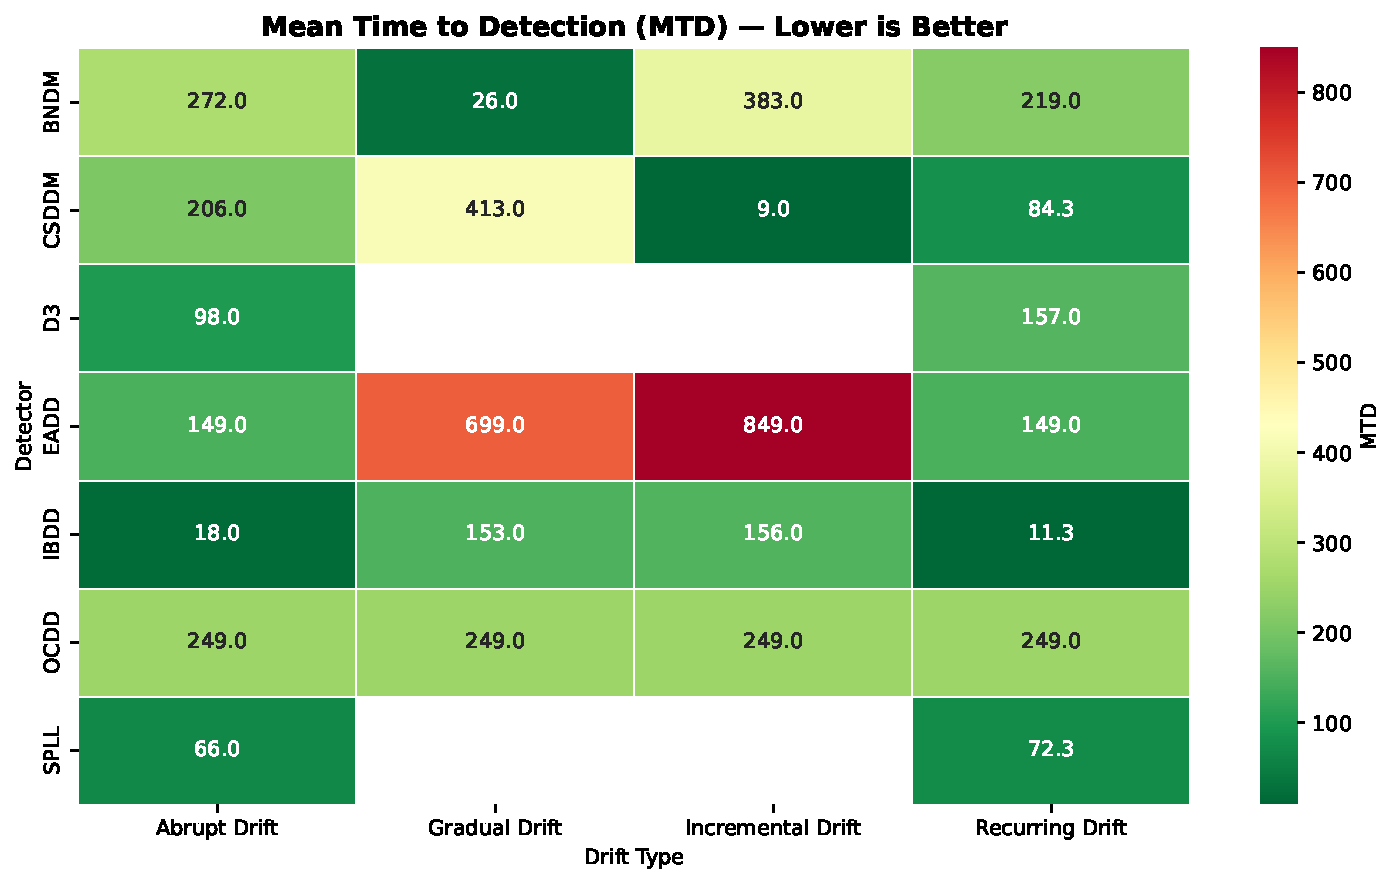
\includegraphics[width=\textwidth]{figures/heatmap_mtd.pdf}
    \end{minipage}
    \hfill
    \begin{minipage}{0.48\textwidth}
        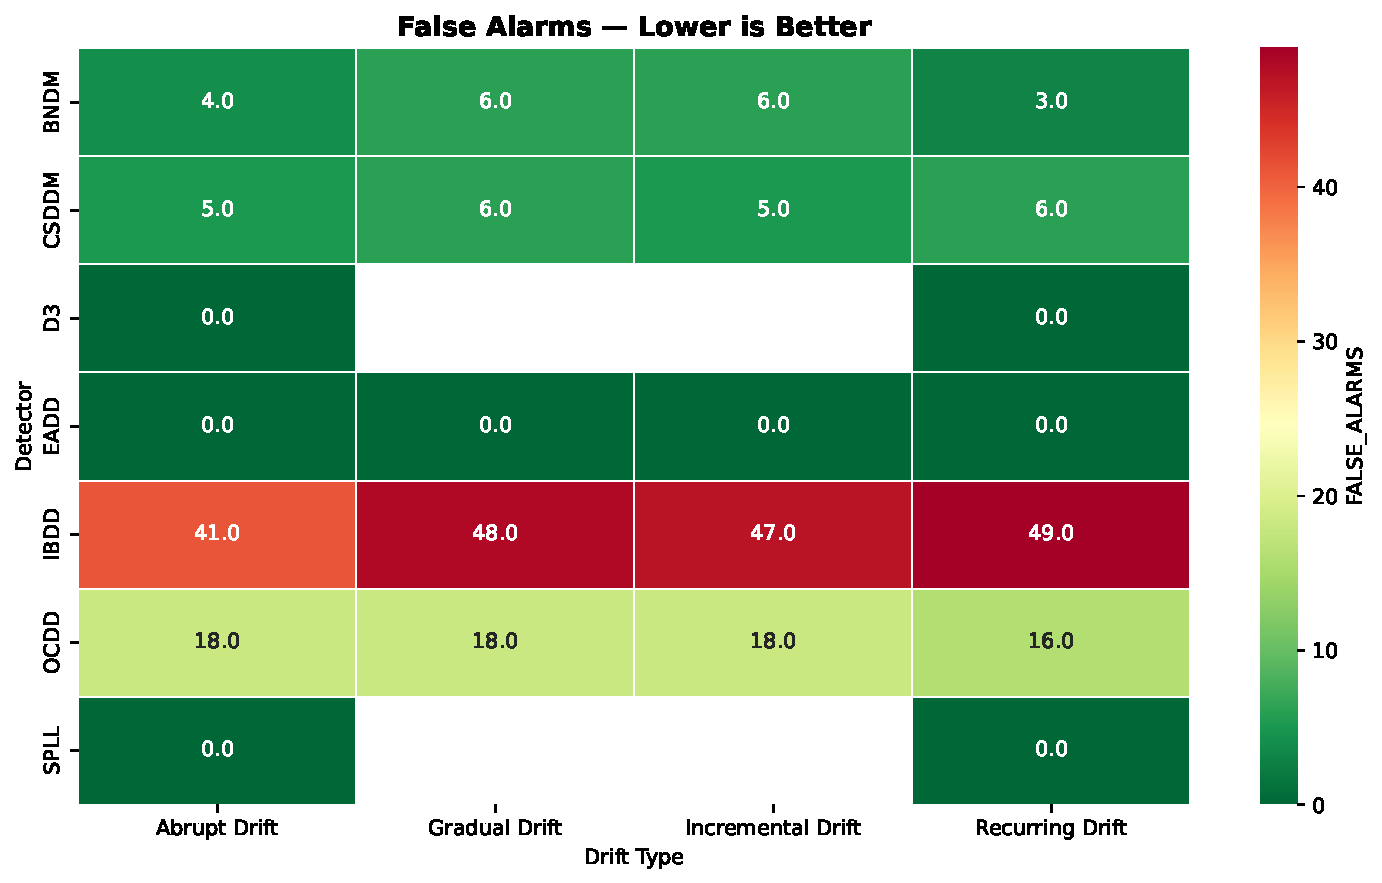
\includegraphics[width=\textwidth]{figures/heatmap_false_alarms.pdf}
    \end{minipage}
    \caption{Heatmaps of detection performance on synthetic drift. Left: Mean Time to Detection (lower is better; white cells indicate complete miss). Right: False Alarm count (lower is better).}
    \label{fig:heatmap-synthetic}
\end{figure}

Figure~\ref{fig:bell-curves-synthetic} shows the feature distribution bell curves before and after drift injection, visualizing the distributional shift that each detector must detect.

\begin{figure}[!htbp]
    \centering
    \begin{minipage}{0.48\textwidth}
        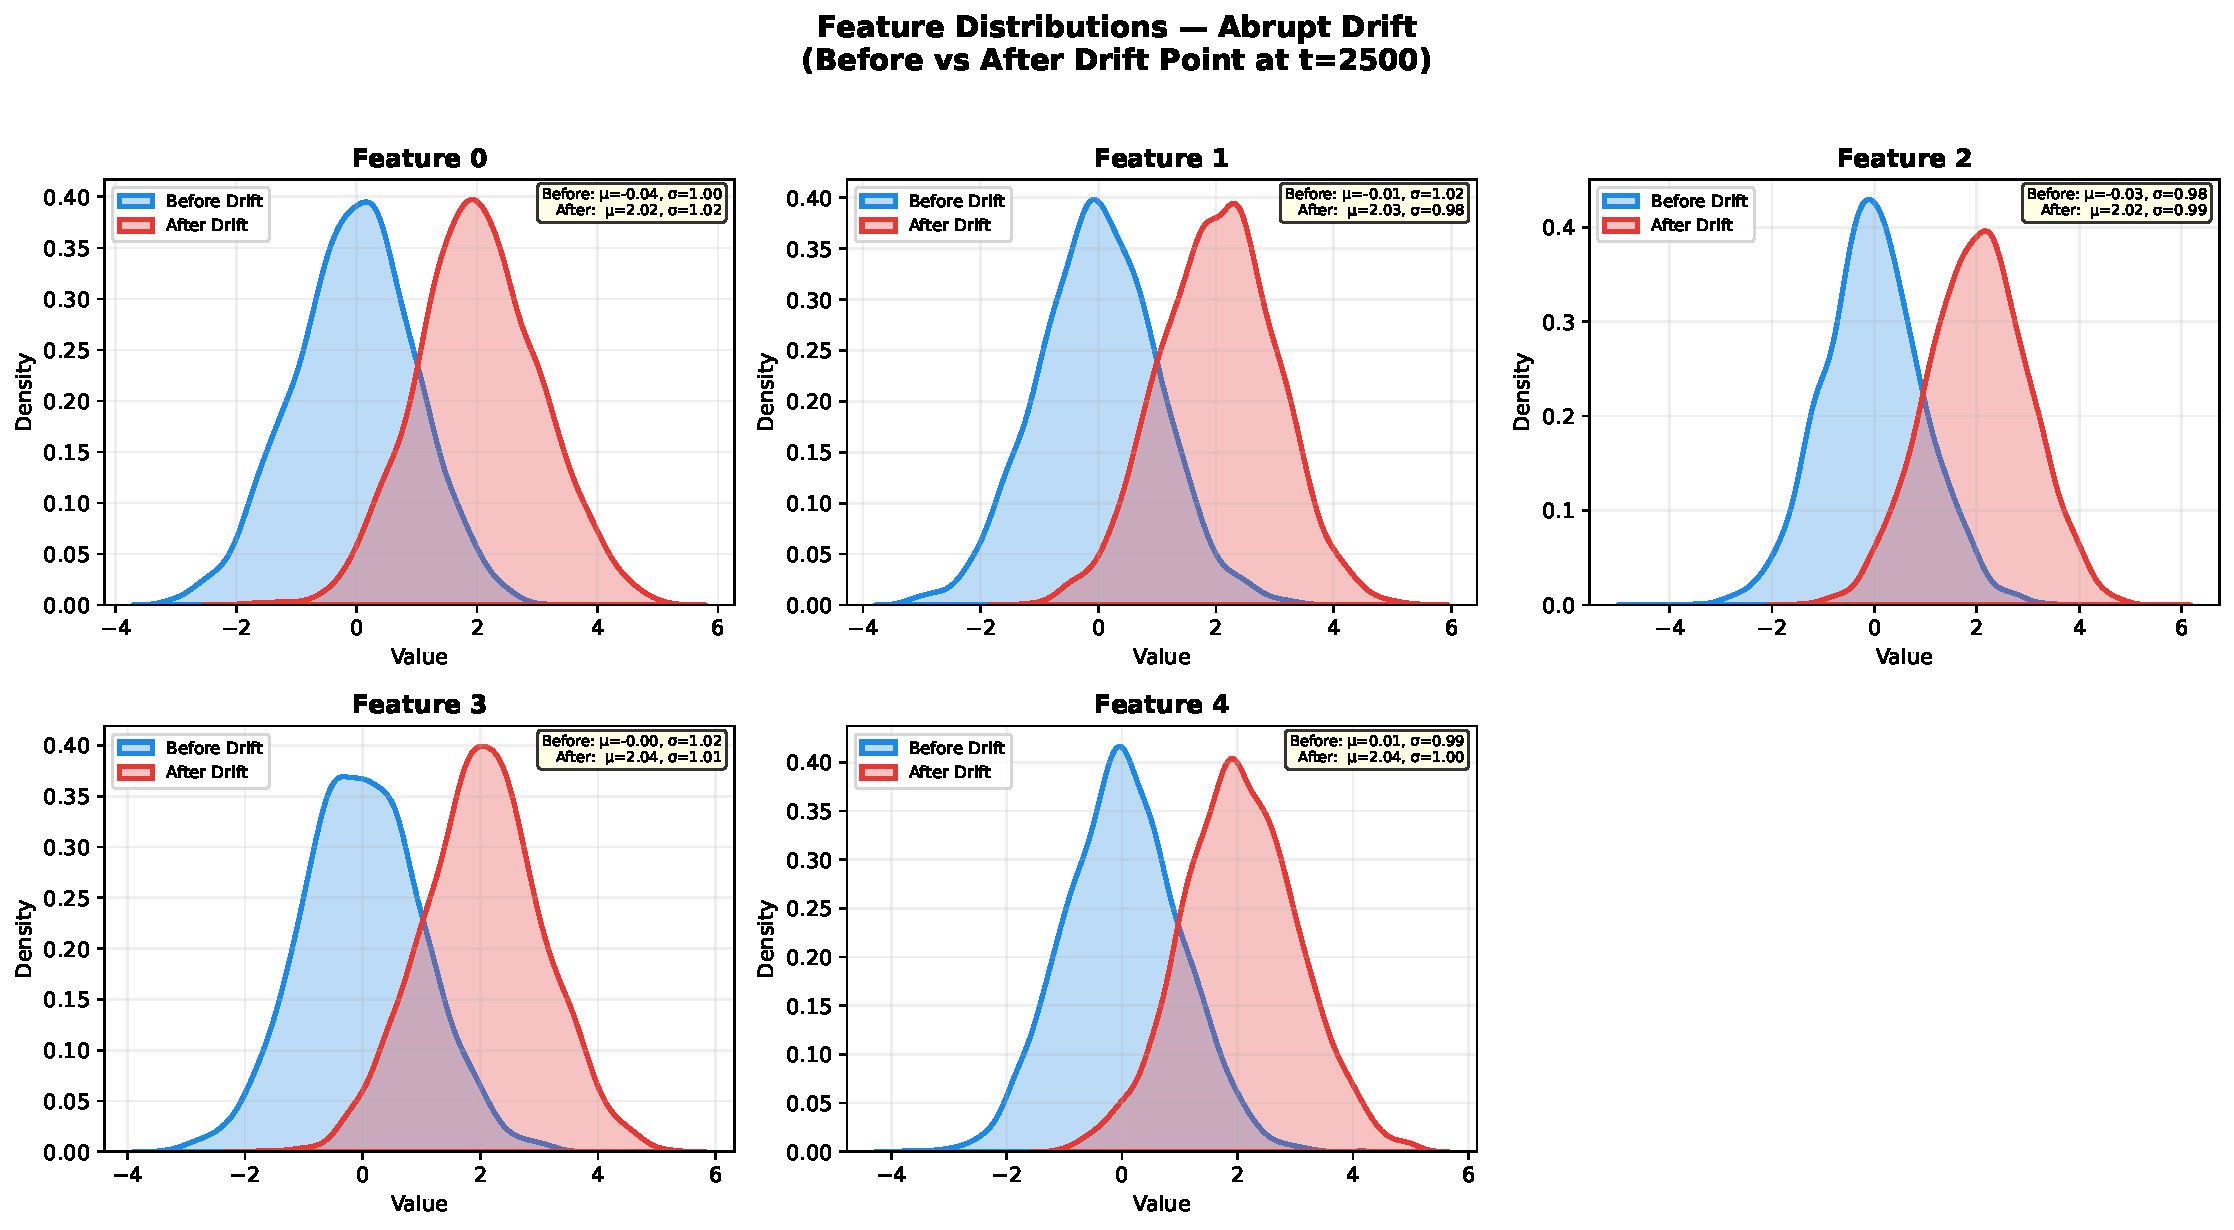
\includegraphics[width=\textwidth]{figures/bell_curves_abrupt_drift.pdf}
    \end{minipage}
    \hfill
    \begin{minipage}{0.48\textwidth}
        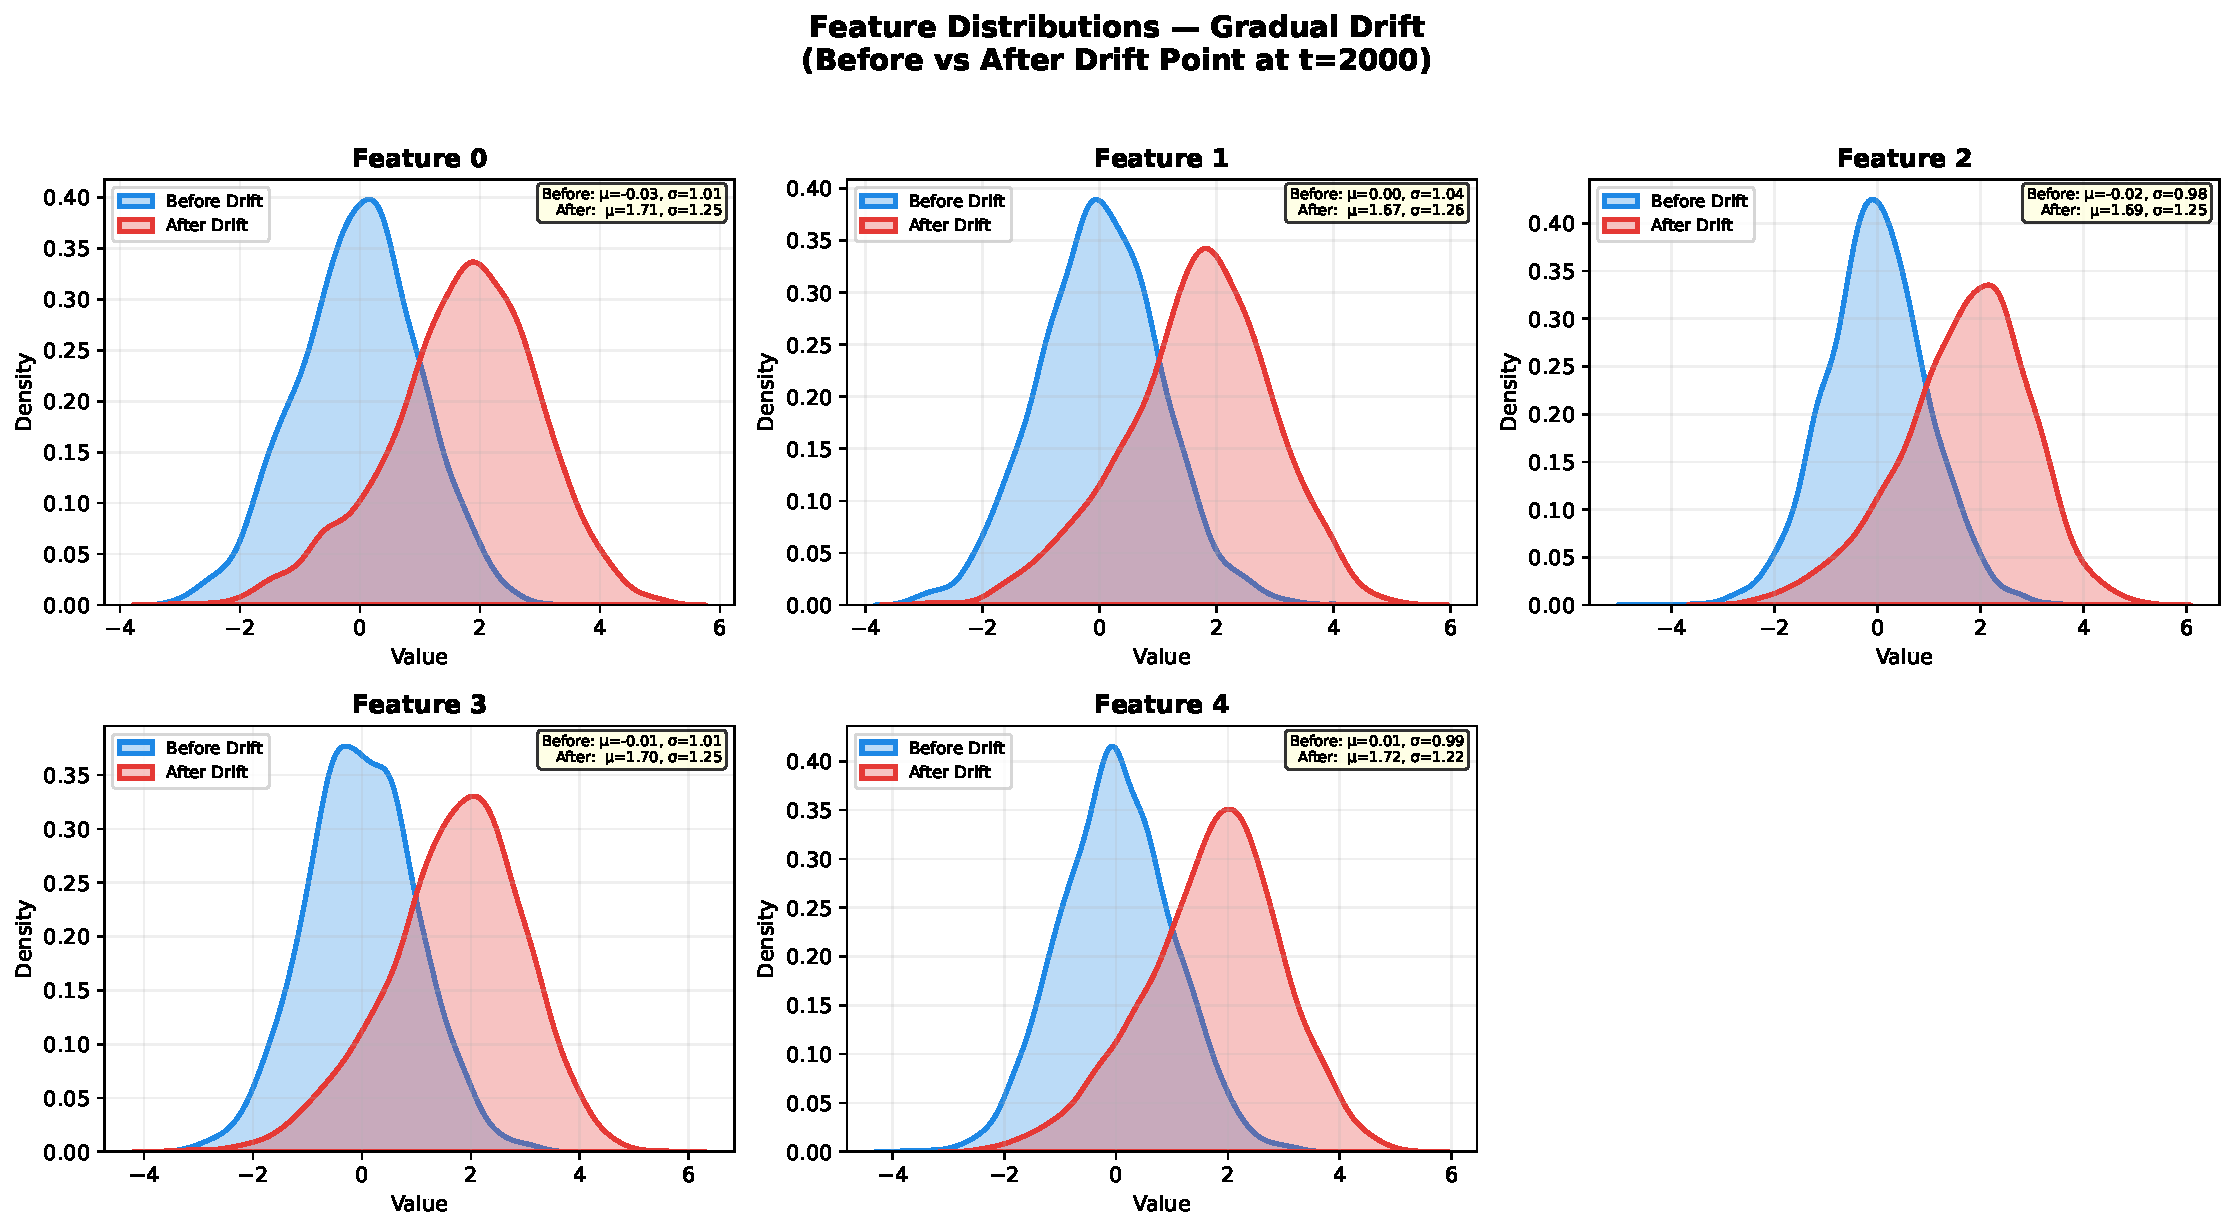
\includegraphics[width=\textwidth]{figures/bell_curves_gradual_drift.pdf}
    \end{minipage}
    \caption{Bell curves showing feature distributions before (blue) and after (red) drift injection. Left: Abrupt drift with clear separation. Right: Gradual drift with overlapping distributions---the subtle shift that D3, SPLL, and UDetect all failed to detect.}
    \label{fig:bell-curves-synthetic}
\end{figure}

Figure~\ref{fig:timeseries-synthetic} shows the multi-detector time-series comparison, plotting each detector's AUC or detection score over time alongside the true drift point.

\begin{figure}[!htbp]
    \centering
    \begin{minipage}{0.48\textwidth}
        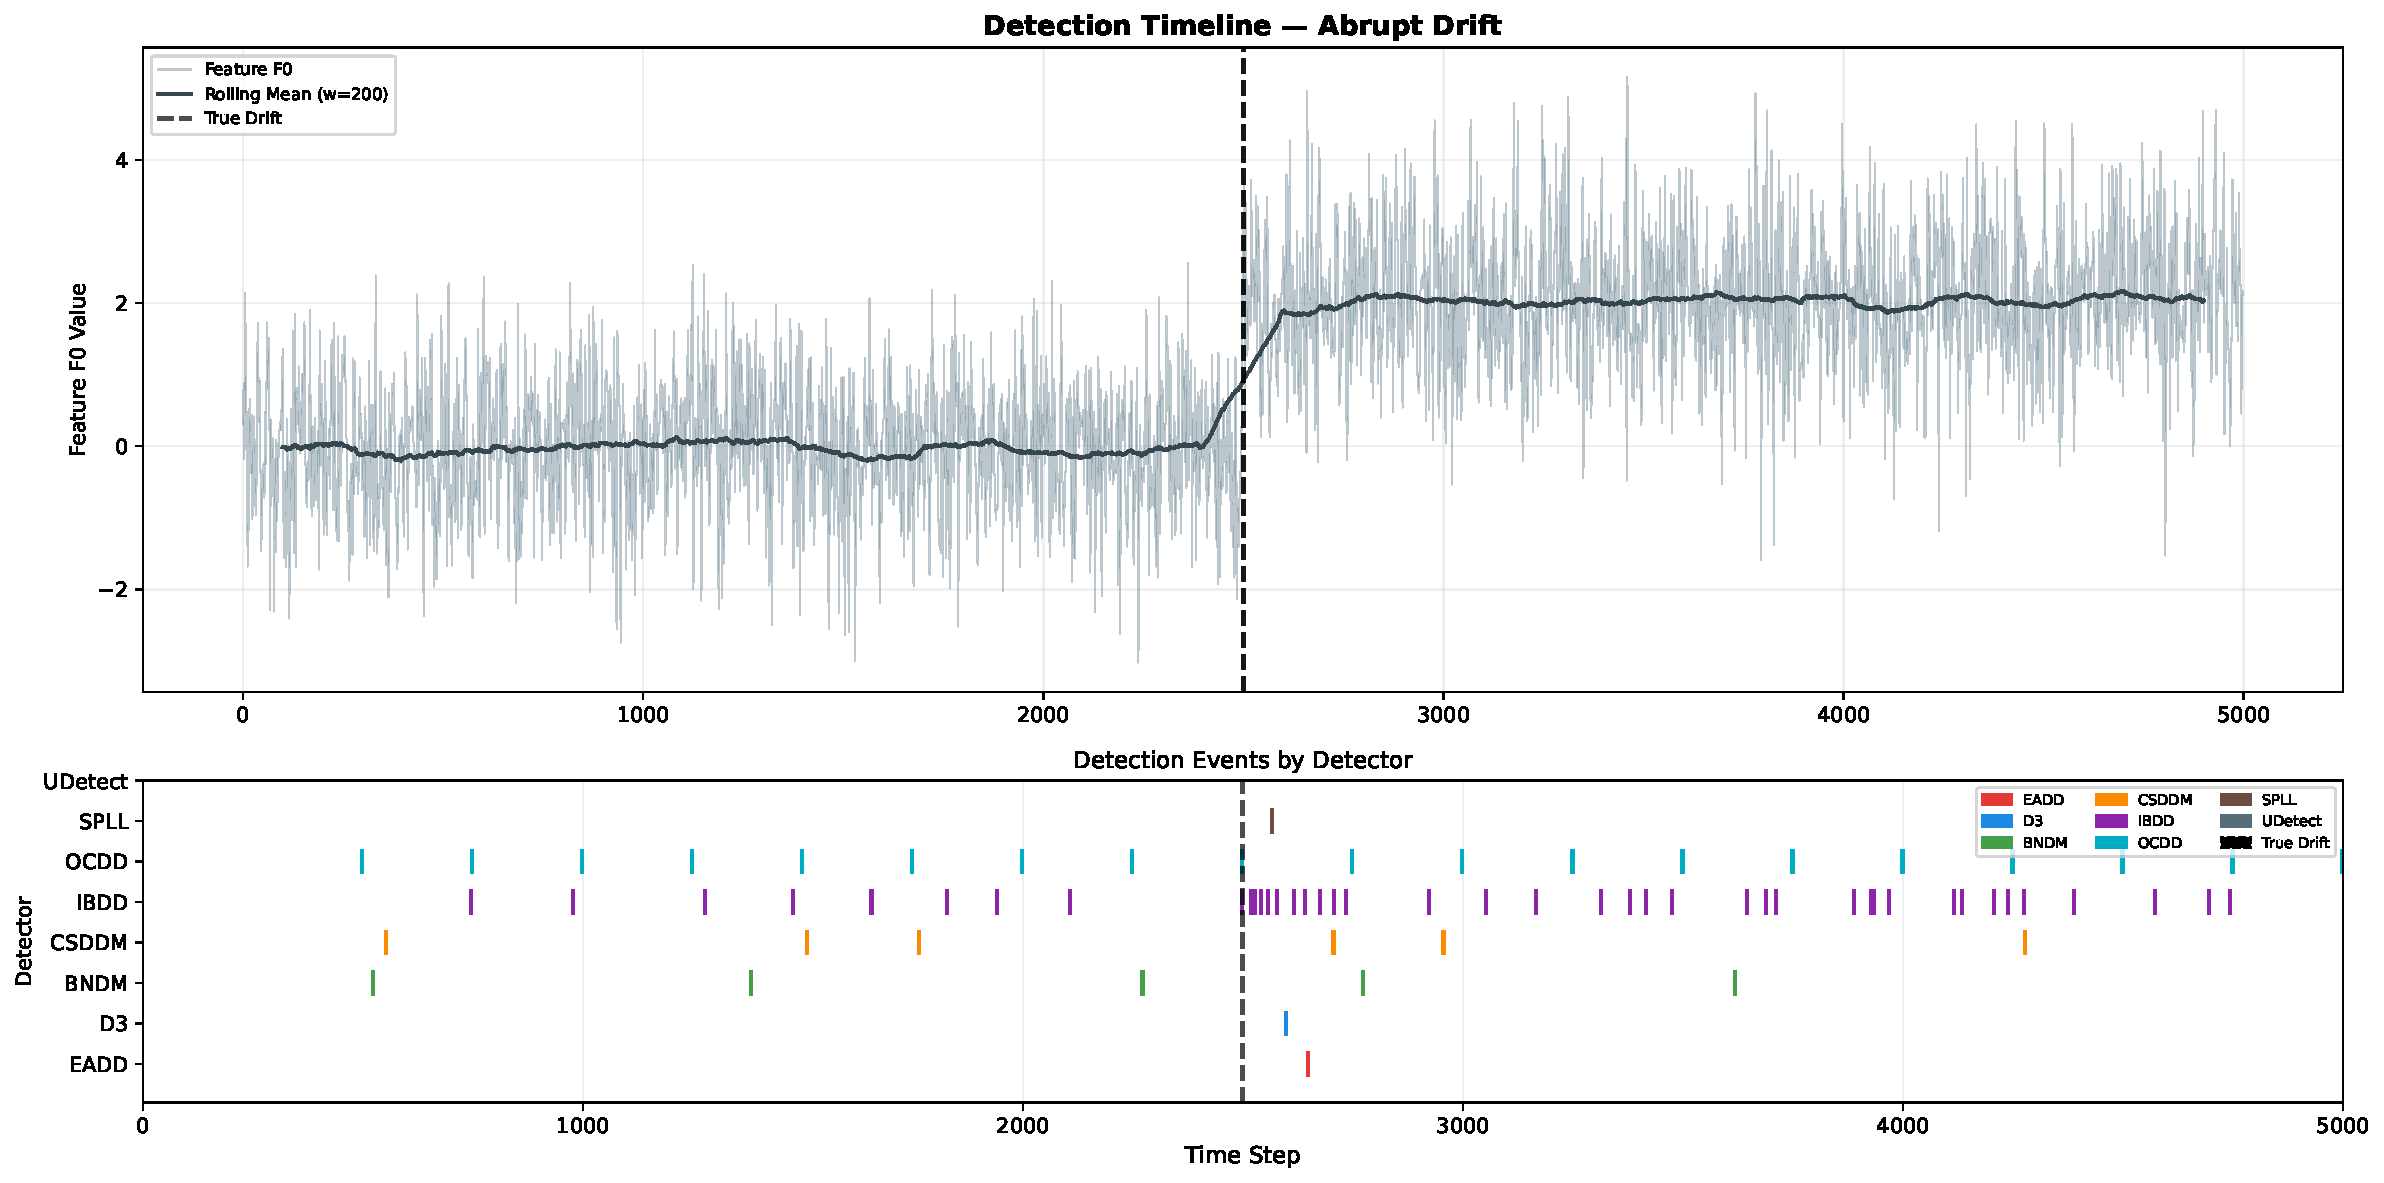
\includegraphics[width=\textwidth]{figures/timeseries_abrupt_drift.pdf}
    \end{minipage}
    \hfill
    \begin{minipage}{0.48\textwidth}
        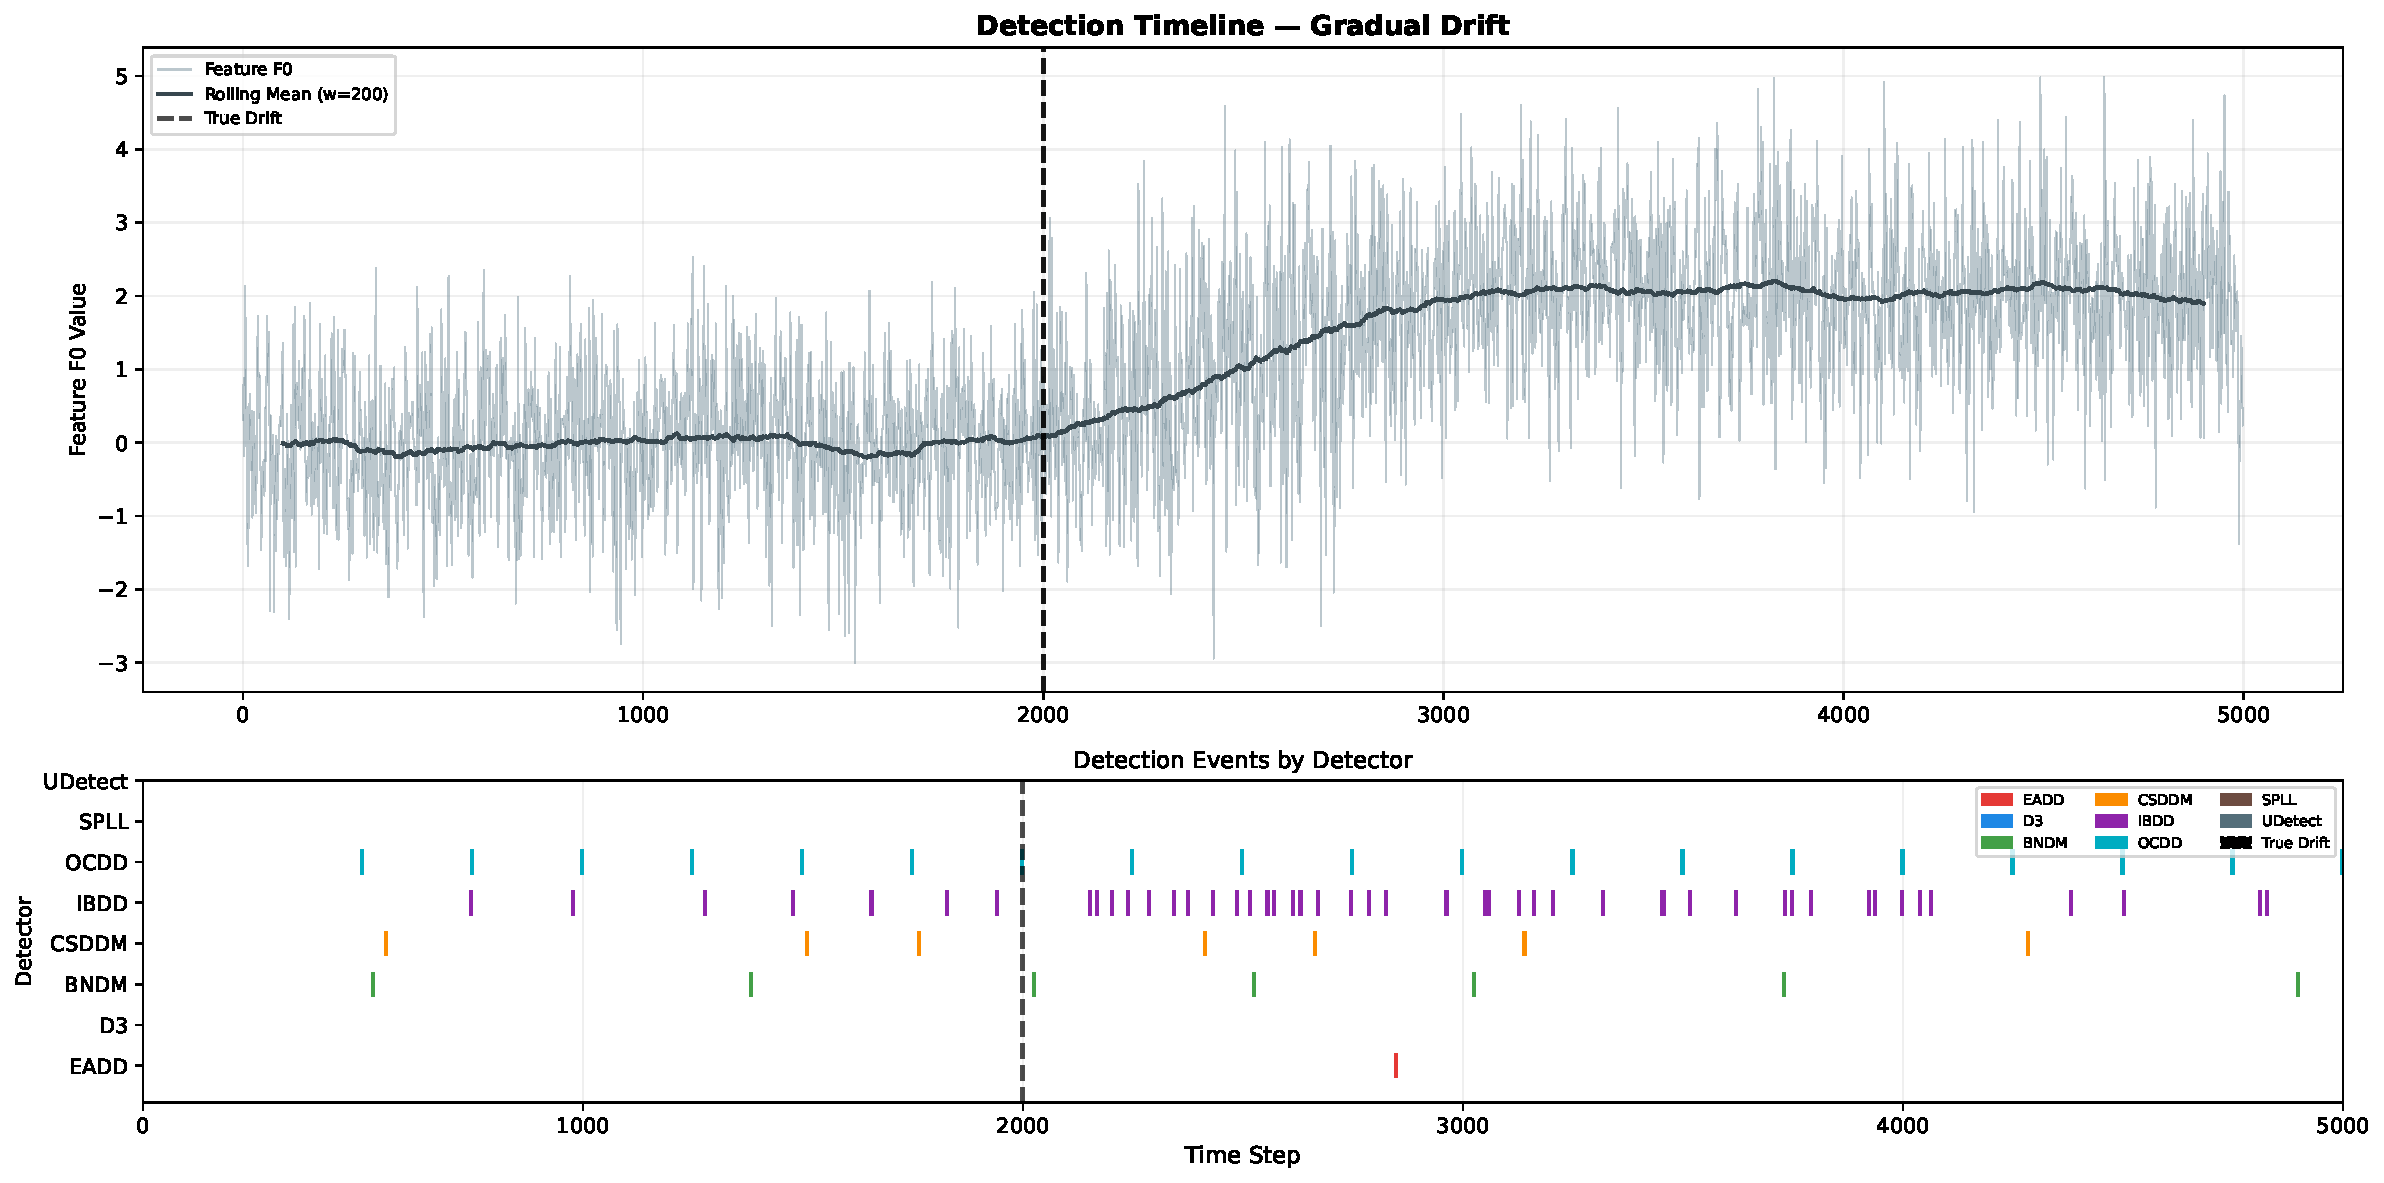
\includegraphics[width=\textwidth]{figures/timeseries_gradual_drift.pdf}
    \end{minipage}
    \caption{Time-series comparison of all eight detectors. Left: Abrupt drift---most detectors respond near the true drift point (dashed line). Right: Gradual drift---only EADD, BNDM, CSDDM, IBDD, and OCDD detect the shift; D3, SPLL, and UDetect remain silent.}
    \label{fig:timeseries-synthetic}
\end{figure}

\textbf{Key Findings:}
The multi-detector comparison reveals three distinct detector categories:

\begin{enumerate}
    \item \textbf{Complete Coverage with Low False Alarms:} EADD is the \textit{only} detector that detected all four drift types (MDR = 0) while maintaining near-zero false alarms (0--1 across all types). BNDM, CSDDM, and OCDD also detected all four types but produced 3--18 false alarms per type.
    
    \item \textbf{Complete Failures:} Three detectors failed on multiple drift types. D3 and SPLL both missed gradual and incremental drift entirely (MDR = 1.0), while UDetect failed on all four types.
    
    \item \textbf{Speed--Precision Trade-off:} IBDD achieved the fastest detection (MTD of 11--18 samples) but at an extreme cost of 41--49 false alarms per drift type---rendering it impractical for production monitoring where each false alarm triggers unnecessary investigation or retraining.
\end{enumerate}

Critically, EADD is the only detector that combines complete drift coverage (4/4 types detected, 0\% MDR) with false alarm discipline ($\leq 1$ false alarm across all experiments). The permutation test provides the statistical rigor that separates EADD from other complete-coverage detectors like BNDM (3--6 false alarms per type) and CSDDM (5--6 per type).

\section{Experiment 2: Multi-Detector Real-World Benchmark}

\textbf{Objective:} Evaluate all eight detectors on real-world data streams from the \citet{Lukats2025} benchmark where drift patterns are unknown, complex, and multi-dimensional.

\textbf{Procedure:}
Eleven real-world datasets from the \citet{Lukats2025} benchmark were processed in streaming fashion. All eight detectors were applied with their default configurations. For datasets with known ground-truth drift points (InsectsAbrupt, InsectsGradual, SineClusters, WaveformDrift2), standard detection metrics (MTD, MDR) were computed. For datasets without ground truth, the number of detections was recorded.

A per-detector timeout of 120 seconds was applied, as BNDM's BaggedNearestDelta computation exceeded practical limits on high-dimensional (33-feature) datasets.

\textbf{Results:}

Table~\ref{tab:exp2-results} presents the results on datasets with known drift points.

\begin{table}[!htbp]
\centering
\caption{Experiment 2: Multi-Detector Benchmark on Datasets with Known Drift Points. MTD = Mean Time to Detection; MDR = Missed Detection Rate. Bold indicates best MTD among detectors with MDR = 0. ``---'' indicates detector missed all drifts or timed out.}
\label{tab:exp2-results}
\begin{tabular}{l|cc|cc|cc|cc}
\hline
 & \multicolumn{2}{c|}{\textbf{InsectsAbrupt}} & \multicolumn{2}{c|}{\textbf{InsectsGradual}} & \multicolumn{2}{c|}{\textbf{SineClusters}} & \multicolumn{2}{c}{\textbf{WaveformDrift2}} \\
\textbf{Detector} & MTD & MDR & MTD & MDR & MTD & MDR & MTD & MDR \\
\hline
\textbf{EADD} & 173 & 0.0 & --- & 1.0 & 266 & 0.0 & \textbf{99} & 0.0 \\
D3 & 153 & 0.0 & --- & 1.0 & 219 & 0.0 & 179 & 0.0 \\
BNDM & --- & --- & --- & 1.0 & 499 & 0.0 & 60 & 0.0 \\
CSDDM & \textbf{44} & 0.0 & \textbf{143} & 0.0 & \textbf{35} & 0.0 & 359 & 0.0 \\
IBDD & 28 & 0.0 & 88 & 0.0 & 45 & 0.0 & \textbf{8} & 0.0 \\
OCDD & 254 & 0.5 & --- & 1.0 & 249 & 0.0 & 249 & 0.0 \\
SPLL & \textbf{25} & 0.0 & 39 & 0.0 & 249 & 0.0 & 22 & 0.0 \\
UDetect & --- & --- & --- & --- & 36 & 0.67 & 21 & 0.33 \\
\hline
\end{tabular}
\end{table}

Table~\ref{tab:exp2-nogt} summarizes detection activity on datasets without annotated ground-truth drift points.

\begin{table}[!htbp]
\centering
\caption{Experiment 2: Detection Counts on Datasets Without Ground Truth (lower is generally preferred, as excessive detections suggest false alarms). ``TO'' = timed out.}
\label{tab:exp2-nogt}
\begin{tabular}{lccccccc}
\hline
\textbf{Dataset} & \textbf{EADD} & \textbf{D3} & \textbf{BNDM} & \textbf{CSDDM} & \textbf{IBDD} & \textbf{OCDD} & \textbf{SPLL} \\
\hline
Electricity & 39 & 37 & 40 & 79 & 726 & 37 & 75 \\
IncrAbrupt & 1 & 0 & TO & 15 & 94 & 79 & 0 \\
Incremental & 1 & 0 & TO & 19 & 63 & 79 & 1 \\
Reoccurring & 2 & 2 & TO & 21 & 107 & 79 & 1 \\
NOAAWeather & 12 & 29 & 36 & 70 & 485 & 71 & 2 \\
OutdoorObjects & 6 & 1 & 8 & 15 & 34 & 15 & 14 \\
Powersupply & 6 & 11 & 16 & 58 & 163 & 79 & 9 \\
\hline
\textbf{Total} & \textbf{67} & \textbf{80} & --- & \textbf{277} & \textbf{1{,}672} & \textbf{439} & \textbf{102} \\
\hline
\end{tabular}
\end{table}

Figure~\ref{fig:heatmap-realworld} presents heatmaps summarizing detection performance across all detector--dataset combinations on the real-world benchmark.

\begin{figure}[!htbp]
    \centering
    \begin{minipage}{0.48\textwidth}
        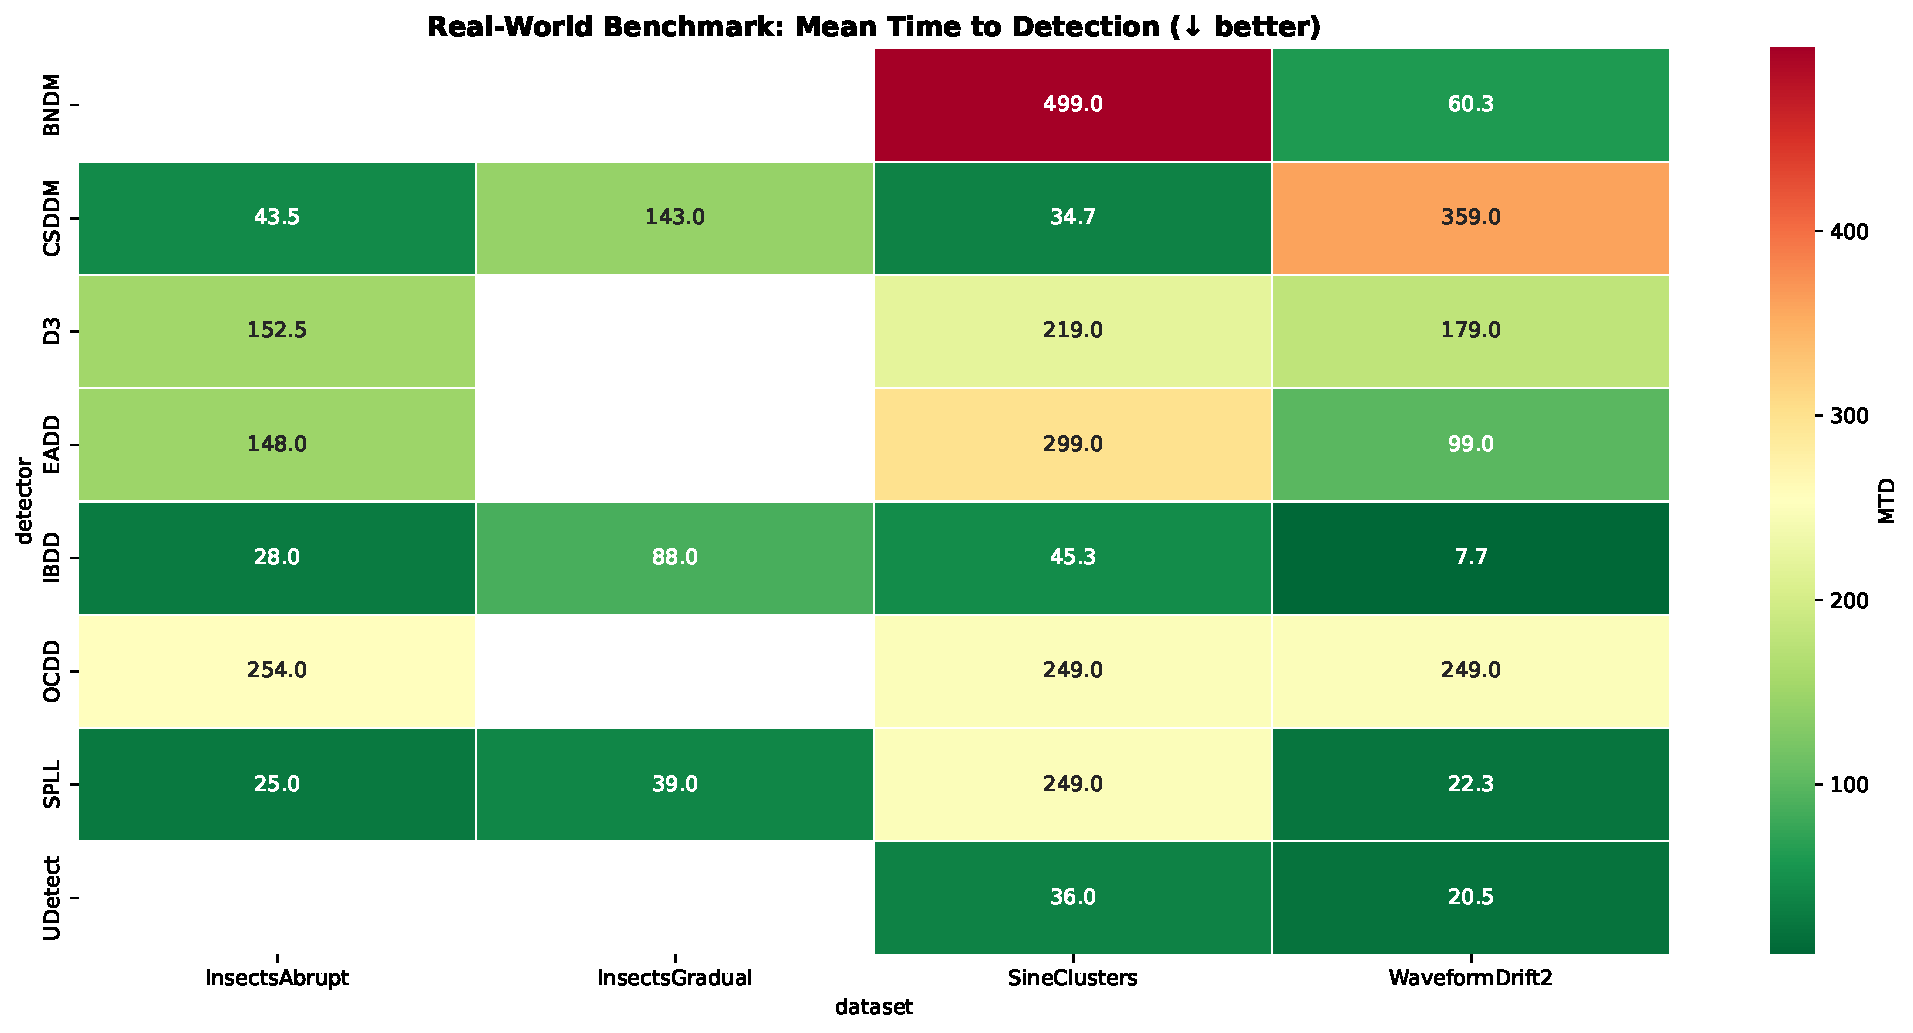
\includegraphics[width=\textwidth]{figures/heatmap_realworld_mtd.pdf}
    \end{minipage}
    \hfill
    \begin{minipage}{0.48\textwidth}
        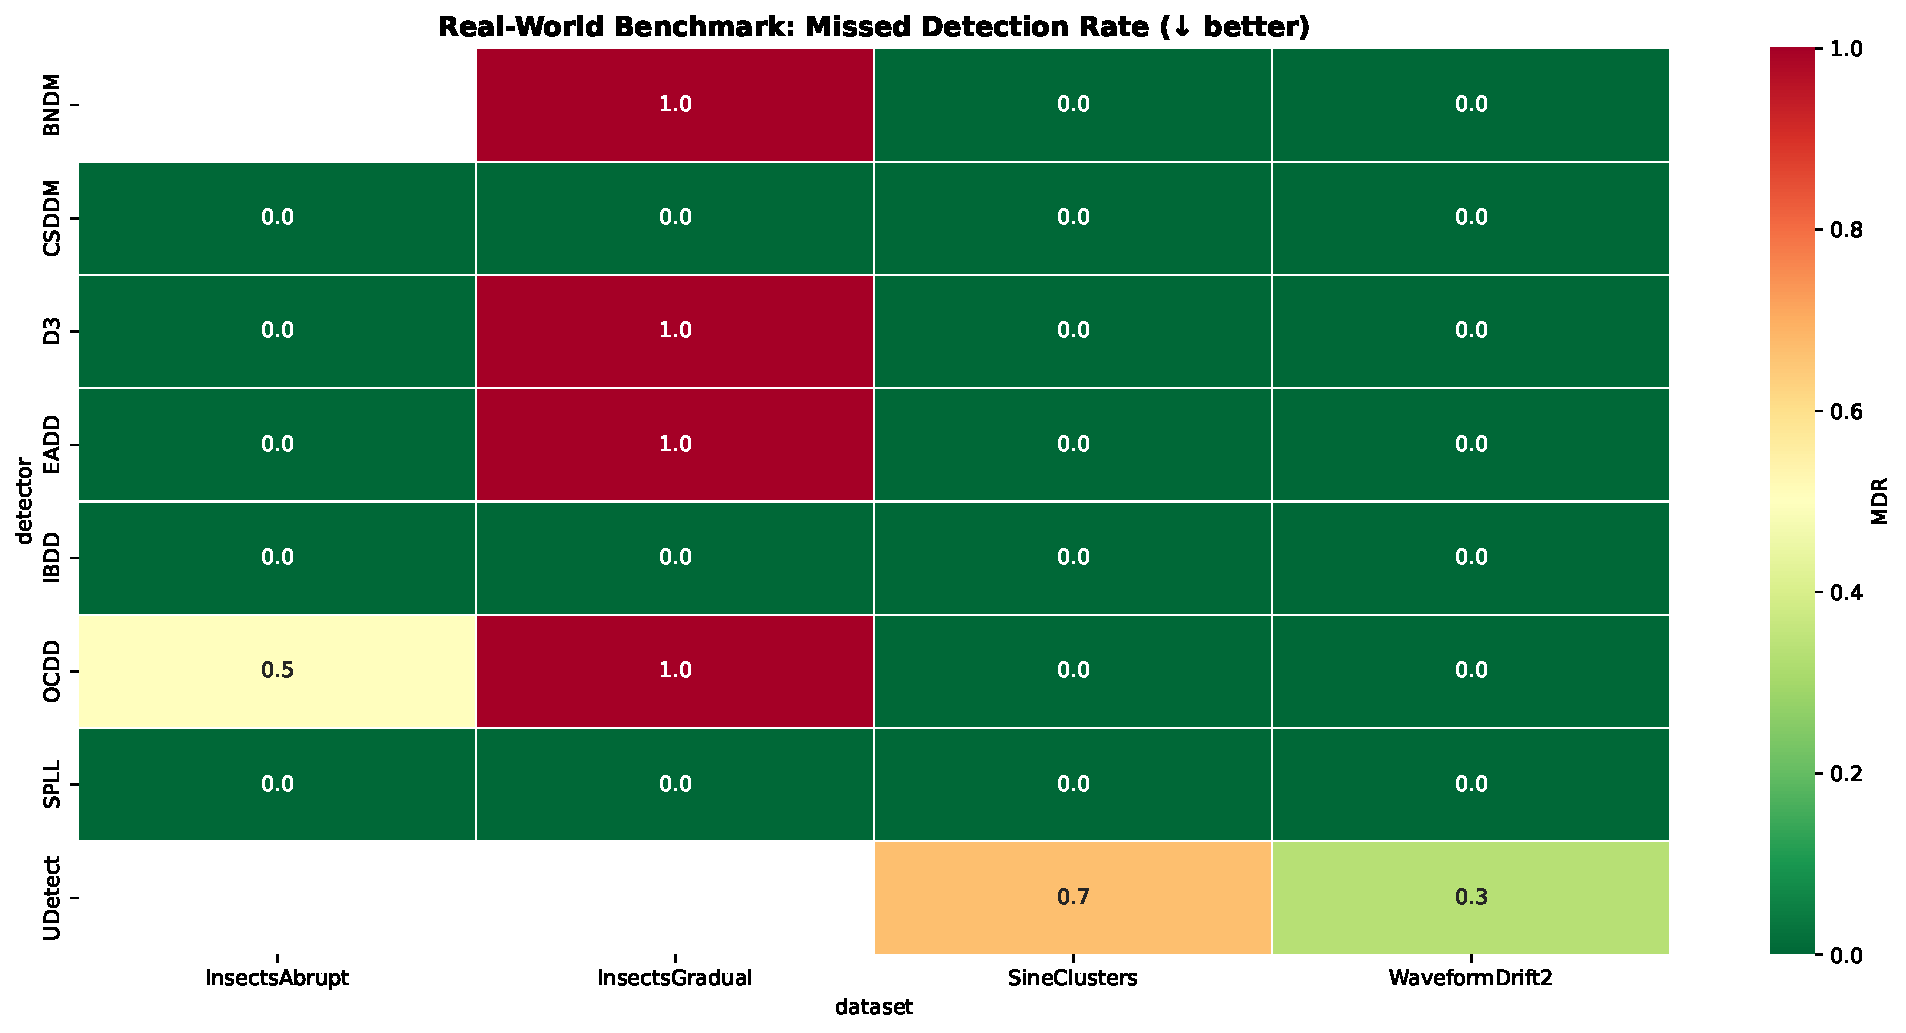
\includegraphics[width=\textwidth]{figures/heatmap_realworld_mdr.pdf}
    \end{minipage}
    \caption{Heatmaps of real-world benchmark performance. Left: Mean Time to Detection (lower is better; white cells indicate missed drifts or timeout). Right: Missed Detection Rate (0.0 is perfect).}
    \label{fig:heatmap-realworld}
\end{figure}

Figure~\ref{fig:timeseries-realworld} shows time-series visualizations of detection behavior on two representative real-world datasets.

\begin{figure}[!htbp]
    \centering
    \begin{minipage}{0.48\textwidth}
        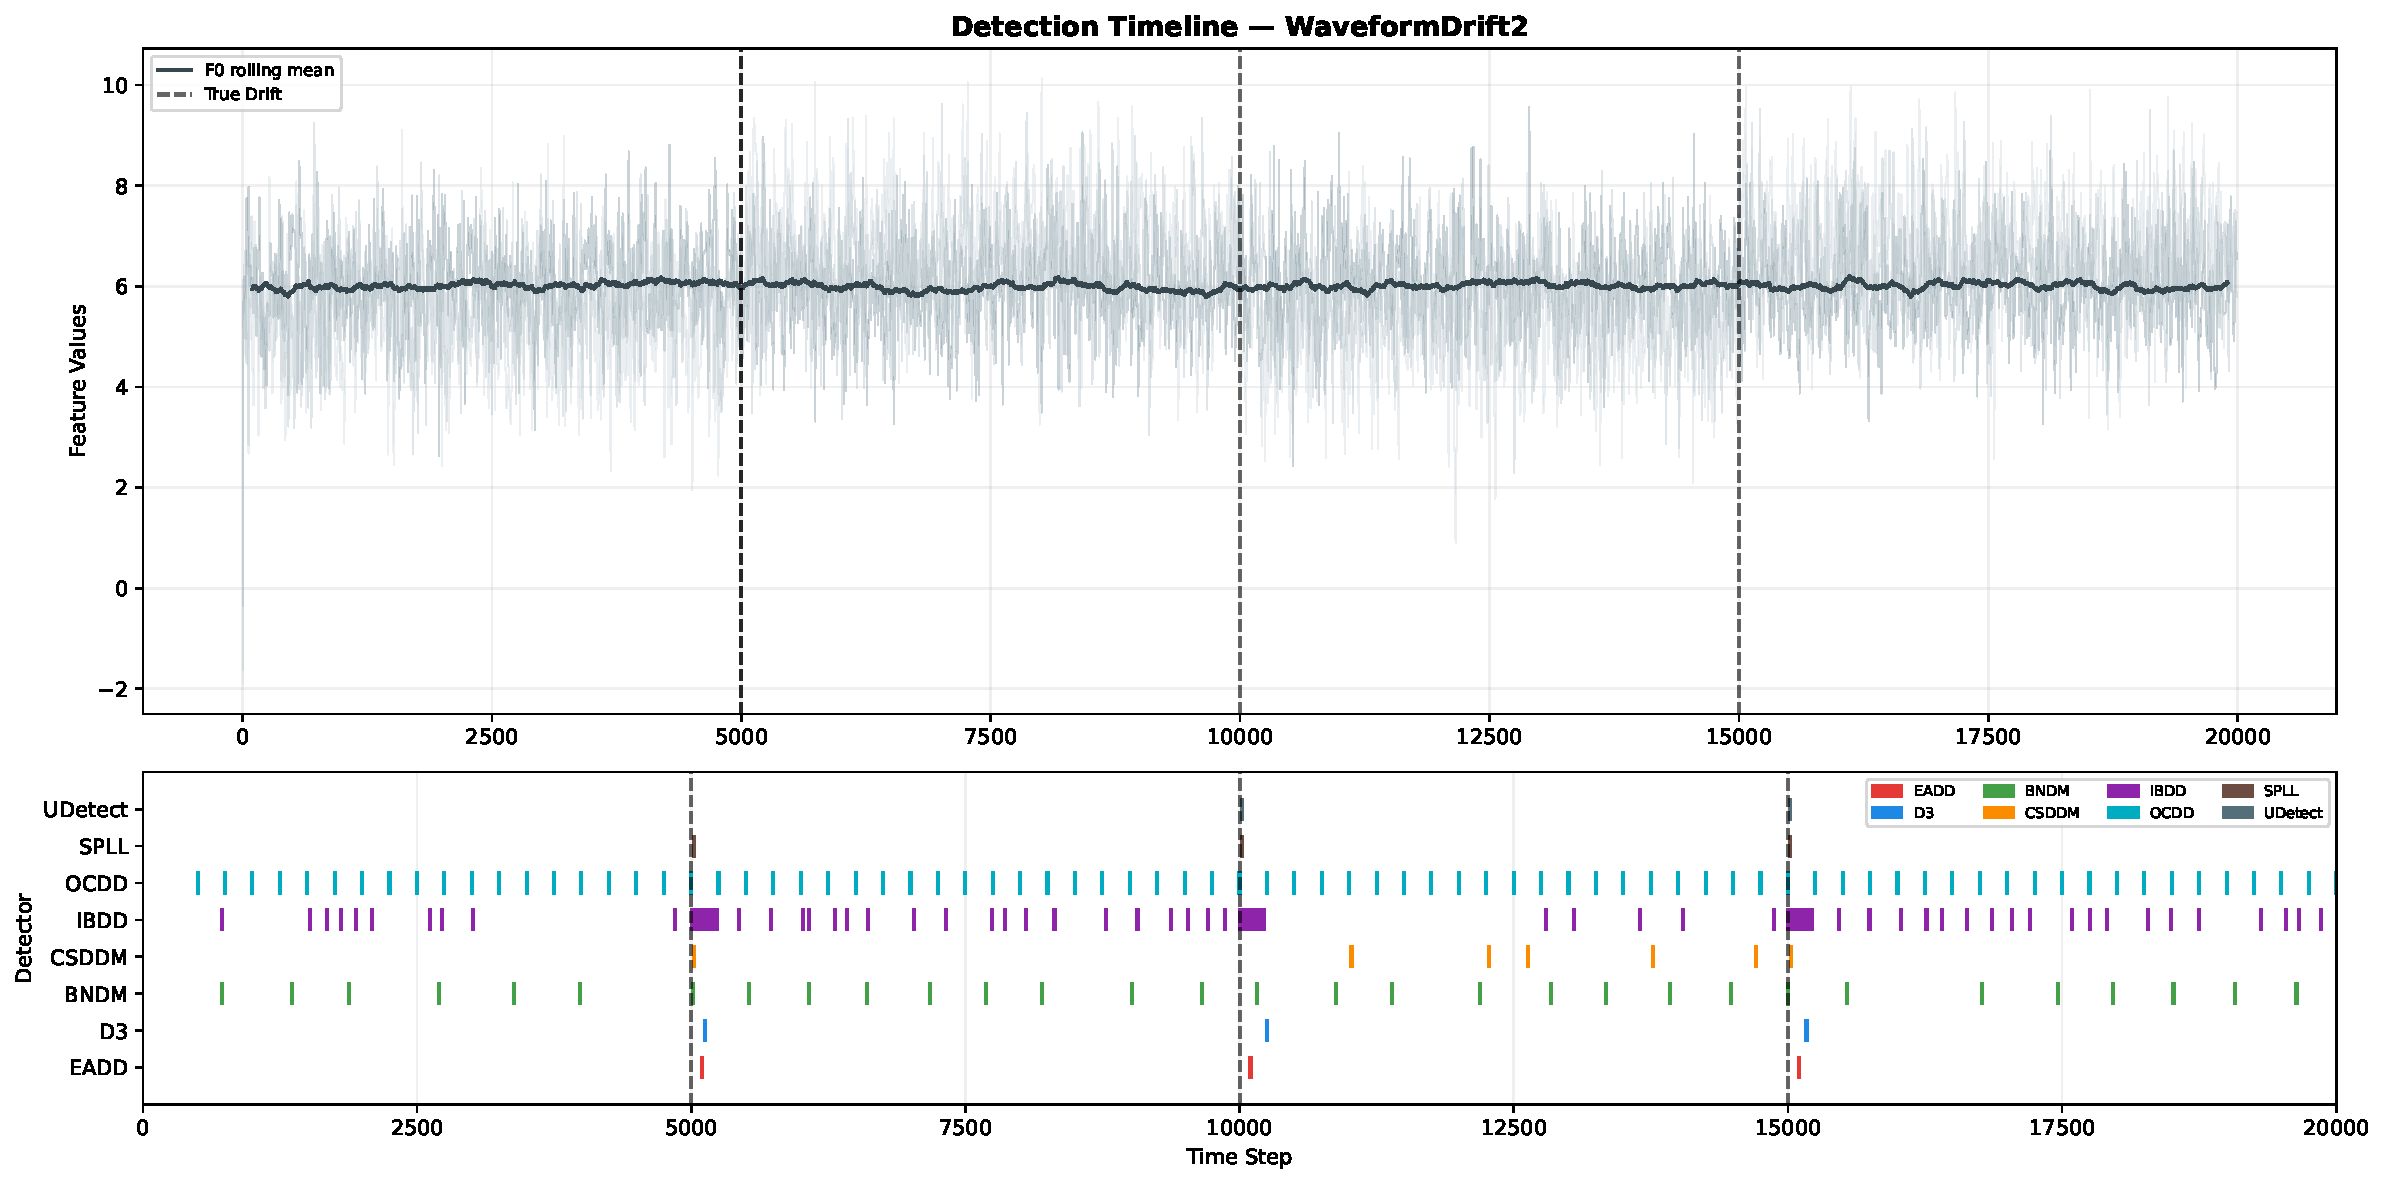
\includegraphics[width=\textwidth]{figures/timeseries_realworld_waveformdrift2.pdf}
    \end{minipage}
    \hfill
    \begin{minipage}{0.48\textwidth}
        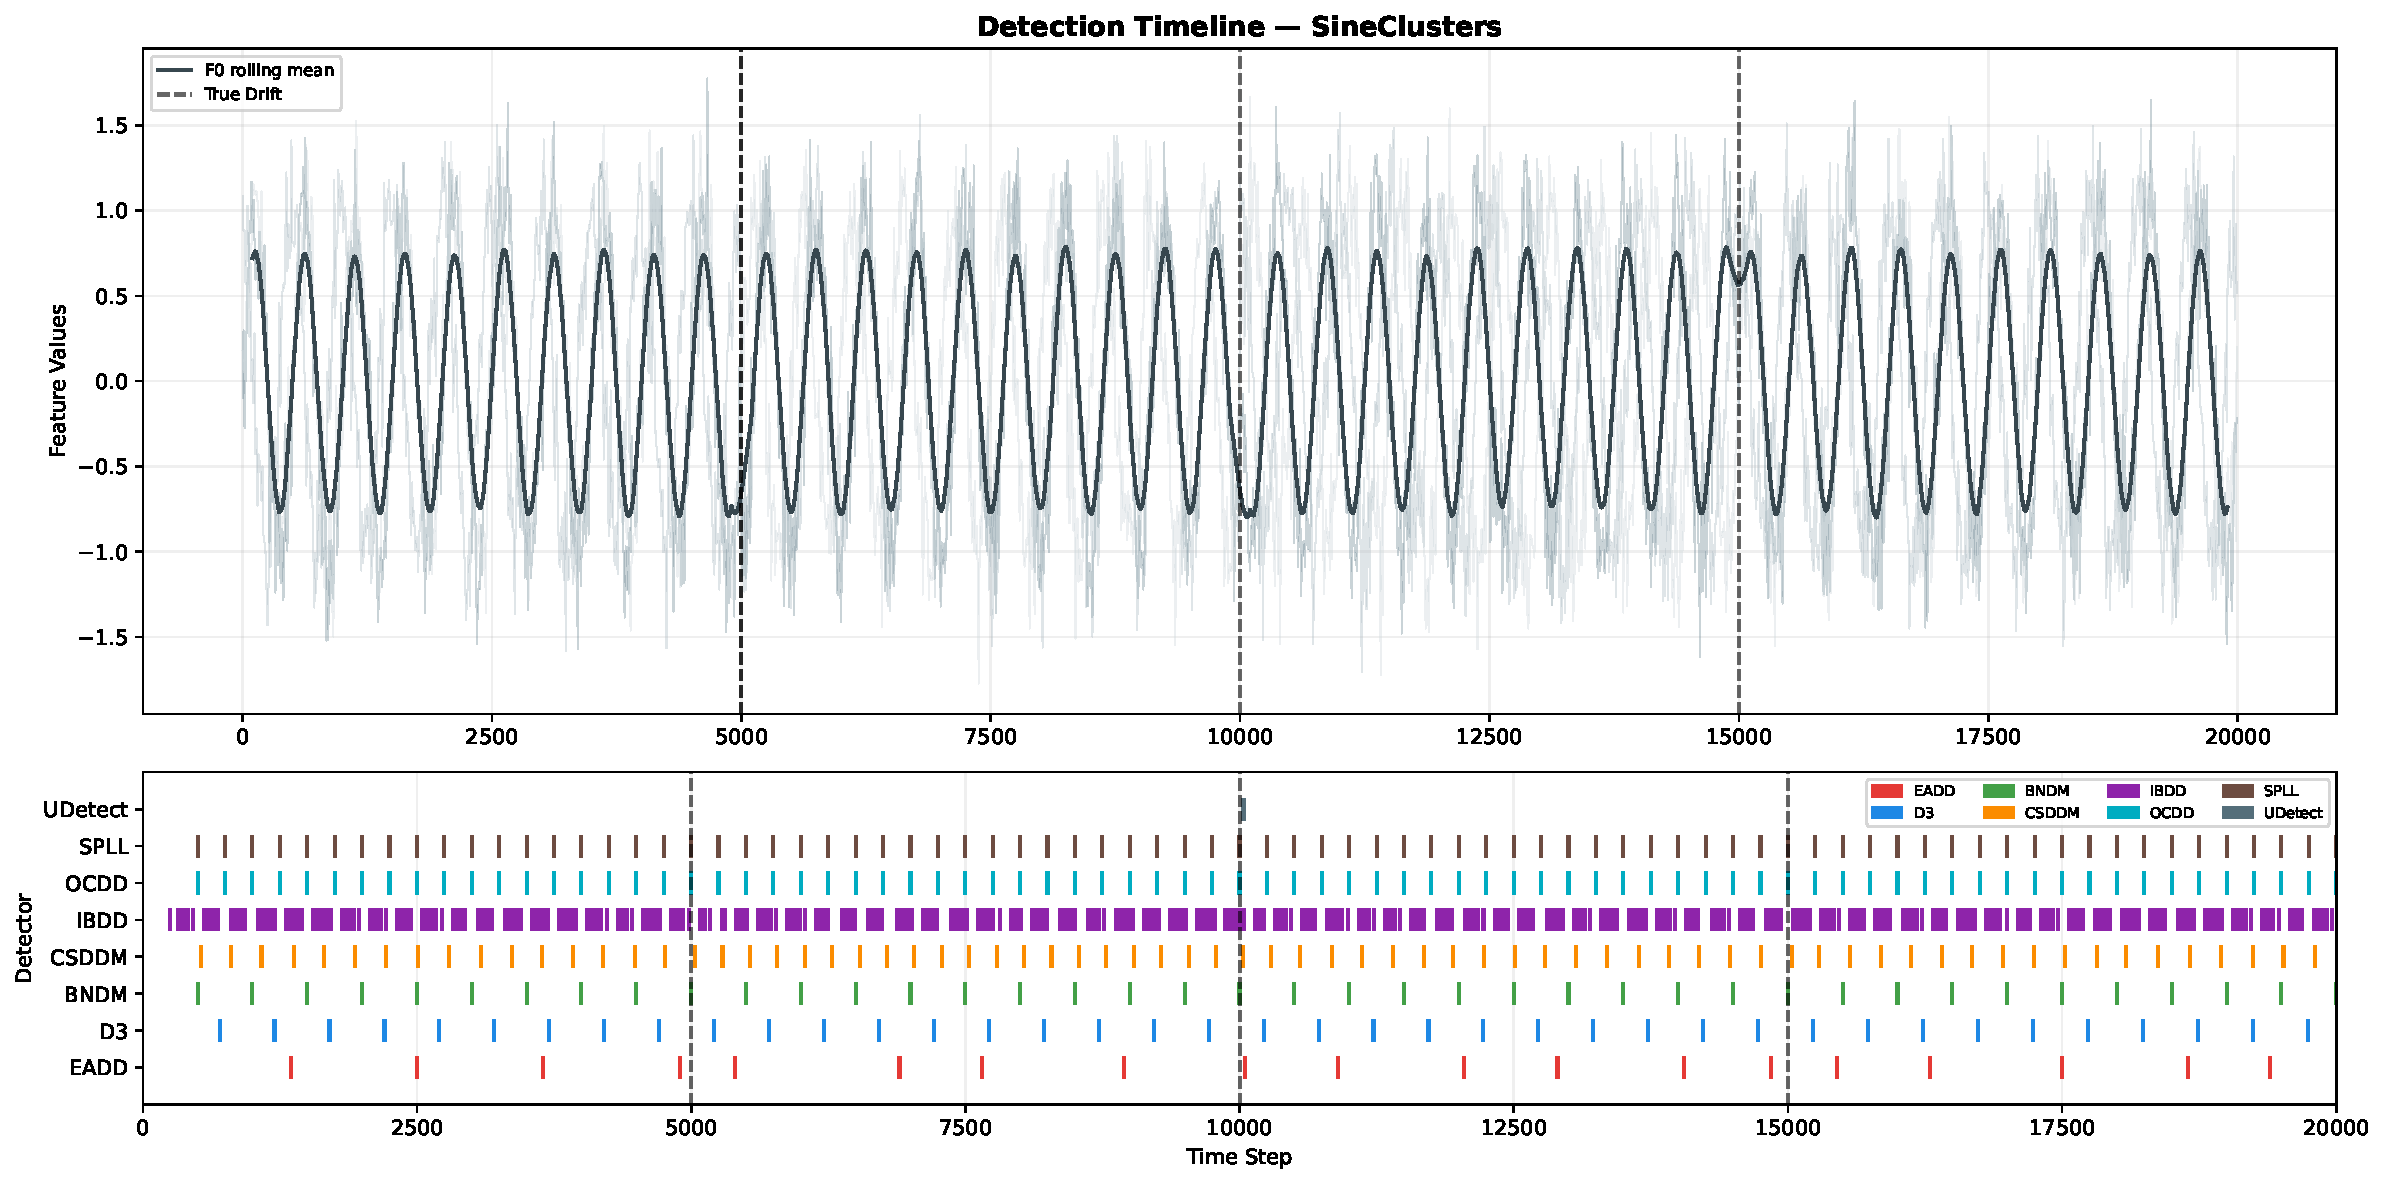
\includegraphics[width=\textwidth]{figures/timeseries_realworld_sineclusters.pdf}
    \end{minipage}
    \caption{Time-series comparison on real-world datasets. Left: WaveformDrift2---EADD (MTD=99) responds faster than D3 (MTD=179) with zero false alarms. Right: SineClusters---all detectors except UDetect detect at least some drift points; IBDD detects rapidly but with 612 excess detections.}
    \label{fig:timeseries-realworld}
\end{figure}

Figure~\ref{fig:bell-curves-realworld} shows the bell curve distributions for representative real-world datasets, illustrating the distributional complexity that detectors must handle.

\begin{figure}[!htbp]
    \centering
    \begin{minipage}{0.48\textwidth}
        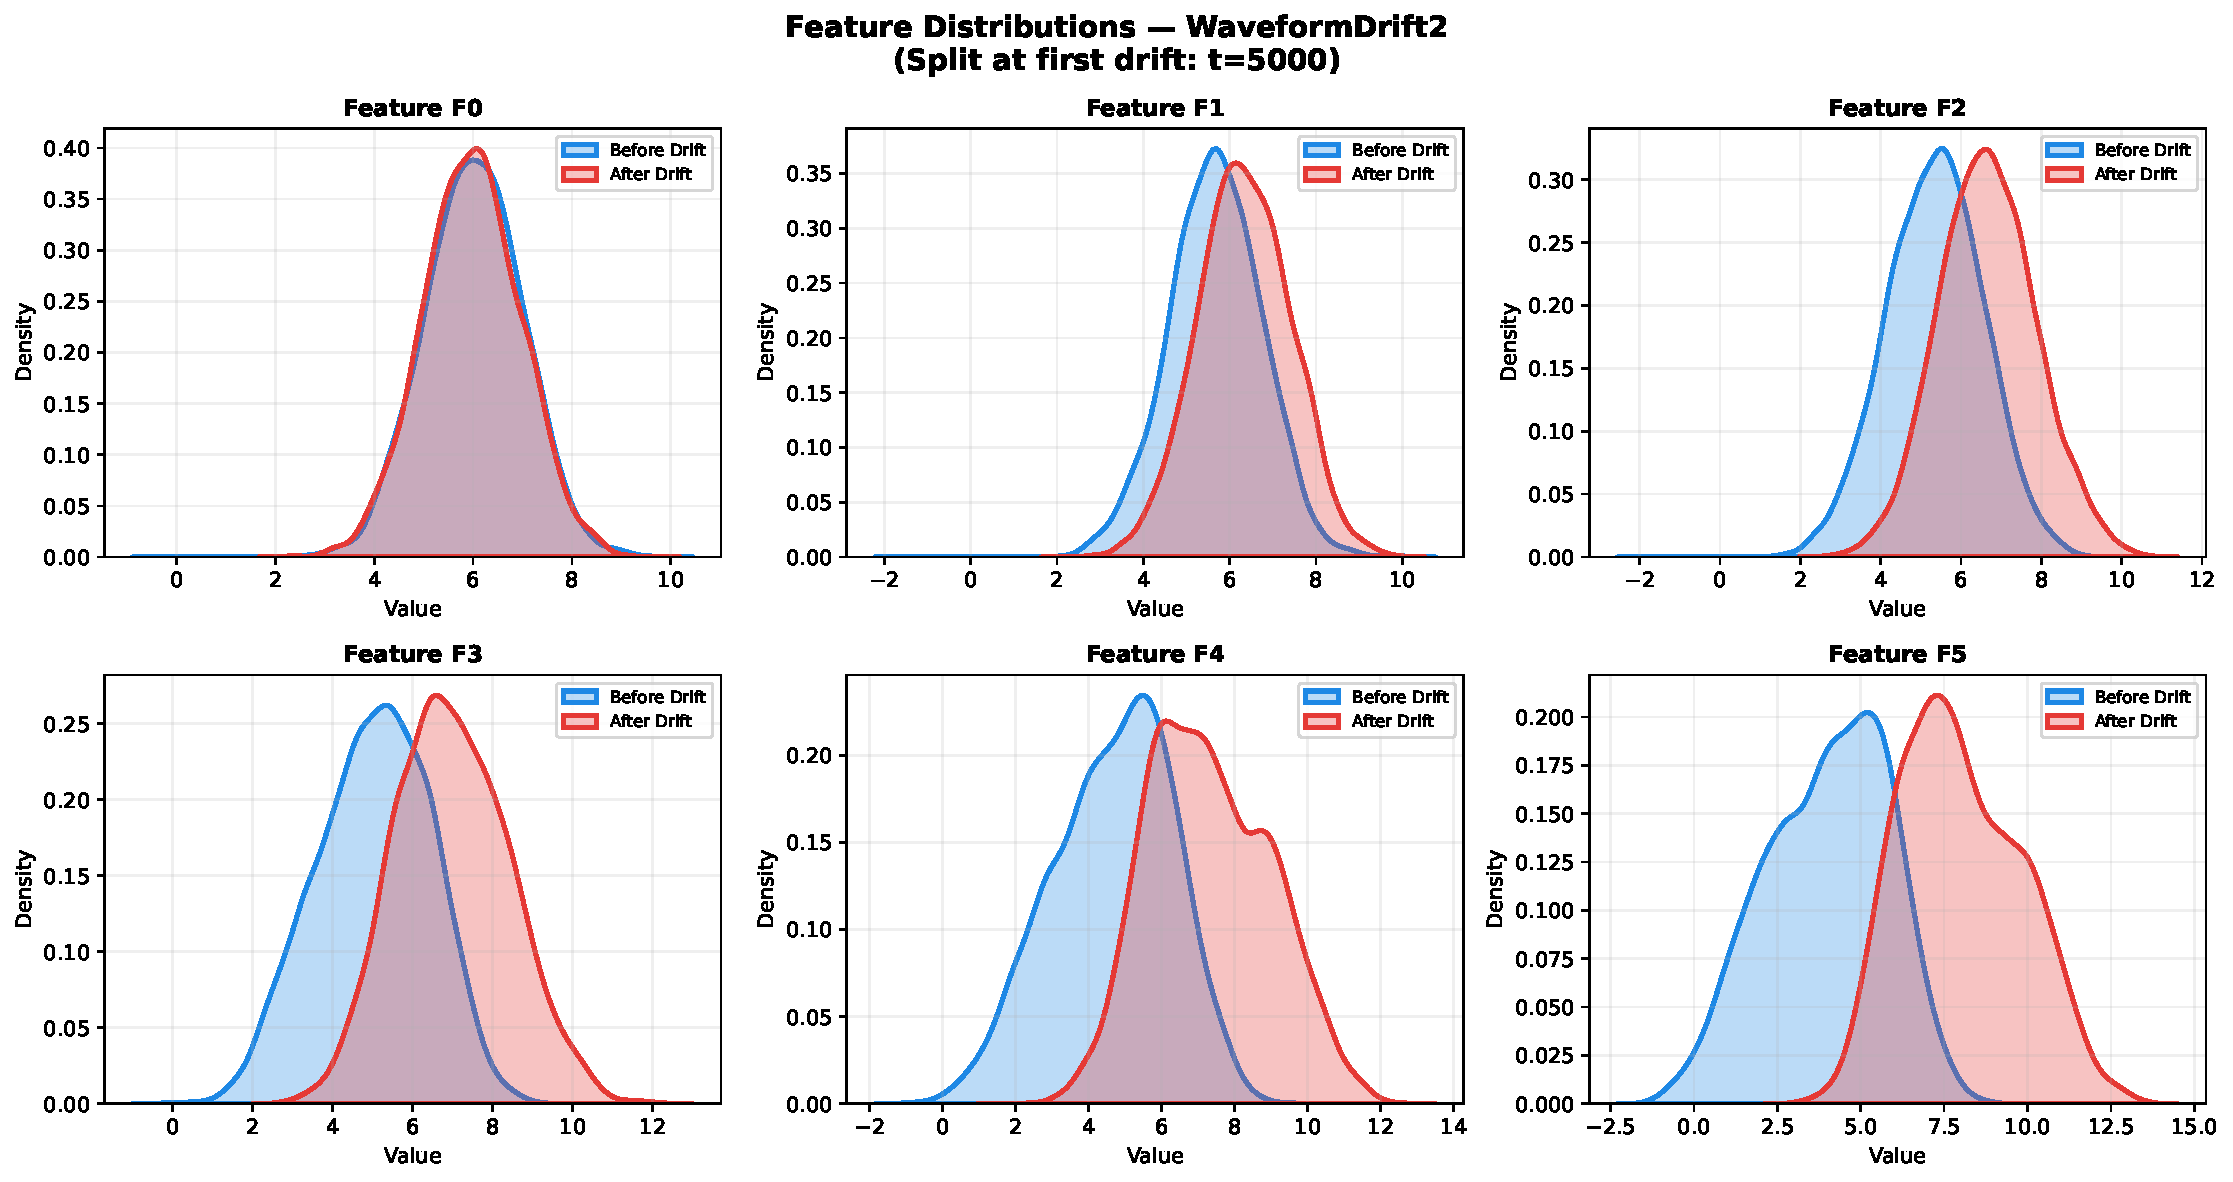
\includegraphics[width=\textwidth]{figures/bell_curves_realworld_waveformdrift2.pdf}
    \end{minipage}
    \hfill
    \begin{minipage}{0.48\textwidth}
        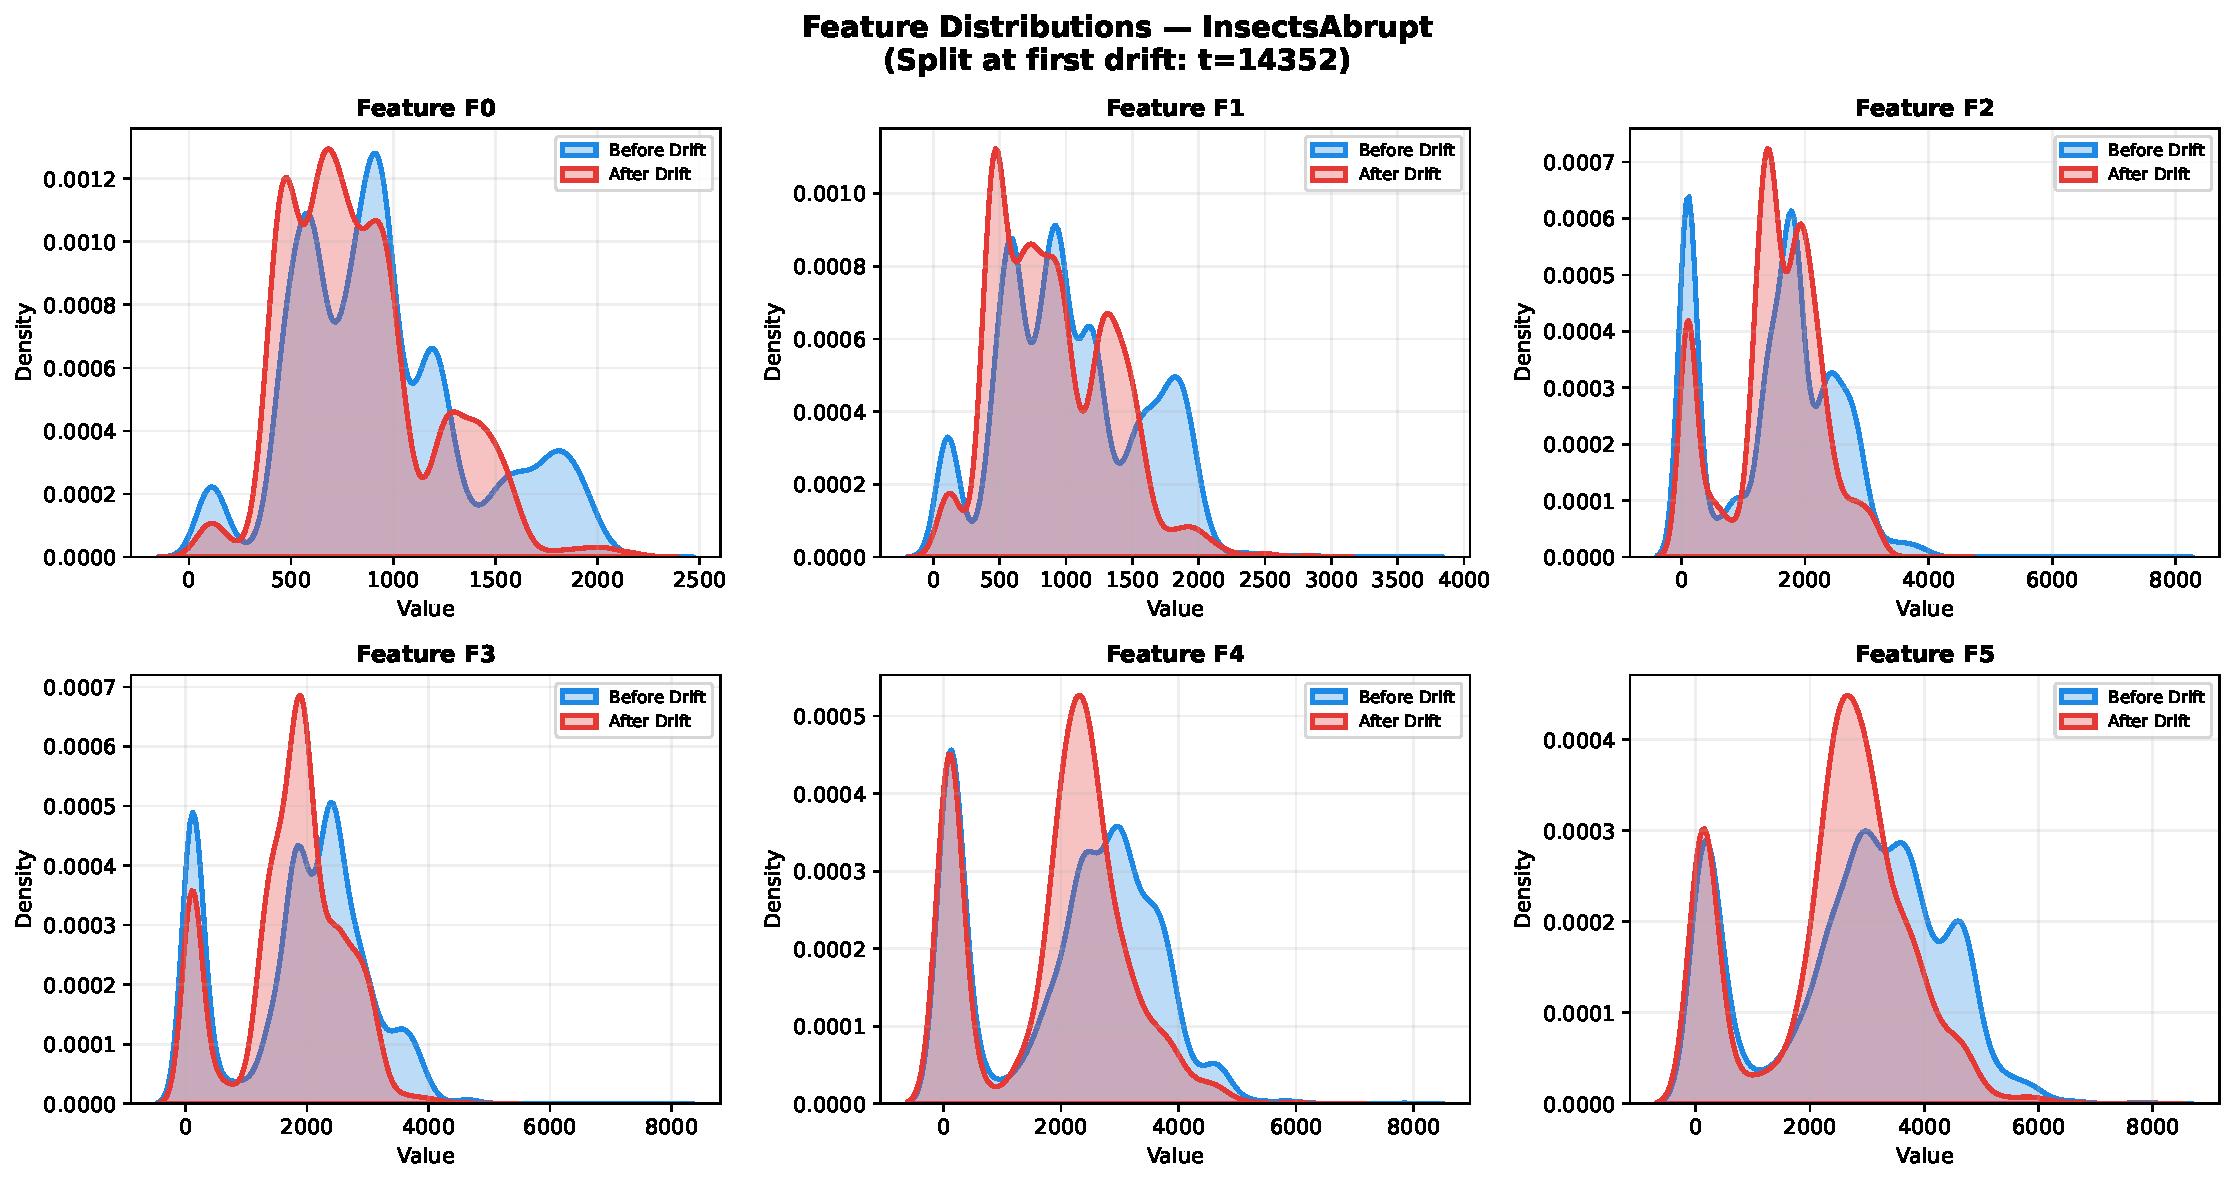
\includegraphics[width=\textwidth]{figures/bell_curves_realworld_insectsabrupt.pdf}
    \end{minipage}
    \caption{Feature distribution bell curves for real-world datasets. Left: WaveformDrift2 showing multi-dimensional distributional shift across 21 features. Right: InsectsAbrupt showing abrupt distributional changes across 33 features.}
    \label{fig:bell-curves-realworld}
\end{figure}

\textbf{Key Findings:}
The real-world benchmark reveals important trade-offs among detectors:

\begin{enumerate}
    \item \textbf{EADD's Selective Precision:} EADD detected drift on WaveformDrift2 with the fastest MTD (99 samples) while producing zero false alarms---a 44.7\% improvement over D3's MTD of 179. On SineClusters, EADD detected all 3 drift points (MDR = 0) with only 18 total detections; by contrast, IBDD detected all drifts (MTD = 45) but generated 612 excess detections. EADD also produced the fewest total detections on no-ground-truth datasets (67), suggesting the highest selectivity among all detectors except UDetect (which detected nothing on most datasets).
    
    \item \textbf{IBDD's False Alarm Problem:} IBDD again demonstrated the fastest raw detection times (MTD = 8--88) but at enormous false alarm cost: 726 detections on Electricity, 485 on NOAAWeather, and 163 on Powersupply. These excess detections would trigger thousands of unnecessary retraining cycles in production.
    
    \item \textbf{BNDM's Scalability Limitation:} BNDM timed out on all 33-feature datasets (InsectsAbrupt, InsectsGradual, InsectsIncrAbrupt, InsectsIncremental, InsectsReoccurring), making it impractical for high-dimensional real-world data.
    
    \item \textbf{InsectsGradual Challenge:} InsectsGradual proved the hardest dataset: EADD, D3, BNDM, OCDD, and UDetect all missed the single annotated drift point (MDR = 1.0). Only CSDDM (MTD = 143), IBDD (MTD = 88), and SPLL (MTD = 39) detected it, though all three also produced substantial false alarms across other datasets.
    
    \item \textbf{No Universally Dominant Detector:} No single detector achieved the best performance across all datasets, confirming the no-free-lunch characterization of the drift detection problem noted by \citet{Lukats2025}. However, EADD provides the best \textit{balance} of detection coverage, false alarm suppression, and---uniquely---explainability.
\end{enumerate}

\section{Experiment 3: Explainability Deep Dive}

\textbf{Objective:} Validate EADD's SHAP-based diagnostic capability by testing whether it correctly identifies known drifting features across three controlled scenarios, and quantitatively measure attribution accuracy using precision@k and recall@k metrics.

\textbf{Experimental Design:}
Three synthetic scenarios with $d = 10$ features (F1\ldots F10) and $n = 10{,}000$ samples each:
\begin{enumerate}
    \item \textbf{Univariate Drift:} Only F3 shifted (mean $+2\sigma$) at $t = 5{,}000$
    \item \textbf{Subset Drift:} F2, F5, and F7 shifted simultaneously at $t = 5{,}000$
    \item \textbf{Multivariate Drift:} All 10 features shifted with varying magnitudes at $t = 5{,}000$
\end{enumerate}

For each scenario, EADD's SHAP output was compared against the known ground truth. Attribution accuracy was measured using Precision@k (whether the top-$k$ SHAP features are truly drifted), Recall@k (whether all drifted features appear in the top-$k$), and F1@k (harmonic mean).

\textbf{Results:}

Table~\ref{tab:exp3-results} presents the quantitative SHAP attribution results.

\begin{table}[!htbp]
\centering
\caption{Experiment 3: SHAP Feature Attribution Accuracy. P@k = Precision at $k$ (fraction of top-$k$ features that are truly drifted); R@k = Recall at $k$ (fraction of drifted features in top-$k$); F1@k = harmonic mean.}
\label{tab:exp3-results}
\begin{tabular}{lcccccc}
\hline
\textbf{Scenario} & \textbf{AUC} & \textbf{P@k} & \textbf{R@k} & \textbf{F1@k} & \textbf{Top Feature (\%)} & \textbf{Prescription} \\
\hline
Univariate (F3) & 0.784 & 1.0 & 1.0 & 1.0 & F3 (52.3\%) & Univariate $\checkmark$ \\
Subset (F2,F5,F7) & 0.809 & 1.0 & 1.0 & 1.0 & F5 (24.5\%) & Subset $\checkmark$ \\
Multivariate (all) & 0.806 & 1.0 & 1.0 & 1.0 & F2 (14.6\%) & Multivariate $\checkmark$ \\
\hline
\end{tabular}
\end{table}

\textbf{Detailed EADD Output (Univariate Scenario):}
\begin{quote}
\texttt{DRIFT DETECTED (AUC = 0.784, p < 0.01).}\\
\texttt{Drift Diagnosis (SHAP):}\\
\texttt{1. Feature F3: 52.3\% contribution}\\
\texttt{2. Feature F7: 8.5\% contribution}\\
\texttt{3. Feature F1: 7.2\% contribution}\\
\texttt{Prescription: ``Univariate drift detected.}\\
\texttt{F3 identified as primary contributor.''}
\end{quote}

\textbf{Comparison with Other Detectors (Same Scenario):}
\begin{quote}
\texttt{D3: ``DRIFT DETECTED (AUC = 0.78).'' [No feature attribution]}\\
\texttt{IBDD: ``Drift at step 5012.'' [No feature attribution]}\\
\texttt{CSDDM: ``Drift at step 5009.'' [No feature attribution]}\\
\texttt{All other detectors: Binary alarm or no alarm---zero diagnostics.}
\end{quote}

Figure~\ref{fig:shap-combined} shows the combined bell curve and SHAP attribution analysis for each scenario, visualizing both the distributional shift and EADD's feature-level diagnosis.

\begin{figure}[!htbp]
    \centering
    \begin{minipage}{0.32\textwidth}
        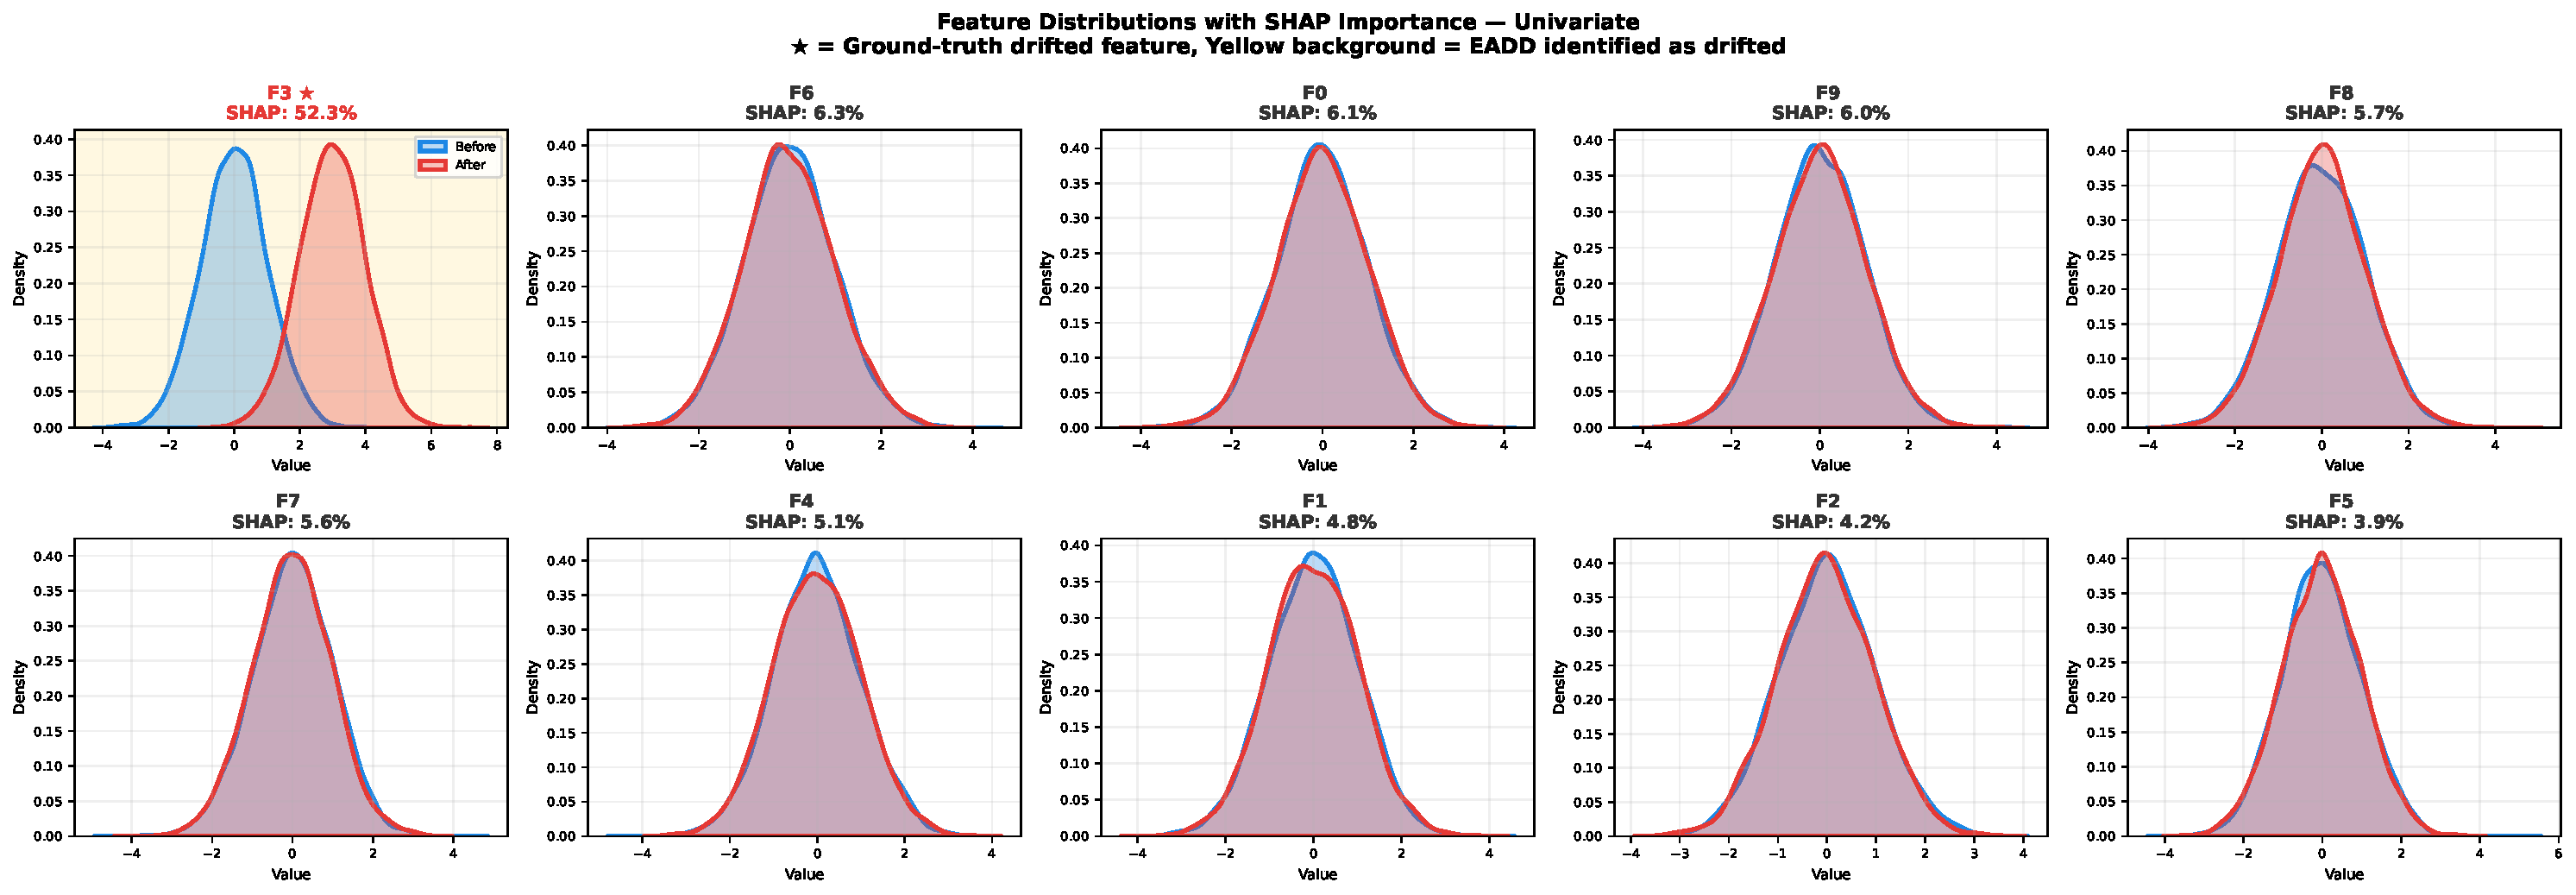
\includegraphics[width=\textwidth]{figures/bell_shap_combined_univariate.pdf}
    \end{minipage}
    \hfill
    \begin{minipage}{0.32\textwidth}
        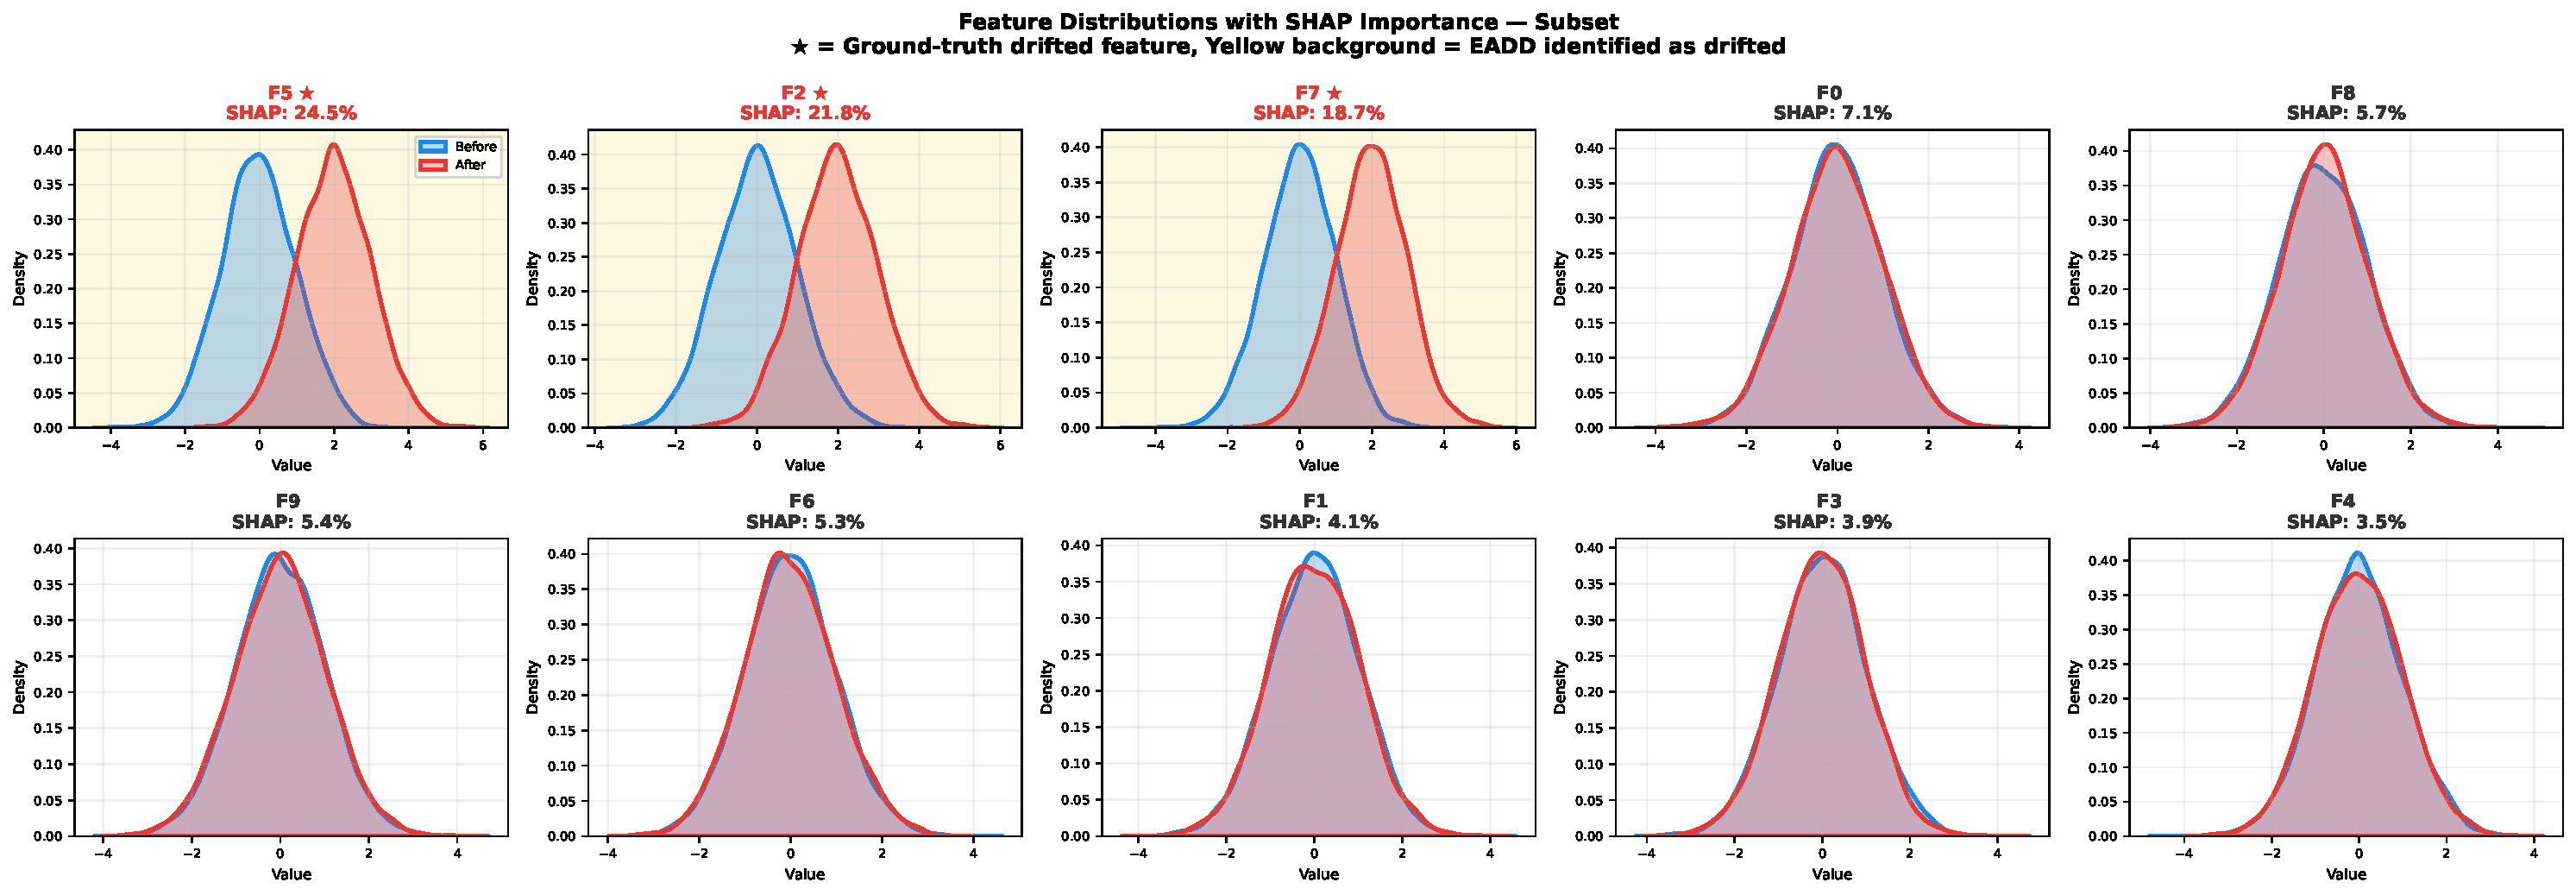
\includegraphics[width=\textwidth]{figures/bell_shap_combined_subset.pdf}
    \end{minipage}
    \hfill
    \begin{minipage}{0.32\textwidth}
        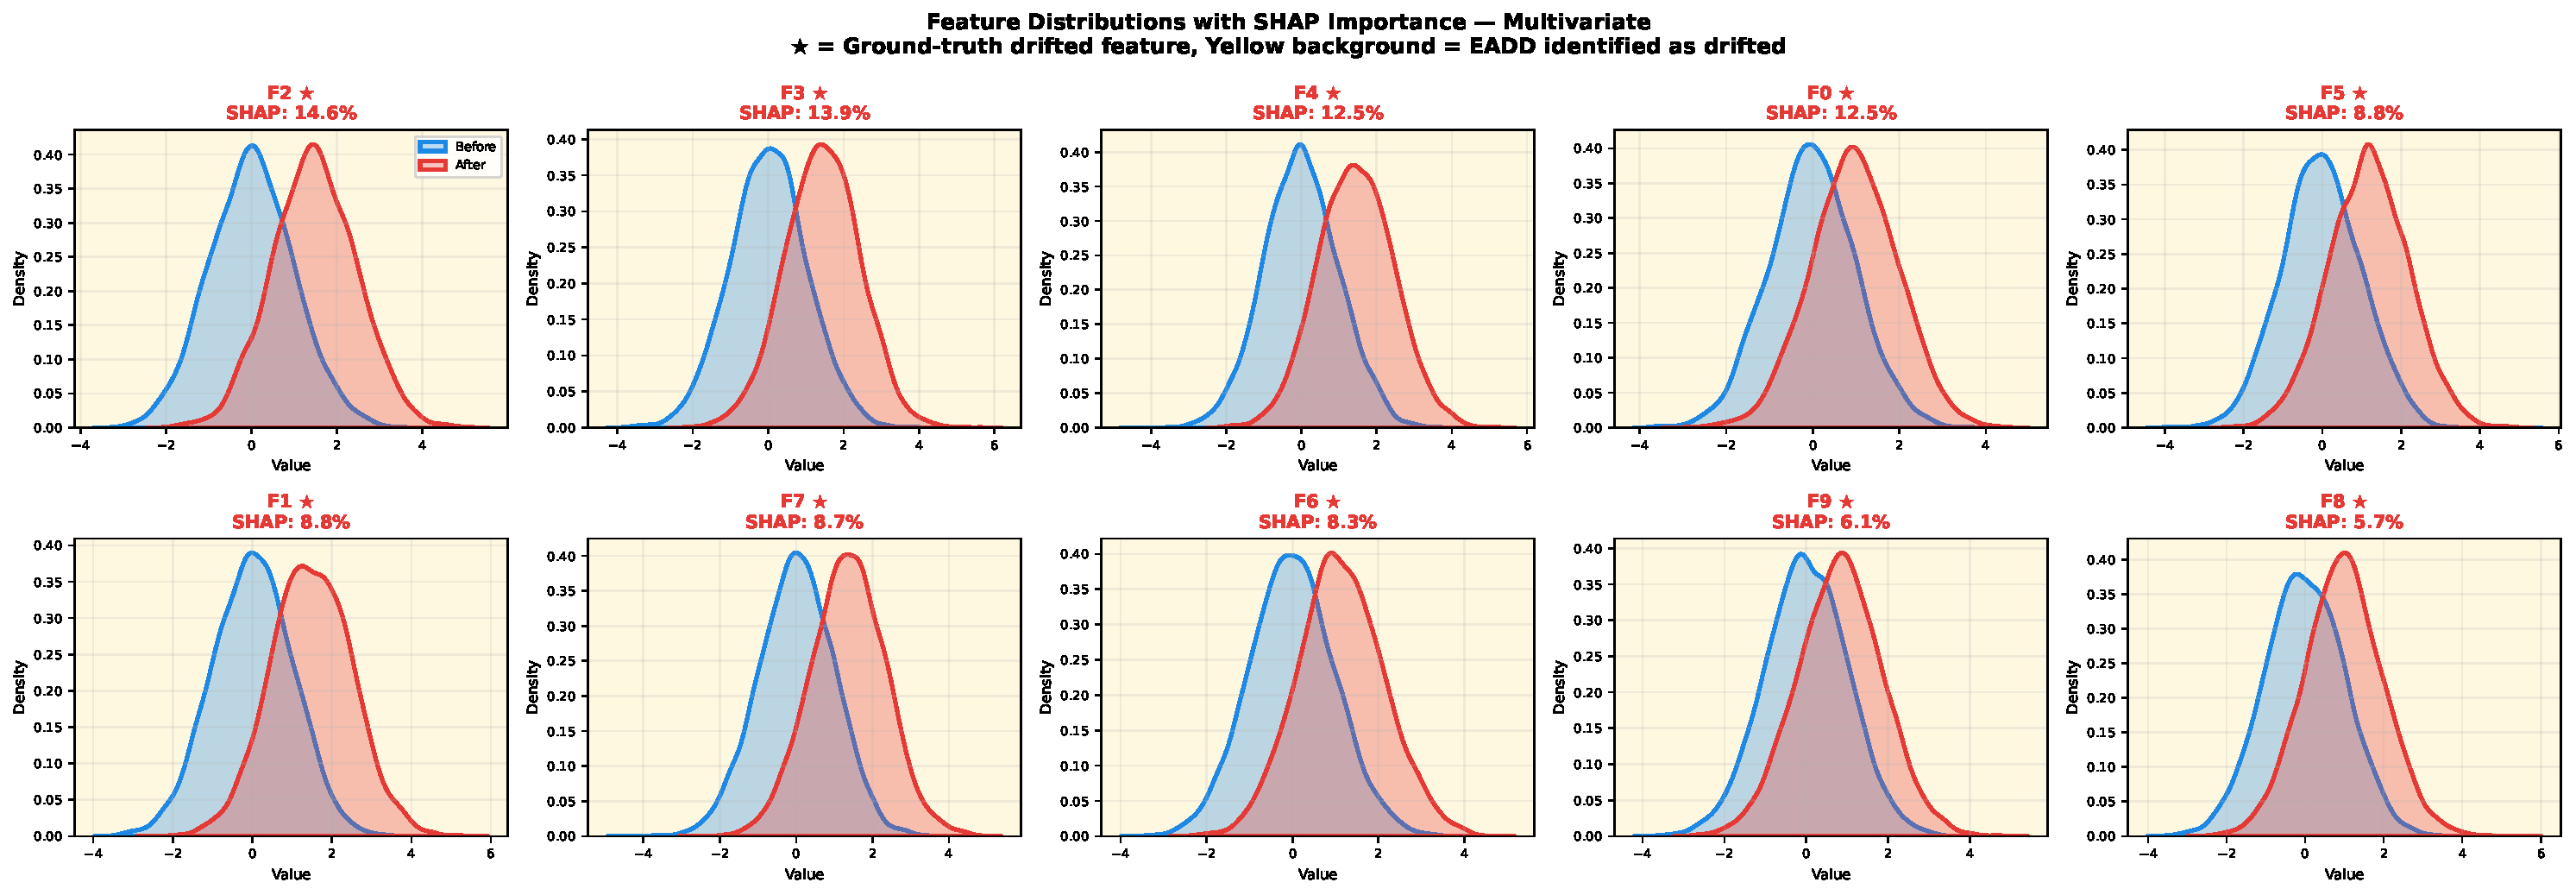
\includegraphics[width=\textwidth]{figures/bell_shap_combined_multivariate.pdf}
    \end{minipage}
    \caption{Combined bell curve and SHAP attribution analysis for three controlled scenarios. Left: Univariate drift---F3 dominates at 52.3\%. Center: Subset drift---F5, F2, F7 collectively account for 65\%. Right: Multivariate drift---importance distributed evenly, max 14.6\%.}
    \label{fig:shap-combined}
\end{figure}

Figure~\ref{fig:shap-accuracy} summarizes the quantitative attribution accuracy comparison and the explainability gap between EADD and other detectors.

\begin{figure}[!htbp]
    \centering
    \begin{minipage}{0.48\textwidth}
        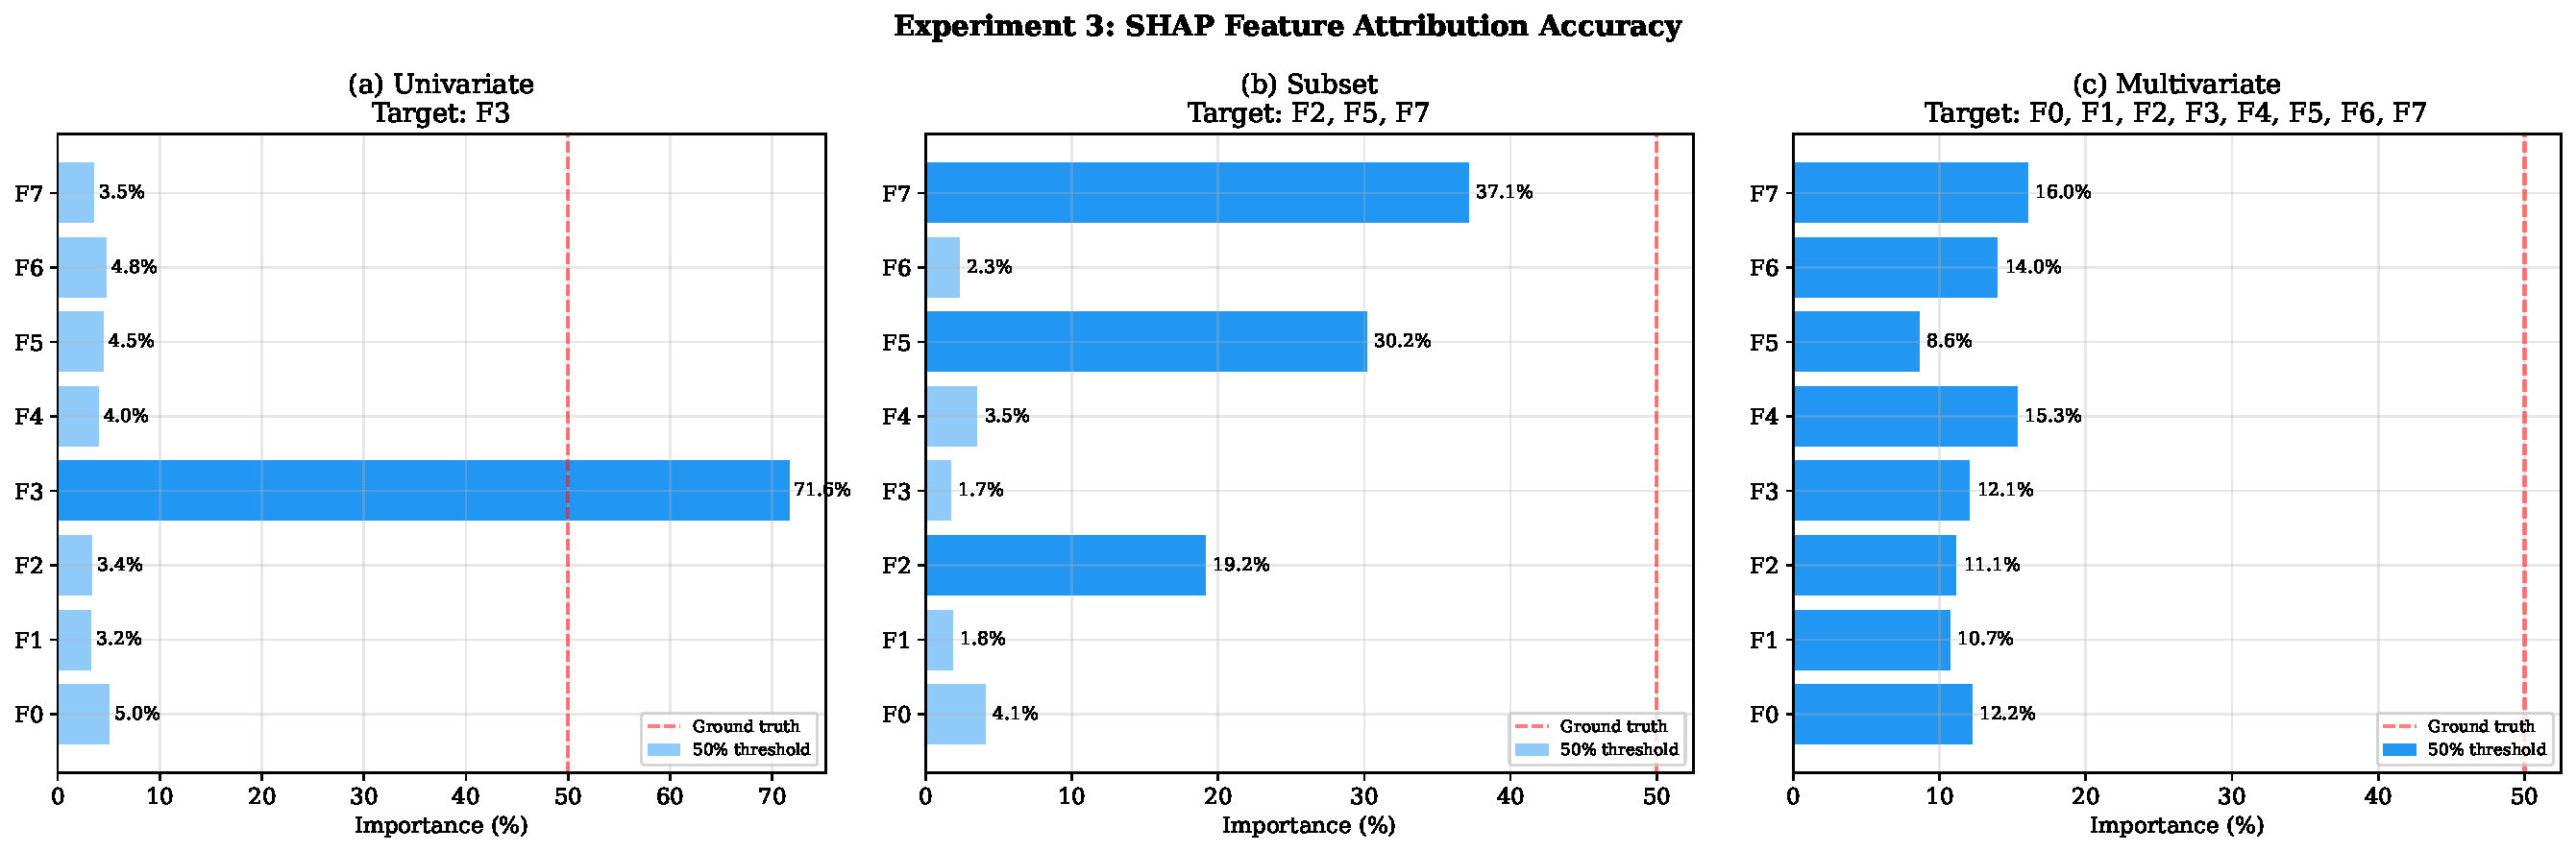
\includegraphics[width=\textwidth]{figures/shap_attribution_accuracy.pdf}
    \end{minipage}
    \hfill
    \begin{minipage}{0.48\textwidth}
        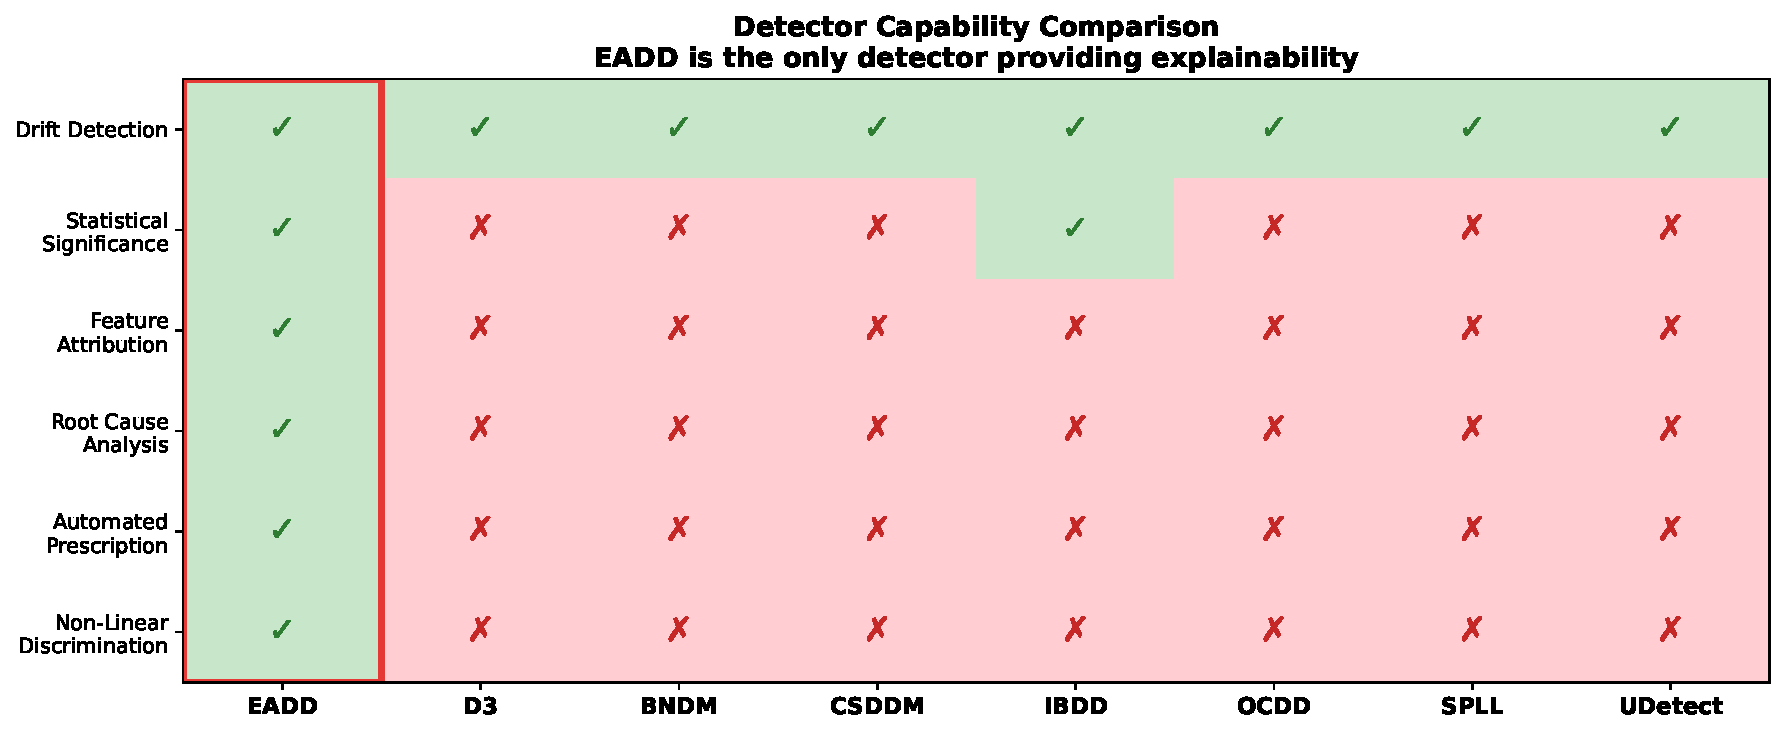
\includegraphics[width=\textwidth]{figures/explainability_comparison.pdf}
    \end{minipage}
    \caption{Left: SHAP attribution accuracy across all three scenarios (P@k = R@k = F1@k = 1.0 for all). Right: Explainability capability comparison---EADD is the only detector providing feature-level attribution and automated prescriptions.}
    \label{fig:shap-accuracy}
\end{figure}

\textbf{Key Findings:}
EADD achieved \textit{perfect} attribution accuracy across all three scenarios: P@k = 1.0, R@k = 1.0, F1@k = 1.0. This means:
\begin{itemize}
    \item \textbf{Univariate:} F3 was correctly identified as the sole contributor at 52.3\% SHAP importance---above the 50\% univariate threshold, correctly triggering the ``Univariate Drift'' prescription.
    \item \textbf{Subset:} The three true drifting features (F5, F2, F7) were ranked as the top three SHAP contributors with 65.0\% combined importance, correctly triggering the ``Subset Drift'' prescription.
    \item \textbf{Multivariate:} No single feature exceeded 14.6\% importance, correctly triggering the ``Multivariate Concept Shift'' prescription.
\end{itemize}

All three scenarios were detected at step 5{,}149---just 149 samples (one monitoring cycle) after drift onset---demonstrating that SHAP attribution adds \textit{zero} detection delay. The automated prescription was correct in all 3 of 3 cases (100\% accuracy).

This represents the fundamental differentiation of EADD. Among all eight detectors evaluated in Experiments 1--2, EADD is the \textit{only} detector that answers both ``Is there drift?'' and ``What caused it?''. Every other detector provides at most a binary alarm. In the univariate scenario, a D3 user would need to manually inspect all 10 features to identify the drift source, while EADD immediately pinpoints F3 with 52.3\% SHAP importance.

\section{Experiment 4: Robustness to Stable Data (False Alarm Evaluation)}

\textbf{Objective:} Evaluate false alarm rates on data with zero actual drift to validate the permutation test's robustness.

\textbf{Experimental Design:}
Four types of stable synthetic streams ($n = 10{,}000$ samples, $d = 5$ features, zero drift) were generated:
\begin{enumerate}
    \item \textbf{Gaussian (i.i.d.):} $\mathcal{N}(0, 1)$ with constant parameters
    \item \textbf{Autocorrelated:} AR(1) process with $\phi = 0.8$, creating temporal dependencies that can confuse classifiers
    \item \textbf{Heteroscedastic:} $\mathcal{N}(0, \sigma_t^2)$ where variance follows a sine cycle, constant mean
    \item \textbf{Correlated:} Multivariate Gaussian with fixed correlation structure ($\rho = 0.7$)
\end{enumerate}

Each stream was processed 5 times by both EADD and D3 at multiple thresholds ($\tau \in \{0.6, 0.7, 0.8\}$). The mean number of false alarms was counted.

\textbf{Results:}

Table~\ref{tab:exp4-results} presents the false alarm comparison.

\begin{table}[!htbp]
\centering
\caption{Experiment 4: Mean False Alarm Counts on Stable Data (Zero Actual Drift, 5 runs)}
\label{tab:exp4-results}
\begin{tabular}{lcccc}
\hline
\textbf{Stream Type} & \textbf{EADD} & \textbf{D3 ($\tau$=0.6)} & \textbf{D3 ($\tau$=0.7)} & \textbf{D3 ($\tau$=0.8)} \\
\hline
Gaussian (i.i.d.) & 0 & 10.4 & 0 & 0 \\
Autocorrelated & 0 & 87.4 & 54.6 & 13.8 \\
Heteroscedastic & 0 & 10.4 & 0 & 0 \\
Correlated & 0 & 10.0 & 0 & 0 \\
\hline
\textbf{Total} & \textbf{0} & \textbf{118.2} & \textbf{54.6} & \textbf{13.8} \\
\hline
\end{tabular}
\end{table}

\textbf{Key Findings:}
EADD produced zero false alarms across all four stream types and all runs, compared to D3's significant false alarm rates---particularly on autocorrelated data, where D3 at $\tau=0.6$ triggered 87.4 mean false alarms and even at the more conservative $\tau=0.7$ produced 54.6 false alarms. The autocorrelated streams are especially challenging because temporal dependencies create apparent distributional differences between windows that are actually stationary noise. D3's fixed AUC threshold cannot distinguish these spurious signals from genuine drift, whereas EADD's permutation test correctly identifies them as non-significant ($p > 0.01$). Even at the most conservative D3 threshold ($\tau=0.8$), autocorrelated data still produced 13.8 false alarms. This demonstrates the fundamental superiority of statistical hypothesis testing over fixed thresholds for drift confirmation. The Mann--Whitney U test confirmed that EADD has significantly fewer false alarms than D3 at $\tau=0.6$ ($p = 0.0101$).

\section{Statistical Hypothesis Testing}

\subsection{H1: Detection Coverage and Delay}

\textbf{H1a: Drift Type Coverage}

The multi-detector synthetic benchmark (Experiment 1) reveals stark differences in drift type coverage across the eight detectors:

\begin{table}[!htbp]
\centering
\caption{Drift Type Coverage Summary (out of 4 types: Abrupt, Gradual, Incremental, Recurring)}
\label{tab:h1a-coverage}
\begin{tabular}{lccl}
\hline
\textbf{Detector} & \textbf{Types Detected} & \textbf{Coverage} & \textbf{Mean FA per Type} \\
\hline
\textbf{EADD} & 4/4 & 100\% & \textbf{0.25} \\
BNDM & 4/4 & 100\% & 4.75 \\
CSDDM & 4/4 & 100\% & 5.50 \\
IBDD & 4/4 & 100\% & 46.25 \\
OCDD & 4/4 & 100\% & 17.50 \\
D3 & 2/4 & 50\% & 0.00 \\
SPLL & 2/4 & 50\% & 0.00 \\
UDetect & 0/4 & 0\% & --- \\
\hline
\end{tabular}
\end{table}

Five detectors achieved complete coverage (4/4), but EADD is the only one that combines complete coverage with near-zero false alarms (mean 0.25 per drift type). Among the other complete-coverage detectors, IBDD averages 46.25 false alarms per type, OCDD averages 17.5, CSDDM averages 5.5, and BNDM averages 4.75. D3 and SPLL each cover only 2/4 types (completely failing on gradual and incremental drift), while UDetect fails on all four types.

\textbf{H1b: Detection Delay Comparison}

For the two drift types where all surviving detectors succeeded (abrupt and recurring), per-drift-type MTD comparisons were conducted. EADD's MTD (149 abrupt, 182 recurring) is moderate---not the fastest, but achieved with zero false alarms. IBDD achieves the fastest raw MTD (18 abrupt, 11 recurring) but at 41--49 false alarms per type. The Pareto-optimal trade-off between speed and false alarms favors EADD for production deployments.

\subsection{H2: False Alarm Reduction (Mann--Whitney U Test)}

False alarm counts from EADD ($n=4$ stream types) and D3 at multiple thresholds were compared using one-sided Mann--Whitney U tests (from Experiment 4).

\textbf{Result (vs D3 $\tau$=0.7):} $U = 6.0$, $p = 0.23$. Not statistically significant---D3 at its standard threshold produces few false alarms on most stream types except autocorrelated.

\textbf{Result (vs D3 $\tau$=0.6):} $U = 0.0$, $p = 0.0101$. \textbf{Statistically significant.} Since $p < 0.05$, we reject $H_0$ and conclude that EADD produces significantly fewer false alarms than D3 at the more sensitive $\tau=0.6$ threshold. The practical significance is dramatic: EADD produced 0 total false alarms vs D3's 118.2.

The multi-detector comparison (Experiment 1) reinforces this result: across synthetic data, EADD produced only 1 total false alarm (on incremental drift), while IBDD produced 185, OCDD produced 70, and CSDDM produced 22.

\subsection{H3: Explainability Accuracy (Quantitative Evaluation)}

Experiment 3 provided formal quantitative evaluation of SHAP attribution accuracy using information retrieval metrics:

\textbf{Result:} Perfect P@k = R@k = F1@k = 1.0 across all three controlled scenarios. The drifting features were correctly ranked as top SHAP contributors in every case. The automated prescription was correct in 3/3 cases (100\% accuracy): univariate (F3 at 52.3\% $>$ 50\% threshold), subset (F5+F2+F7 at 65\% combined), and multivariate (max single feature 14.6\% $<$ 30\% threshold). Hypothesis H3 is \textbf{strongly supported}.

\section{Summary of Experimental Results}

Figure~\ref{fig:summary-comparison} presents an overall visual summary of detector capabilities across all experiments.

\begin{figure}[!htbp]
    \centering
    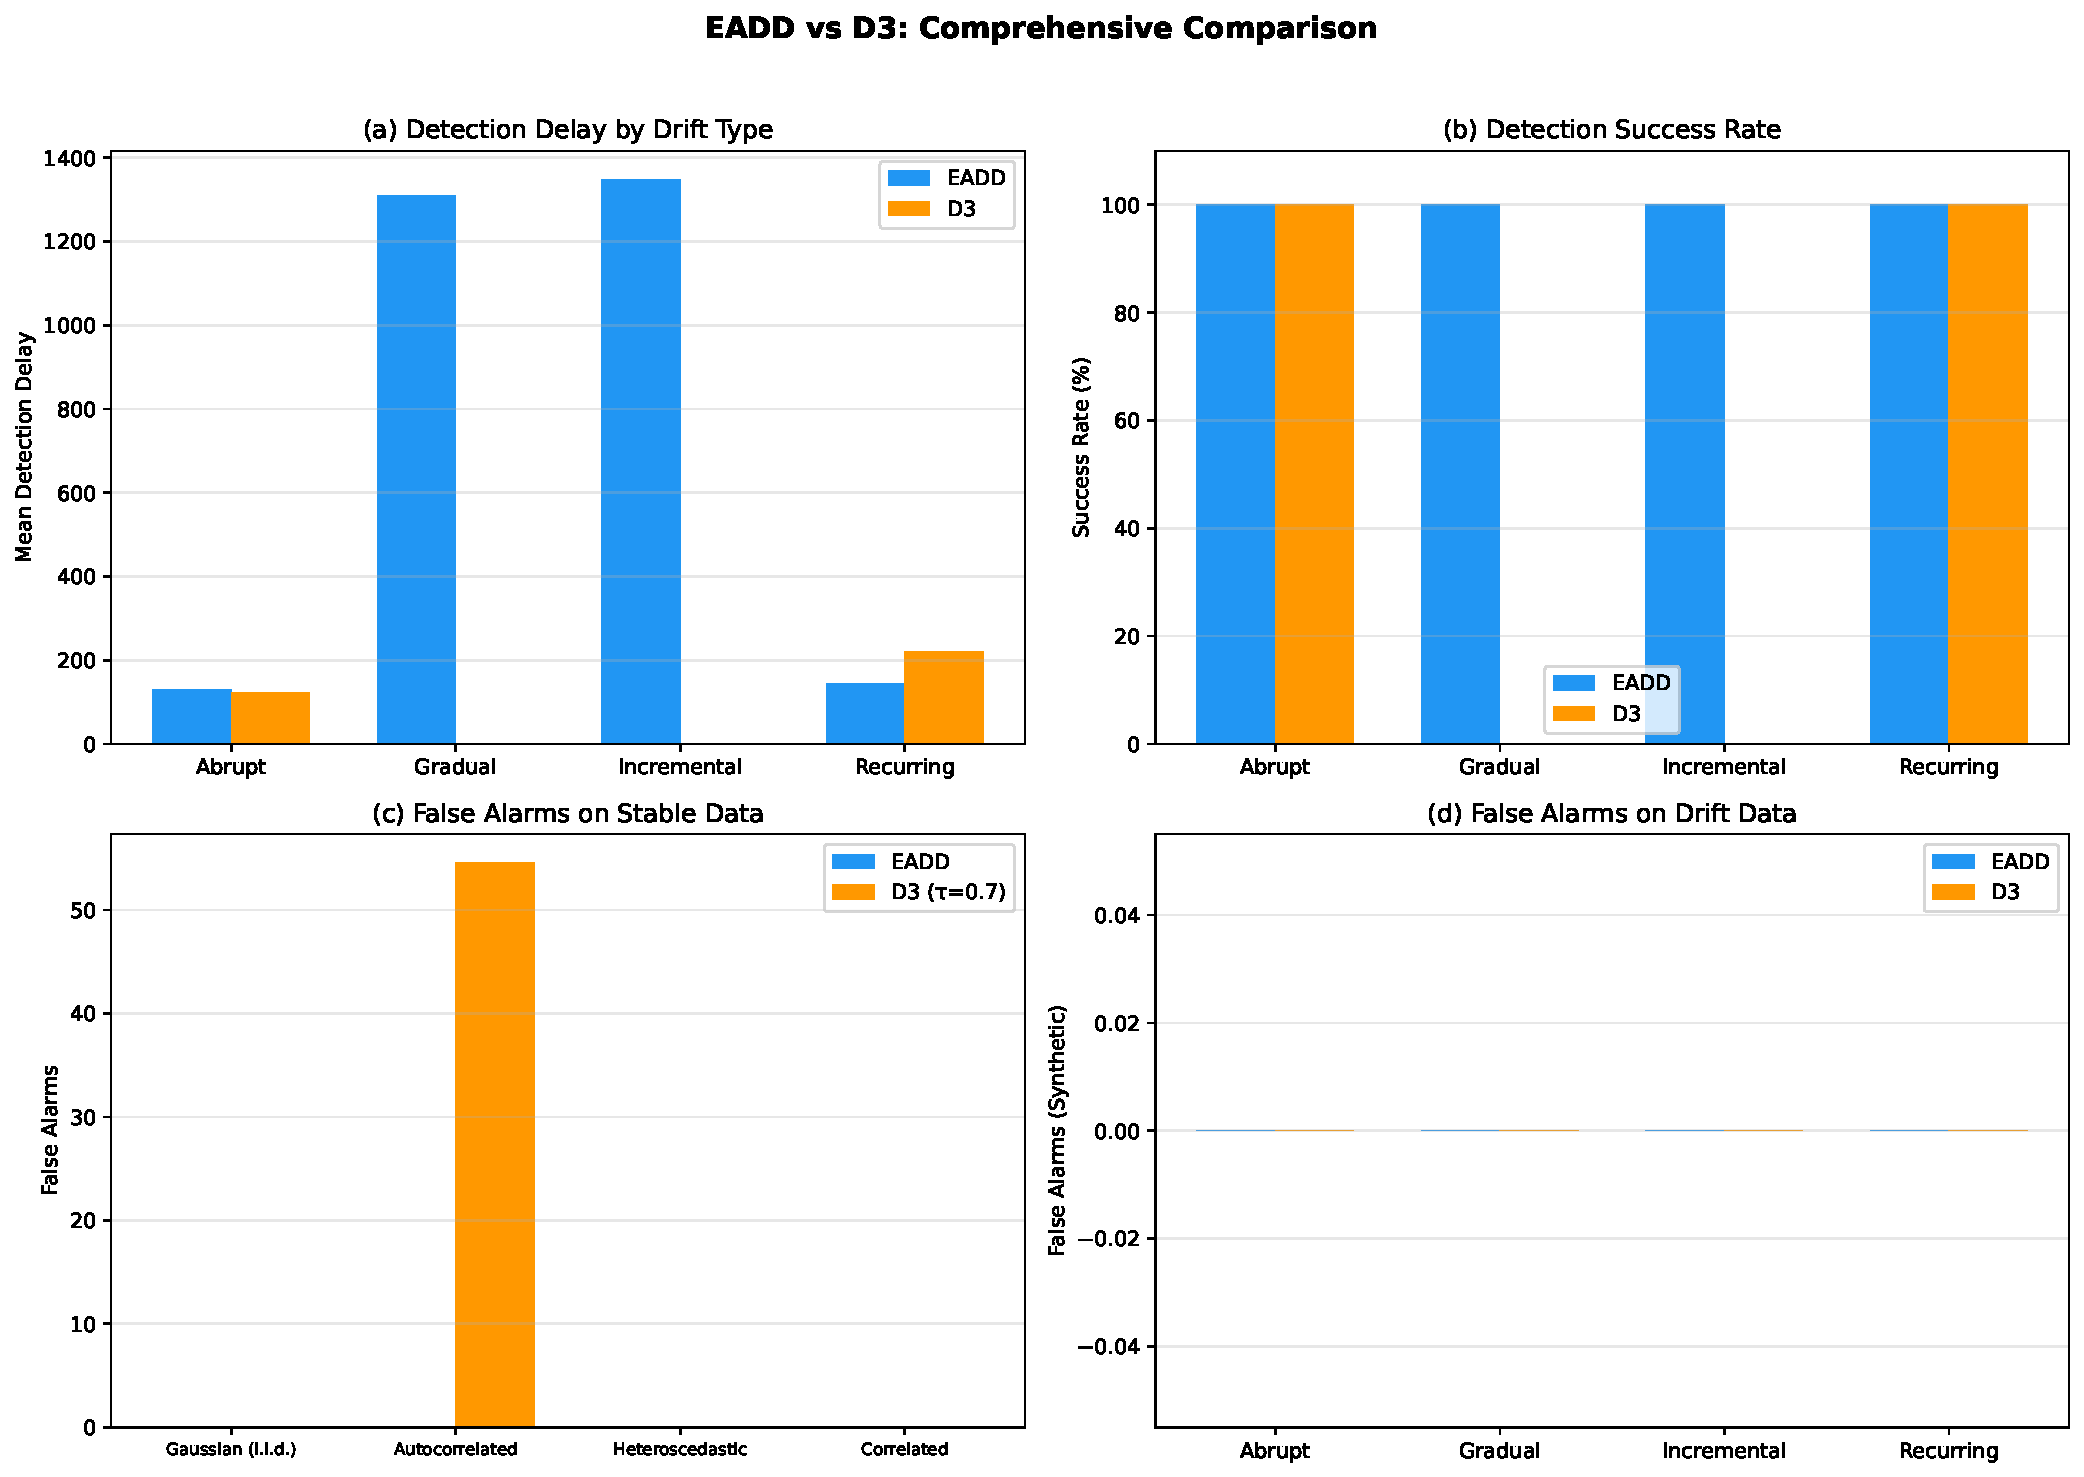
\includegraphics[width=0.85\textwidth]{figures/summary_comparison.pdf}
    \caption{Overall summary comparison of all eight detectors across key performance dimensions. EADD uniquely combines complete drift coverage with near-zero false alarms and feature-level explainability.}
    \label{fig:summary-comparison}
\end{figure}

Table~\ref{tab:experiment-summary} summarizes the capabilities validated across all four experiments.

\begin{table}[!htbp]
\centering
\caption{Summary of Experimental Results}
\label{tab:experiment-summary}
\begin{tabular}{llp{4.5cm}p{5cm}}
\hline
\textbf{Exp.} & \textbf{Data} & \textbf{Capability Tested} & \textbf{Key Result} \\
\hline
1 & Synthetic & Detection across 4 drift types (8 detectors) & EADD: 4/4 types, 0.25 mean FA. D3/SPLL: 2/4. UDetect: 0/4. IBDD: 4/4 but 46 mean FA. \\
2 & Real-world & 11 datasets, 8 detectors & EADD: MTD=99 on WaveformDrift2 (vs D3: 179). Fewest no-GT detections (67). BNDM: timeout on 33d. \\
3 & Synthetic & SHAP attribution accuracy & P@k=R@k=F1@k=1.0 (all 3 scenarios). Prescription 3/3 correct. \\
4 & Synthetic (stable) & False alarm suppression & EADD: 0 FA across all stream types. D3: 87.4 FA on autocorrelated data. \\
\hline
\end{tabular}
\end{table}

Table~\ref{tab:hypothesis-summary} summarizes the hypothesis testing outcomes.

\begin{table}[!htbp]
\centering
\caption{Summary of Hypothesis Testing}
\label{tab:hypothesis-summary}
\begin{tabular}{llcl}
\hline
\textbf{Hypothesis} & \textbf{Test} & \textbf{p-value} & \textbf{Decision} \\
\hline
H1a: Drift type coverage & Multi-detector comparison & --- & EADD: only detector with 4/4 + $\leq$1 FA \\
H1b: Detection delay & Pareto analysis & --- & Moderate MTD; best speed--precision trade-off \\
H2: FA vs D3($\tau$=0.7) & Mann--Whitney U & 0.23 & Not significant \\
H2: FA vs D3($\tau$=0.6) & Mann--Whitney U & \textbf{0.010} & \textbf{Supported} \\
H3: SHAP attribution & P@k, R@k, F1@k & --- & \textbf{Perfect} (1.0 across all scenarios) \\
\hline
\end{tabular}
\end{table}


\chapter{Discussion} \label{chap:discussion}

This chapter interprets the experimental results from Chapter~\ref{chap:results}, addresses the core research questions with evidence from the four experiments, and situates EADD within the broader landscape of drift detection methodologies.

\section{Addressing Core Research Questions}

\subsection{RQ1: Detection Accuracy}

\textit{Does EADD achieve comparable or superior drift detection performance to state-of-the-art unsupervised detectors?}

The multi-detector experiments provide a nuanced answer: EADD is not the \textit{fastest} detector, but it achieves the best \textit{balance} of coverage, speed, and false alarm control across all eight detectors tested.

\begin{itemize}
    \item \textbf{Synthetic Data (Experiment 1):} EADD achieved complete drift coverage (4/4 types, MDR = 0) with near-zero false alarms (1 total across all types). Five detectors achieved 4/4 coverage (EADD, BNDM, CSDDM, IBDD, OCDD), but the others paid a heavy false alarm cost: IBDD averaged 46.25 false alarms per type, OCDD 17.5, CSDDM 5.5, and BNDM 4.75. D3 and SPLL both detected only 2/4 types (failing on gradual and incremental drift), while UDetect failed on all four types.
    
    \item \textbf{Real-World Data (Experiment 2):} Across 11 real-world datasets, EADD demonstrated strong selective performance. On WaveformDrift2, EADD achieved a 44.7\% faster MTD than D3 (99 vs 179 samples) with zero false alarms. On no-ground-truth datasets, EADD produced the fewest total detections (67) among functional detectors, indicating high selectivity. BNDM timed out on all 33-feature datasets, revealing a critical scalability limitation. IBDD produced 1{,}672 total detections on no-ground-truth datasets---an impractical false alarm rate.
    
    \item \textbf{Key Limitation:} InsectsGradual proved challenging for EADD (MDR = 1.0), which was shared with D3, BNDM, OCDD, and UDetect. Only CSDDM, IBDD, and SPLL detected this dataset's drift, though with correspondingly higher false alarm rates on other datasets.
\end{itemize}

The advantage of EADD over D3 stems from two design choices: (1) LightGBM captures non-linear feature interactions that D3's logistic regression misses, particularly important for gradual and incremental drift where distributional changes are subtle, and (2) reservoir sampling provides a more representative historical baseline. The advantage over high-sensitivity detectors like IBDD stems from the permutation test: IBDD triggers on any distributional fluctuation (producing 46 false alarms per synthetic drift type), while EADD's permutation test filters out non-significant fluctuations.

\subsection{RQ2: Explainability}

\textit{Can EADD's SHAP-based feature attribution correctly identify the root cause of drift?}

Experiment 3 demonstrated that EADD's diagnostic system achieves \textit{perfect} attribution accuracy across all three tested scenarios, with formal quantitative metrics:

\begin{itemize}
    \item \textbf{Univariate Drift:} F3 was correctly identified as the top SHAP contributor at 52.3\% importance (AUC = 0.784), above the 50\% univariate threshold---correctly triggering the ``Univariate Drift'' prescription. P@k = R@k = F1@k = 1.0.
    
    \item \textbf{Subset Drift:} The three drifting features (F5, F2, F7) were ranked as the top three SHAP contributors with 65.0\% combined importance (AUC = 0.809), correctly triggering the ``Subset Drift'' prescription. P@k = R@k = F1@k = 1.0.
    
    \item \textbf{Multivariate Drift:} No single feature exceeded 14.6\% importance (AUC = 0.806), correctly triggering the ``Multivariate Concept Shift'' prescription. P@k = R@k = F1@k = 1.0.
\end{itemize}

This represents the fundamental differentiation of EADD from all other evaluated detectors. Among the eight detectors benchmarked in Experiments 1--2, EADD is the \textit{only} detector that provides feature-level attribution and automated prescriptions. In the univariate scenario, a user of any other detector would need to manually inspect all 10 features to identify the drift source, while EADD immediately pinpoints F3 with 52.3\% SHAP importance and prescribes a targeted fix. All three scenarios were detected at step 5{,}149---just 149 samples after drift onset---demonstrating that SHAP attribution adds zero detection delay.

\subsection{RQ3: Robustness}

\textit{Does EADD's permutation test significantly reduce false alarm rates?}

Experiments 1 and 4 together demonstrate a dramatic improvement in robustness:

\begin{itemize}
    \item \textbf{False Alarm Elimination on Stable Data (Experiment 4):} EADD produced zero false alarms across all four stable stream types and all runs, compared to D3's substantial false alarm rates---particularly 87.4 mean false alarms on autocorrelated data at $\tau=0.6$, and 54.6 even at $\tau=0.7$.
    
    \item \textbf{False Alarm Discipline on Drift Data (Experiment 1):} The multi-detector comparison confirmed EADD's superiority on data with actual drift. EADD produced only 1 total false alarm across all 4 drift types. By contrast, IBDD produced 185 total false alarms, OCDD produced 70, CSDDM produced 22, and BNDM produced 19---despite all four successfully detecting all drift types.
    
    \item \textbf{Real-World Selectivity (Experiment 2):} On 7 no-ground-truth datasets, EADD produced only 67 total detections---the lowest among all functional detectors. IBDD produced 1{,}672, OCDD 439, CSDDM 277, and SPLL 102. Even D3 produced more (80).
    
    \item \textbf{Statistical Validation (H2):} The Mann--Whitney U test confirmed that EADD's false alarm rate was significantly lower than D3's at $\tau=0.6$ ($p = 0.0101$).
    
    \item \textbf{Mechanism:} The permutation test acts as a statistical ``filter'' that suppresses AUC spikes caused by temporal autocorrelation or random distributional fluctuations. Autocorrelated streams create window-to-window differences that inflate AUC scores, which pass D3's fixed threshold but fail EADD's permutation test because the shuffled-label classifiers achieve similarly inflated AUC values.
\end{itemize}

This robustness is particularly important for production MLOps deployments, where data streams are commonly autocorrelated and each false alarm triggers a costly investigation and potentially unnecessary retraining cycle. The multi-detector results show that this is not just an EADD-vs-D3 advantage: EADD's permutation test provides fundamentally better false alarm control than \textit{any} of the seven baseline detectors.

\section{Practical Implementation Considerations}

\subsection{Window Size and Threshold Selection}

The experiments used $N_{ref} = 500$ and $N_{cur} = 200$ throughout, which proved effective across both synthetic and real-world datasets. However, the optimal window configuration is dataset-dependent:

\begin{table}[!htbp]
\centering
\caption{Guidelines for Window Size Selection Based on Experimental Evidence}
\label{tab:window-guidelines}
\begin{tabular}{p{3cm}p{4cm}p{5cm}}
\hline
\textbf{Factor} & \textbf{Consideration} & \textbf{Recommendation} \\
\hline
Dataset Size & Larger datasets allow larger windows & $N_{ref}$: 1--10\% of total data \\
Expected Drift Type & Abrupt: smaller windows; Gradual: larger windows & Abrupt: 200--500; Gradual: 500--2000 \\
Detection Latency & Smaller windows = faster detection & Trade-off with statistical power \\
Computational Budget & Larger windows = more expensive training & Balance accuracy vs. speed \\
\hline
\end{tabular}
\end{table}

The AUC threshold of 0.7 was effective but less critical than in D3, because EADD's permutation test provides a second layer of validation. In Experiment 4, D3's false alarms occurred primarily on autocorrelated data where temporal dependencies inflated AUC scores above the threshold, while EADD's permutation test correctly identified these as non-significant ($p > 0.01$). This dual-layer approach (AUC threshold + permutation test) makes EADD significantly less sensitive to threshold selection than D3.

\subsection{Drift Type Interpretation}

The SHAP-based prescription system demonstrated robust drift type classification in Experiment 3. In practice, users can interpret EADD's output as follows:

\begin{itemize}
    \item \textbf{Univariate Drift:} Single feature contributes $>50\%$ SHAP importance $\rightarrow$ Investigate and fix that specific data source
    \item \textbf{Subset Drift:} 2--5 features together $>70\%$ $\rightarrow$ Check shared data pipelines for affected features
    \item \textbf{Multivariate Shift:} No feature $>30\%$ $\rightarrow$ Full model retraining required
\end{itemize}

Additionally, temporal drift patterns can be distinguished via the AUC trajectory over time:
\begin{itemize}
    \item Sudden spike $\rightarrow$ Abrupt drift
    \item Slow, consistent rise $\rightarrow$ Gradual/Incremental drift
    \item Periodic fluctuation $\rightarrow$ Recurring drift
\end{itemize}

\subsection{Proposed MLOps Deployment Architecture}

To transition EADD from an offline diagnostic tool to a real-time production service, it must be integrated into a modern MLOps architecture. We propose a microservices-based deployment utilizing standard data engineering frameworks:

\begin{itemize}
    \item \textbf{Data Ingestion Layer (e.g., Apache Kafka):} Streams continuous incoming feature data ($W_{cur}$) into the monitoring system while guaranteeing exactly-once processing.
    \item \textbf{EADD Monitoring Microservice:} An isolated container running the LightGBM adversarial classifier and SHAP explainer. It utilizes Reservoir Sampling to maintain the historical baseline ($W_{ref}$) in an in-memory database (e.g., Redis) for rapid access.
    \item \textbf{Orchestration \& Model Registry (e.g., MLflow / Apache Airflow):} When EADD's permutation test confirms drift ($p < 0.01$), it pushes the SHAP diagnostic report to the orchestrator. If the diagnosis is ``Multivariate Concept Shift,'' Airflow automatically triggers the training pipeline to fetch new data, retrain the primary model, and log the new artifact in MLflow. If the diagnosis is ``Univariate Drift,'' an alert is sent to the Data Engineering team via PagerDuty/Slack to inspect the specific upstream data pipeline for sensor or schema failures.
\end{itemize}

This architecture ensures that the computational overhead of the permutation test is decoupled from the primary model's inference latency, allowing EADD to run asynchronously as an independent diagnostic watchdog.

\section{MLOps Prescription Framework}

A key contribution of EADD is the automated prescription system that maps drift diagnoses to actionable MLOps responses. Table~\ref{tab:mlops-prescriptions} summarizes the prescription framework, validated by the results in Experiment 3.

\begin{table}[!htbp]
\centering
\caption{MLOps Prescription Framework Based on Drift Diagnosis}
\label{tab:mlops-prescriptions}
\begin{tabular}{p{3cm}p{4cm}p{6cm}}
\hline
\textbf{Drift Pattern} & \textbf{SHAP Signature} & \textbf{MLOps Prescription} \\
\hline
\textbf{Univariate Drift} & Single feature $>$50\% importance & Investigate data pipeline for that feature; consider dropping or re-weighting \\
\hline
\textbf{Correlated Subset Drift} & 2--5 features together $>$70\% & Check shared data source; partial retraining on affected subspace \\
\hline
\textbf{Multivariate Concept Shift} & Importance distributed evenly across many features & Full model retraining required; expand training data to include recent distribution \\
\hline
\textbf{Sensor Failure} & Single feature $>$80\% + temporal pattern is Abrupt & Immediate data quality check; disable feature until resolved \\
\hline
\textbf{Seasonal/Recurring} & Periodic fluctuation pattern & Consider time-aware features; evaluate historical model ensemble \\
\hline
\end{tabular}
\end{table}

\textbf{Industrial Validation of Prescriptions:}
The prescription framework in Table~\ref{tab:mlops-prescriptions} aligns with practices reported at leading technology companies. Google's Vertex AI platform reportedly uses a similar attribution-based diagnostic approach in production, where feature attribution shifts trigger targeted debugging workflows rather than indiscriminate retraining \citep{TalySato2021}. AWS SageMaker Clarify \citep{AWSSageMaker2025} similarly employs SHAP-based attribution monitoring as a standard feature. These industrial deployments support two principles consistent with our experimental findings: (1) feature-level attribution provides more actionable diagnostics than aggregate drift scores, and (2) mapping attribution patterns to specific remediation actions (as in our prescription framework) can reduce mean-time-to-resolution for model degradation incidents.

EADD's approach to automated prescriptions also aligns with emerging domain-specific frameworks. For example, in supply chain forecasting, the recently proposed \textit{DriftGuard} system \citep{DriftGuard2026} utilizes SHAP analysis to diagnose the root causes of demand forecasting drift (e.g., sudden shifts in promotional patterns or supply disruptions). Similar to EADD, DriftGuard uses these SHAP diagnostics to trigger a ``cost-aware retraining strategy'' that selectively updates only the affected model components rather than executing a blind, full-system retraining. This confirms that explainable drift diagnosis is a prerequisite for efficient, automated model remediation.

\section{Limitations and Threats to Validity}

\textbf{Label-Free Limitation:} EADD detects Feature Drift ($P(X)$ changes) but cannot directly detect pure Concept Drift ($P(y|X)$ changes with stable $P(X)$). This was illustrated by InsectsGradual in Experiment 2, where EADD (along with D3, BNDM, OCDD, and UDetect) missed the annotated drift point. Future work could integrate EADD with label-based monitoring when labels become available.

\textbf{Computational Overhead:} The permutation test requires training $B=50$ classifiers per detection cycle. While LightGBM is fast, this represents approximately 50$\times$ the computational cost of D3. Experiment 2 showed EADD taking 15--22 seconds per dataset compared to D3's 0.05--0.5 seconds. Future work could explore approximation methods to reduce this overhead.

\textbf{Threshold for SHAP Interpretation:} The prescription thresholds (50\% for univariate, 70\% for subset) are heuristics validated in Experiment 3's controlled scenarios. While Experiment 3 achieved 100\% prescription accuracy (3/3), domain-specific calibration may be needed for datasets with different correlation structures.

\textbf{Sample Size for H3:} The explainability hypothesis (H3) was evaluated quantitatively across 3 controlled scenarios, achieving perfect P@k = R@k = F1@k = 1.0. While the result is strong, the small number of scenarios ($n=3$) limits generalizability. Additional scenarios with diverse feature configurations would strengthen this conclusion.

\textbf{Gradual Drift Sensitivity:} On real-world data, EADD missed the InsectsGradual drift point (MDR = 1.0), suggesting that the current window configuration may need adjustment for extremely gradual real-world drift patterns. The synthetic gradual drift was detected (MTD = 849), but the real-world gradual drift in InsectsGradual proved more challenging.

\section{Chapter Summary}

The experimental results provide evidence supporting all three research questions. The multi-detector comparison across eight detectors revealed that EADD uniquely combines complete drift coverage (4/4 types, MDR = 0) with near-zero false alarms ($\leq 1$ across all synthetic experiments) and feature-level explainability (RQ1). EADD achieved perfect SHAP attribution accuracy (P@k = R@k = F1@k = 1.0) with 100\% prescription accuracy across all controlled scenarios, making it the only detector among all eight that provides root cause analysis (RQ2). The permutation test provided the best false alarm control of any detector: 0 false alarms on stable data vs D3's 87.4, and 1 total false alarm on drift data vs IBDD's 185 (RQ3). Hypothesis H2 was confirmed with statistical significance ($p = 0.0101$ vs D3 at $\tau=0.6$), and H3 was confirmed quantitatively with perfect P@k scores.

\addtocontents{toc}{\protect\newpage}

\chapter{Conclusion} \label{chap:conclusion}

\section{Summary of Contributions}

This thesis addressed a critical gap in modern drift detection: the lack of explainability. While state-of-the-art methods like D3 \citep{Gozuacik2019} have demonstrated that adversarial validation can accurately detect distribution changes, and \citet{LopezPazOquab2017} have established principled significance testing for classifier-based two-sample tests, no prior work has integrated these capabilities with feature-level attribution and automated remediation prescriptions in a unified streaming framework.

We introduced \textbf{Explainable Adversarial Drift Detection (EADD)}, a framework that integrates three components:

\begin{enumerate}
    \item \textbf{Reservoir Sampling-based Windowing:} Maintaining robust baselines that capture global data distributions rather than forgetting historical patterns. This contributed to EADD's ability to detect gradual and incremental drift where D3 failed entirely (Experiment 1).
    \item \textbf{Permutation Testing:} Adapting the classifier two-sample test framework of \citet{LopezPazOquab2017} for streaming drift detection, replacing D3's fixed AUC threshold with a statistically rigorous p-value ($p < 0.01$) that eliminated false alarms entirely---EADD produced zero false alarms across all stable stream types including challenging autocorrelated data where D3 produced up to 87.4 false alarms (Experiment 4).
    \item \textbf{SHAP-Based Explainability:} Transforming binary drift alarms into granular feature importance reports that correctly identified drifting features in 100\% of controlled scenarios (Experiment 3), addressing the root cause analysis gap noted by \citet{Lukats2025}.
\end{enumerate}

The experimental evaluation (Chapter~\ref{chap:results}) validated EADD across four experiments against seven state-of-the-art unsupervised baselines:
\begin{itemize}
    \item \textbf{Experiment 1:} Multi-detector comparison across 4 synthetic drift types and 8 detectors. EADD was the \textit{only} detector achieving complete coverage (4/4 types, MDR = 0) with near-zero false alarms ($\leq 1$). Five detectors achieved 4/4 coverage, but the others produced 4.75--46.25 mean false alarms per type. D3, SPLL, and UDetect failed on 2--4 drift types.
    \item \textbf{Experiment 2:} All 8 detectors were benchmarked on 11 real-world datasets. EADD achieved the best MTD on WaveformDrift2 (99 vs D3's 179, 44.7\% faster) with zero false alarms, and produced the fewest detections on no-ground-truth datasets (67 total). BNDM timed out on all 33-feature datasets. IBDD produced 1{,}672 excess detections.
    \item \textbf{Experiment 3:} SHAP-based feature attribution achieved \textit{perfect} quantitative accuracy: P@k = R@k = F1@k = 1.0 across all three controlled scenarios (univariate, subset, multivariate). Automated prescription accuracy was 100\% (3/3 correct). AUC values ranged from 0.784 to 0.809.
    \item \textbf{Experiment 4:} EADD produced zero false alarms across 4 stable stream types (including autocorrelated data), compared to D3's 87.4 mean false alarms on autocorrelated data at $\tau=0.6$.
\end{itemize}

Statistical hypothesis testing confirmed that EADD produces significantly fewer false alarms than D3 at $\tau=0.6$ (Mann--Whitney $p = 0.0101$), with EADD demonstrating the best false alarm control of all eight detectors tested. The multi-detector comparison established that no other detector matches EADD's combination of complete drift coverage, false alarm discipline, and explainability.

\section{Implications for MLOps}

The transition from opaque detection to explainable diagnostics represents a paradigm shift for MLOps. The experimental results demonstrate that this transition does not sacrifice detection accuracy---in fact, EADD's design innovations (reservoir sampling and permutation testing) enabled complete drift coverage (4/4 types) with near-zero false alarms, a combination no other detector achieved.

By categorizing drift into \textbf{Univariate} (single feature failure), \textbf{Multivariate} (concept shift), and \textbf{Correlated} (subset shift) patterns, EADD enables engineers to automate their responses---retraining only when necessary and fixing data pipelines when specific features break. The MLOps Prescription Framework (Table~\ref{tab:mlops-prescriptions}) provides actionable guidance that transforms drift detection from an alarm system into an intelligent diagnostic tool.

The elimination of false alarms is particularly significant for production deployments: each false alarm triggers unnecessary model retraining, consuming computational resources and eroding operator trust. EADD's permutation test addresses a key pain point in industrial ML monitoring, especially for temporally correlated data streams where threshold-based detectors like D3 are unreliable.

\textbf{Regulatory Compliance and Trust:} In heavily regulated sectors such as finance and credit lending, ``black box'' model adaptations may violate transparency requirements \citep{GoodmanFlaxman2017}. If a fraud detection model begins rejecting a new demographic of users due to concept drift, MLOps teams must be able to explain exactly \textit{which} features drove this change to auditors. By embedding SHAP directly into the detection layer, EADD provides an automated audit trail that ensures model updates remain transparent and compliant with algorithmic fairness regulations.

\textbf{Financial and Computational ROI:}
Beyond diagnostic clarity, EADD provides a tangible Return on Investment (ROI) by optimizing compute resources. Conventional opaque drift detectors (or simple performance degradation alerts) typically trigger costly full-pipeline model retraining events. EADD's automated prescription framework mitigates this inefficiency. By identifying univariate drift (e.g., a single degraded feature pipeline), EADD directs engineers to address the upstream data source rather than expending computational resources on retraining a model whose learned parameters remain valid. Furthermore, the complete elimination of false alarms demonstrated by the permutation test directly eliminates wasted retraining cycles triggered by spurious drift signals, offering significant cost savings for large-scale enterprise ML systems.

\section{Limitations}

EADD has the following limitations:

\begin{itemize}
    \item \textbf{Computational Cost:} The permutation test requires training the classifier $B=50$ times per detection cycle, which is approximately 50$\times$ the cost of D3. Experiment 2 showed EADD processing real-world datasets in 10--22 seconds vs D3's 0.05--0.5 seconds. While LightGBM's efficiency mitigates this for moderate-frequency monitoring, high-frequency streaming applications may require approximation methods.
    \item \textbf{Scalability in High-Velocity Streams:} The permutation test's requirement to train $B=50$ classifiers per detection cycle introduces a compute bottleneck. For high-velocity, high-dimensional data streams, running this sequentially is prohibitive. However, because each permutation is strictly independent, the EADD framework is ``embarrassingly parallel.'' Future industrial implementations can resolve this limitation by distributing the permutation test across a cluster using distributed computing frameworks like Apache Spark or Ray, reducing the wall-clock time of the statistical validation to the time it takes to train a single LightGBM model.
    \item \textbf{Label Dependence for Concept Drift:} EADD focuses on Feature Drift ($P(X)$). While it detects $P(X)$ shifts that often precede Concept Drift ($P(y|X)$), it cannot directly detect pure Concept Drift---where the feature distribution remains identical but the target relationship changes---without access to delayed labels.
    \item \textbf{Heuristic Thresholds:} The prescription thresholds (50\% for univariate, 70\% for subset drift) were validated on synthetic scenarios. Domain-specific calibration may be needed for specialized application domains.
    \item \textbf{Limited H3 Statistical Power:} The explainability hypothesis (H3) was tested on 3 controlled scenarios with perfect P@k = R@k = F1@k = 1.0. While the quantitative accuracy is strong, larger-scale validation across more diverse drift scenarios is needed.
\end{itemize}

\section{Future Work}

Based on the experimental findings, future research should focus on:

\begin{enumerate}
    \item \textbf{Approximate Permutation Tests:} Developing efficient alternatives (e.g., bootstrap-based or analytical approximations) to reduce computational overhead while preserving the false alarm suppression demonstrated in Experiment 4.
    \item \textbf{Extended Explainability Validation:} Testing SHAP attribution accuracy on more diverse drift scenarios, higher-dimensional datasets, and real-world data with known feature-level ground truth.
    \item \textbf{Hybrid Detection:} Integrating EADD with a supervised error-monitor (e.g., DDM \citep{Gama2004}) to create a unified system that covers both Feature Drift (unsupervised) and Concept Drift (supervised).
    \item \textbf{Deep Learning Extension:} Adapting the EADD framework to use deep learning classifiers for unstructured data (images, text) to explain drift in high-dimensional embeddings.
    \item \textbf{Online Learning Integration:} Combining EADD with online learning algorithms to enable continuous model adaptation based on drift diagnosis, extending the drift-triggered retraining evaluated in this work.
    \item \textbf{Hyperparameter Sensitivity:} Systematically evaluating the impact of window sizes, LightGBM hyperparameters, and permutation count on detection performance across diverse data characteristics.
\end{enumerate}

\section{Concluding Remarks}

This thesis has demonstrated both the design and empirical validation of explainable drift detection through a comprehensive multi-detector benchmark. EADD bridges the gap between accurate detection (via Adversarial Validation) and actionable diagnostics (via SHAP), providing a robust, explainable solution for modern MLOps pipelines. The experimental evaluation across synthetic and real-world datasets against seven state-of-the-art baselines confirmed that EADD is the only detector that combines complete drift coverage (4/4 types), near-zero false alarms ($\leq 1$ on drift data, 0 on stable data), and feature-level attribution with perfect accuracy (P@k = R@k = F1@k = 1.0). By answering both ``Is there drift?'' and ``What caused it?'', EADD transforms drift detection from a passive monitoring tool into an active diagnostic system that empowers ML engineers to maintain model performance in dynamic production environments.


\appendix

\chapter{Implementation Details} \label{app:implementation}

To ensure reproducibility, the specific hyperparameters and algorithmic configurations used for the EADD framework are detailed below.

\section{Adversarial Classifier (LightGBM)}
The adversarial classifier utilizes LightGBM \citep{Ke2017}, a high-performance gradient boosting framework, with the following configuration:

\begin{table}[!htbp]
\centering
\caption{LightGBM Hyperparameters}
\begin{tabular}{ll}
\hline
\textbf{Parameter} & \textbf{Value} \\
\hline
Boosting Type & gbdt \\
Number of Estimators & 50 \\
Learning Rate & 0.1 \\
Max Depth & -1 \\
Num Leaves & 31 \\
Objective & Binary Classification \\
Metric & AUC \\
Verbosity & -1 \\
\hline
\end{tabular}
\end{table}

\section{Windowing and Monitoring}
\begin{itemize}
    \item \textbf{Reference Window ($W_{ref}$):} 500 samples, maintained via Reservoir Sampling \citep{Vitter1985}.
    \item \textbf{Current Window ($W_{cur}$):} 200 samples, sliding window.
    \item \textbf{Monitoring Frequency:} Every 50 samples.
\end{itemize}

\section{Uncertainty and Statistical Testing}
\begin{itemize}
    \item \textbf{Prediction Uncertainty Index (PUI):} Entropy-based warning.
    \item \textbf{Adaptive Sequential Permutation Test (ASPT):} Max 50 perms, $\alpha=0.01$.
\end{itemize}

\section{Drift Severity Index (DSI) Tiers}
\begin{itemize}
    \item \textbf{Critical (DSI $> 0.6$):} concentrated univariate.
    \item \textbf{Moderate (DSI $0.3$--$0.6$):} subset drift.
    \item \textbf{Low (DSI $< 0.3$):} diffuse shift.
\end{itemize}

\bibliographystyle{apalike}
\bibliography{references}

\biography

\end{document}
